\documentclass[oneside, 12pt]{book}
\usepackage{icdthesisUTF}
\usepackage{tabularx} 
\usepackage{epsfig}
\usepackage{minted}
\usepackage{caption}
\usepackage{subcaption}
\setcounter{tocdepth}{4}
\setcounter{secnumdepth}{4}
\usepackage{tikz,lipsum,lmodern}
\usepackage[most]{tcolorbox}
\newminted{java}{
    mathescape,
    linenos,
    fontsize=\scriptsize,
    numbersep=3pt,
    breaklines,
    breakafter={\,,\},],),.,(},
    frame=lines,
    framesep=2mm
}
\newminted{TypeScript}{
    mathescape,
    linenos,
    fontsize=\scriptsize,
    numbersep=3pt,
    breaklines,
    breakafter={\,,\},],),.,(},
    frame=lines,
    framesep=2mm,
    escapeinside=||
}
\newminted{json}{
    linenos,
    fontsize=\scriptsize,
    numbersep=2pt,
    breaklines,
    frame=lines,
    framesep=2mm
}


%Τα παρακάτω είναι υποχρεωτικά:
\renewcommand{\thesistitle}{Οπτικοποίηση  δεδομένων βιομηχανίας κινηματογράφου με χρήση API δημόσιων ανοικτών δεδομένων}
\renewcommand{\thesisauthor}{Νικόλαος Μαυρόπουλος ( 3783 )}
\renewcommand{\thesisauthorabbrv}{Νικόλαος Μαυρόπουλος}
\renewcommand{\thesisauthorinitials}{NM}
\renewcommand{\thesissupervisor}{Ν. Πεταλίδης}
\renewcommand{\thesismonth}{Σεπτέμβριος}
\renewcommand{\thesisyear}{2020}
\renewcommand{\thesubfigure}{\Roman{subfigure}}

% Η βιβλιογραφία
%Chapter 1

%Chapter 2
\addbibresource{"Chapters/2 - OpenData/Bibliography/10.1007_978-3-540-76298-0_52.bib"}
\addbibresource{"Chapters/2 - OpenData/Bibliography/Open-data-Empowering-the-empowered-or-effective-data-use-for.bib"}
\addbibresource{"Chapters/2 - OpenData/Bibliography/Wikipedia-OpenData.bib"}
\addbibresource{"Chapters/2 - OpenData/Bibliography/Github-OpenData.bib"}
%Chapter 3
\addbibresource{"Chapters/3 - Technologies/Bibliography/Wikipedia-Spring-Framework.bib"}
\addbibresource{"Chapters/3 - Technologies/Bibliography/Wikipedia-Elastic-Search.bib"}
\addbibresource{Thesis.bib}

\begin{document}
% Υποχρεωτικά τα παρακάτω:
\Titlepage
\Declarationpage
\begin{Abstract}
Στην παρούσα πτυχιακή θα εξετάσουμε πως με την χρήση των Open Data μπορούν να δημιουργηθούν νέες ιδέες και τεχνολογίες με σκοπό της εξέλιξη της κοινωνίας και της τεχνολογίας. 
Σε αυτήν την εργασία παρουσιάζεται ένα εργαλείο που με βάση την χρήση των ανοιχτών δεδομένων (Open Data) παρουσιάζει συνδυαστικά και αναλυτικά δεδομένα, από 2 υπηρεσίες, της βιομηχανίας του κινηματογράφου με σκοπό την ευκολότερη επιτέλεση των εργασιών ατόμων που δουλεύουν στην βιομηχανία του κινηματογράφου αλλά και την ευκολότερη κατανόηση αυτών των δεδομένων. Τα δεδομένα παρουσιάζονται σε ένα φιλικό προς τον χρήση γραφικό περιβάλλον με τη χρήση γραφημάτων, χαρτών κ.α
Η εφαρμογή χωρίζεται σε 2 μέρη, τον Client και τον Server και χρησιμοποιούνται δημοφιλείς τεχνολογίες για την επίτευξη των στόχων της πτυχιακής.
\end{Abstract}
\tableofcontents

%Μόνο εφόσον θέλετε χωριστό πίνακα για εικόνες και πίνακες
\listoftables
\listoffigures

%Προαιρετικά
% \begin{Preface}
% Εδώ μπορεί να μπει πρόλογος. (Δεν είναι απαραίτητο).
% \end{Preface}

\begin{Acknowledgement}
 Θα ήθελα να ευχαριστήσω τους γονείς μου για την αμέτρητη υπομονή που έκαναν και τη βοήθεια που μου προσέφεραν τόσο υλική όσο και πνευματική καθ' όλη την διάρκειά της εκπόνησης της πτυχιακής μου, αλλά και καθ' όλη την διάρκεια των σπουδών μου. Επίσης θα ήθελα να ευχαριστήσω την ξαδέρφη μου Έλλη Κουριαννίδου για τη βοήθεια που μου προσέφερε με τις δικές της ιδέες, τις δικές τις διορθώσεις και γενικά το feedback για όλη την πτυχιακή, τον φίλο μου Μιχάλη Μιχαηλίδη για την βοήθεια που μου έδωσε στην αρχιτεκτονική της πτυχιακής και ιδιαίτερα του Server, και την φίλη μου Χρυσή Τσινού για το feedback που μου έδωσε, στο αισθητικό και λειτουργικό κομμάτι του Client. Επιπρόσθετα θα ήθελα να ευχαριστήσω τον θείο μου Παντελή Καπλάνογλου που είναι η αιτία που ασχολήθηκα με τον προγραμματισμό εξαρχής και ότι χρειάστηκα ήταν εκεί για να με βοηθήσει. 
 
 Τέλος ένα μεγάλο ευχαριστώ θα ήθελα να δώσω και στον καθηγητή μου, Νικόλαο Πεταλίδη, που με ώθησε να διευρύνω τις γνώσεις μου και συνετέλεσε στην προσωπική μου εξέλιξη σαν προγραμματιστή.
\end{Acknowledgement}
%Προαιρετικά
\begin{Definitions}
% Ορισμοί εννοιών που μπορεί να είναι χρήσιμοι. Για παράδειγμα:

\begin{description}
    \item [Parallel Programming] Είναι ο παράλληλος προγραμματισμός, και επιτρέπει την ταυτόχρονη εκτέλεση εντολών στον επεξεργαστή. Είναι πού χρήσιμος καθώς ορισμένες ενέργειές σε ένα πρόγραμμα ξοδεύουν παραπάνω χρόνο κάνοντάς άλλες δουλειές κρατώντας τον επεξεργαστή σε αδράνεια. Εκτελώντας παραπάνω εντολές παράλληλα βοηθάει στην πιο αποδοτική χρήση του επεξεργαστή και βελτιώνει δραματικά την απόδοση αυτών των ενεργειών. 
    \item [Thread] είναι ένα νήμα του επεξεργαστή που σου επιτρέπει να τρέχεις κώδικα μέσα του. Όταν τρέχεις διαφορετικά κομμάτια κώδικα σε διαφορετικά threads η εφαρμογή χαρακτηρίζεται Multi threadded, και ο κώδικας τρέχει παράλληλα.
    \item [Thread Safety] Όταν ένας κώδικας τρέχει σε πολλά Threads (νήματα) Ασύγχρονα, και όλα αυτά τα threads έχουν πρόσβαση στα ίδια δεδομένα θα υπάρξει ένα πρόβλημα του συγχρονισμού των δεδομένων. Για παράδειγμα αν έχουμε 2 Threads, το Thread 1 και Thread 2, και υπάρχει στον κώδικα ενας έλεγχος σε μια για παράδειγμα μεταβλητή αν είναι ίση με 0, απο το Thread 1, τον ίδιο χρόνο όμως το Thread 2 αλλάζει την μεταβλητή αυτήν, το Thread 1 δεν θα γνωρίζει για την αλλαγή και μπορεί να προκαλέσει βλάβη με αποτέλεσμα την μη σωστή λειτουργία του κώδικα αυτού. Το Thread Safety είναι "κανόνες" χρησιμοποιώντας τεχνικές για να αποφευχθεί αυτό το φαινόμενο.
    \item [Framework] είναι ένα αφαιρετικό επίπεδο πάνω από ένα ήδη γραμμένο κώδικα το οποίο επιτρέπει στον προγραμματιστή να αλλάξει ρυθμίσεις και να γράψει περαιτέρω κώδικα που να συμπληρώνει τον ήδη υπάρχον κώδικα από το Framework. Η Διαφορά του από την βιβλιοθήκη (Library) είναι οτι η βιβλιοθήκη παρέχει συναρτήσεις και κώδικα για να τις καλέσει ο προγραμματιστής για να διευκολυνθεί, ενώ το Framework καλεί τον κώδικα του προγραμματιστή και τον περιορίζει σε ένα συγκεκριμένο στυλ κώδικα.
    \item [Library] η αλλιώς βιβλιοθήκη, είναι μια συλλογή συναρτήσεων και κλάσεων κώδικα που επιτρέπει στον προγραμματιστή να τις χρησιμοποιήσει για να επιτύχει τους στόχους του με μεγαλύτερη ευκολία
    \item [Browser] είναι ο φυλλομετρητής που επιτρέπει σε εναν χρήστη να πλοηγηθεί σε οποιαδίποτε σελίδα στο διαδύκτιο. Παραδείγματα Browsers είναι: Chrome, FireFox, Edge, Safari κ.λ.π.
    \item [Client] είναι ο αποδέκτης πληροφοριών, που εμφανίζει ένα αποτέλεσμα τον τελικό χρήστη. Ο Client μπορεί να είναι και διαδραστικός που με βάση τις εισαγωγές του χρήστη να παίρνει δεδομένα απο τον Server και να του τα εμφανίζει. Ένα πολύ διάσημο παράδειγμα client θα ήταν ο Browser. Ο Browser στην ουσία επικοινωνεί με έναν διακομιστή (Server) παίρνει ενα αρχείο HTML και το σχεδιάζει με έναν όμορφο τρόπο στο παράθυρο που βλέπει ο χρήστης.
    \item [Server] ή διακομιστής είναι μια υπηρεσία που προσφέρει δεδομένα σε διάφορους clients. Ο Server δεν έχει γραφική διεπαφή, αλλα στέλνει και πέρνει πληροφορίες μέσω προγραμματιστικών διεπαφών (API). 
    \item [API] είναι μια διεπαφή προγραμματιστικού περιβάλλοντος που επιτρέπει διαφορετικές εφαρμογές να επικοινωνούν μεταξύ τους. Από τις πιο διάσημες διεπαφές προγραμματιστικού περιβάλλοντος είναι οι: REST, GraphQL και RPC. Η κάθε μια προσφέρει διαφορετικό τρόπο ανάκτησης και επεξεργασίας δεδομένων.
    \item [MicroService] είναι μια μινιμαλιστική υπηρεσία που ο στόχος της είναι να εκτελεί μια πολύ βασική λειτουργία. Πολλές υπηρεσίες στο διαδίκτυο χρησιμοποιούν αυτό το μοντέλο χρησιμοποιώντας πολλά μικρά MicroServices καθώς αν υπερφορτωθεί το ένα μπορείς να ανοίξεις ένα ακόμα για να μοιράσεις την δουλειά. Έτσι επιτρέπεται με μεγαλύτερη ευκολία το Scaling, 
    \item [Scaling] είναι μια τεχνική για να αυξάνεις το μέγιστο φορτίο που μπορεί να διαχειριστή μια υπηρεσία. Όσο παραπάνω χρήστες χρησιμοποιούν την υπηρεσία τόσο παραπάνω Scaling χρειάζεται.
\end{description}

\end{Definitions}

%Από εδώ αρχίζει το κείμενό σας

\chapter{Εισαγωγή}
Η βιομηχανία της έβδομης τέχνης έχει αναπτυχθεί ραγδαία. Η τεχνολογική επανάσταση της εποχής μας, έχει οδηγήσει στη ριζική μεταβολή της παραγωγής και αναπαραγωγής ταινιών, καθώς και στην  ίδρυση νέων εταιριών παραγωγής, στην αυξανόμενη δημιουργία ταινιών και νέων τεχνολογιών για την υποστήριξή τους.

Στη βιομηχανία του κινηματογράφου, όπως και σε κάθε άλλη, η βιωσιμότητα των εταιριών βασίζεται σε καίριους δείκτες απόδοσης (KPIs). Οι δείκτες αυτοί παρακολουθούνται και χρησιμοποιούνται από τους εργαζομένους στο χώρο του κινηματογράφου σε διάφορες θέσεις. 

Για παράδειγμα, ένας αναλυτής πρέπει να είναι συνεχώς ενήμερος για τις εξελίξεις έτσι ώστε να είναι σε θέση να κρίνει την απόδοση των ταινιών, των σχετικών συνεργασιών με ορισμένες χώρες ή εταιρίες, των ηθοποιών. Πρέπει να μπορεί να προβλέψει τις επερχόμενες τάσεις στις προτιμήσεις του κοινού και να παρουσιάσει καίρια στοιχεία για τον ανταγωνισμό. Ένας κυνηγός ταλέντων πρέπει να παρακολουθεί συνεχώς την πορεία νέων ηθοποιών, παραγωγών ταινιών , σκηνοθετών, οπερατέρ και γενικότερα το σύνολο των ρόλων σχετιζόμενων με μια ταινία. Πρέπει επίσης να μπορεί να προβλέψει την αλληλεπίδραση που έχουν οι συντελεστές αυτοί μεταξύ τους. Πόσο καλά θα συνεργάζονται οι ηθοποιοί μεταξύ τους, πόσο καλή συνεργασία θα έχουν οι ηθοποιοί με το συνεργείο παραγωγής και ειδικότερα με τους παραγωγούς, με τους σκηνοθέτες ακόμα και με τους συγγραφείς. Να μπορεί να βρει το σωστό άτομο για την εκάστοτε θέση. 

Αυτές οι εργασίες παλιότερα γινόταν πολύ πιο εύκολα καθώς δεν υπήρχε τόσος μεγάλος κορεσμός στην βιομηχανία. Τα τελευταία χρόνια με την ραγδαία αύξηση της ζήτησης αλλά και της παραγωγής, τα διαθέσιμα δεδομένα και όγκος τους, έχουν εκτοξευθεί, δημιουργώντας την ανάγκη για εργαλεία τα οποία να μπορούν να συλλέγουν αυτόν τον όγκο δεδομένων και να τα εμφανίζουν με έναν κατανοητό τρόπο που να διευκολύνει την ανάλυση και την ανάδειξη ταλέντων. Πλέον είναι πολύ πιο δύσκολο να μπορέσει κάποιος να συλλέξει τόσα δεδομένα και να βγάλει ένα σαφές συμπέρασμα. 

Όσο όμως εξελίχθηκε η βιομηχανία του κινηματογράφου, εξελίχθηκε και η τεχνολογία τα τελευταία χρόνια, παρέχοντας τα απαραίτητα εργαλεία που καθιστούν εφικτή τη διαχείριση αυτών των δεδομένων. Η εν λόγω πτυχιακή, έχει ως σκοπό να παρουσιάσει αυτά τα εργαλεία μέσω μιας πρακτικής απεικόνισης των δεδομένων, καλύπτοντας την ανάγκη για τη συλλογή, κατηγοριοποίηση και επεξεργασία ενός μεγάλου όγκου δεδομένων, και εν τέλει την παρουσίασή τους με έναν κατανοητό τρόπο για την εύκολη ανάλυση τους από τους ειδικούς. 

Πιο συγκεκριμένα, η πτυχιακή έχει δύο (2) κομμάτια; τον Server και τον Client. O Server συλλέγει δεδομένα από διάφορες υπηρεσίες ανοικτών δεδομένων βιομηχανίας κινηματογράφου (OpenData), συσχετίζει τα δεδομένα των διάφορων υπηρεσιών μεταξύ τους, και στη συνέχεια δημιουργεί έναν πίνακα σχέσεων μεταξύ όλων των δεδομένων για περαιτέρω κατηγοριοποίηση. Αφού γίνει ο συσχετισμός των δεδομένων, τα κατηγοριοποιεί, αλλάζει τη μορφή τους και τα αποθηκεύει σε μια βάση δεδομένων. Ο Client είναι αυτός που τα παίρνει από την βάση δεδομένων και τα εμφανίζει με έναν κατανοητό τρόπο στον τελικό χρήστη.

\section{Δομή της πτυχιακής}
\begin{itemize}
    \item Στο κεφάλαιο δύο περιγράφουμε τα OpenData, τι είναι και πως χρησιμοποιούντε
    \item Στο κεφάλαιο τρια παρουσιάζουμε τις τεχνολογίες που χρησιμοποιήθηκαν για την ανάπτυξη της πτυχιακής
    \item Στο κεφάλαιο τέσσερα ?!Stories?!
    \item Στο κεφάλαιο πέντε περιγράφουμε την αρχιτεκτονική της πτυχιακής
    \item Στο κεφάλαιο έξι είναι το εγχειρίδιο χρήσης.
    \item Στο κεφάλαιο επτά υπάρχουν τα συμπεράσματα
\end{itemize}
\section{Τεχνολογίες που χρησιμοποιήθηκαν}
\begin{itemize}
    \item \textbf{Server}
    \begin{enumerate}
        \item Java
        \item Parallel Programming
        \item Spring Framework
        \item Liquibase
    \end{enumerate}
    \item \textbf{Client}
    \begin{enumerate}
        \item TypeScript
        \item React Library
        \item Redux Framework
        \item CoreUI Framework
        \item HighCharts Library
    \end{enumerate}
    \item \textbf{Εξωτερικές Υπηρεσίες}
    \begin{enumerate}
        \item PostgreSQL
        \item ElasticSearch
        % \item Redis
    \end{enumerate}
    \item \textbf{Εργαλεία για την ανάπτυξη}
    %..+
    \begin{enumerate}
        \item Εργαλείο ανάπτυξης κώδικα Intellij Idea της Jetbrains
        \item Εργαλείο διαχείρισης βάσεων δεδομένων DataGrip της Jetbrains
        \item Εργαλείο διαχείρισης της ElasticSearch, Kibana
        \item Docker
        \item Εργαλείο διαχείρισης εκδόσεων κώδικα GitLab
        \item Εργαλείο CI, GitLab-CI
        \item JHipster
    \end{enumerate}
\end{itemize}
\chapter{OpenData}

Open Data είναι η ιδέα ότι ορισμένα δεδομένα πρέπει να είναι διαθέσιμα δωρεάν σε όλον τον κόσμο για να τα χρησιμοποιεί ή να τα αναπαράγει όπως επιθυμεί χωρίς περιορισμούς από νόμους πνευματικών δικαιωμάτων, πατέντες ή μηχανισμούς ελέγχου. Οι στόχοι του κινήματος των open-source data, είναι κοινοί με των άλλων κινημάτων open-source όπως open-source software, hardware κ.ο.κ. \citep{wiki:opendata}.
Παραδόξως η ανάπτυξη του κινήματος open-source data είναι παράλληλη με την αύξηση των δικαιωμάτων πνευματικής ιδιοκτησίας.

Αν κάποιος αναρωτιέται γιατί είναι τόσο σημαντικό να είναι σαφές τι σημαίνει Ανοιχτά Δεδομένα και σε τι είναι χρήσιμος αυτός ο ορισμός, υπάρχει μια απλή απάντηση: η διαλειτουργικότητα. Η διαλειτουργικότητα δηλώνει τη δυνατότητα διαφορετικών συστημάτων να λειτουργούν μαζί (διαλειτουργούν). Σε αυτή τη συγκεκριμένη περίπτωση, γίνεται αναφορά στη δυνατότητα να διαλειτουργούν –ή να αναμιγνύουν- διαφορετικά σύνολα δεδομένων.

Η διαλειτουργικότητα (interoperability) είναι σημαντική επειδή επιτρέπει στις διαφορετικές συνιστώσες να λειτουργούν μαζί. Αυτή η δυνατότητα διαμοίρασης και σύνδεσης συνιστωσών έχει θεμελιώδη σημασία για τη δόμηση μεγαλύτερων και πιο πολύπλοκων συστημάτων. Χωρίς τη δυνατότητα διαλειτουργικότητας αυτό γίνεται σχεδόν αδύνατο; απόδειξη αποτελεί η διάσημη ιστορία του Πύργου της Βαβέλ, όπου η αδυναμία επικοινωνίας (διαλειτουργίας) οδήγησε στην ολοκληρωτική κατάρρευση της προσπάθειας οικοδόμησης του. \citep{github:opendata}

Δυστυχώς, το τοπίο των OpenData είναι πολύ θολό καθώς οι εταιρίες που προσφέρουν αυτά τα δεδομένα, πέρα από τους κυβερνητικούς οργανισμούς δεν ακολουθούν κάποια στάνταρ, και υπάρχουν διαφορετικοί περιορισμοί στην χρήση και αναπαραγωγή αυτών των δεδομένων. 

Είναι σημαντικό να υπάρξει ένα πρότυπο ή μια αρμόδια αρχή που να υπαγορεύει ακριβώς πως θα χρησιμοποιούνται τα OpenData  γενικότερα αλλά επίσης είναι σημαντικό όλο και περισσότερες εταιρίες να υιοθετήσουν αυτό το μοντέλο, καθώς με το "άνοιγμα" των δεδομένων δημιουργούνται νέες ιδέες για νέες τεχνολογίες και αναπτύσσεται γενικότερα η τεχνολογία και η κοινωνία.

Τα open source data (OpenData) δεν είναι πολύ διαφορετικά από το open source sofwtare (ή όπως χρησιμοποιείται ευρέως) OpenSource. Το κίνημα του open source software είναι ένα κίνημα για δωρεάν και ελεύθερο λογισμικό που η κοινωνία μπορεί να συμμετέχει στην εξέλιξη του και στην διασφάλιση της ποιότητας του. Το κίνημα των open source data είναι ένα κίνημα για δωρεάν και ελεύθερα δεδομένα τα οποία μπορεί να αξιοποιήσει η κοινωνία για την δημιουργία open source software. 

Έχοντας παραπάνω πηγές open source data, θα δημιουργούνται περισσότερες ιδέες και παραπάνω εργαλεία που θα συμβάλλουν σημαντικά στην εξέλιξη μας. Όσες περισσότερες ιδέες και εργαλεία τόσα παραπάνω open source software θα γεννηθούν για την αξιοποίηση αυτών των δεδομένων. Η παρούσα πτυχιακή είναι ένα project το οποίο γεννήθηκε μέσα από τη δυνατότητα αξιοποίησης των open source data. Δεν θα ήταν εφικτή η υλοποίησή της χωρίς αυτά. 
\chapter{Τεχνολογίες}

Με τις γλώσσες προγραμματισμού έχουμε απεριόριστες δυνατότητες, με μόνο περιορισμό τη φαντασία μας.
Ο προγραμματισμός είναι μια διαδικασία που υφίσταται 
εδώ και πάρα πολλά χρόνια, και έχει εξελιχθεί ραγδαία. Η εξέλιξη αυτή οδήγησε στην ανάπτυξη τεχνολογιών, εργαλείων και βιβλιοθηκών ανοιχτού κώδικα που μας επιτρέπουν να υλοποιούμε με ευκολία λειτουργίες στα προγράμματα μας που διαφορετικά θα ήταν ιδιαιτέρως χρονοβόρες.
Αυτά τα εργαλεία έχουν σχεδιαστεί έτσι ώστε να είναι προσαρμόσιμα σε κάθε περίπτωση και για κάθε χρήση, μέσω μερικών απλών ρυθμίσεων.

Η χρήση τέτοιων εργαλείων επιτρέπει σε έναν προγραμματιστή να επικεντρωθεί στην ουσία του προγράμματος παρά στις υλοποιήσεις της υποδομής και της ασφάλειας. Τέτοια εργαλεία έχουν χρησιμοποιηθεί για την ανάπτυξη αυτής της πτυχιακής. Παρακάτω αναφέρονται μερικά από τα πιο σημαντικά εργαλεία που χρησιμοποιήθηκαν.

\section{JHipster}

\begin{figure}[h]
  \centering
  
\includegraphics[]{Chapters/3 - Technologies/Images/jhipster-logo.png}
  \caption{Λογότυπο JHipster}
  \label{fig:jhipster-logo}
\end{figure}

Το JHipster είναι ένα εργαλείο αυτόματης παραγωγής κώδικα. Στόχος του είναι η αυτόματη δημιουργία αρχείων κώδικα τα οποία επαναλαμβάνονται για κάθε εφαρμογή του είδους.

Για παράδειγμα, για την δημιουργία μιας υπηρεσίας API στην Java, χρησιμοποιώντας μια βάση δεδομένων SQL, κατά προτίμηση πρέπει αρχικά να επιλεγεί ένα Web Framework, για να διευκολύνει την διαχείριση και την ανάπτυξη του προγράμματος. Αφού επιλεγεί αυτό το Framework, πρέπει να ρυθμιστεί ανάλογα για να καλύψει τις ανάγκες της εφαρμογής. Στην συγκεκριμένη περίπτωση πρέπει να ρυθμιστεί να στέλνει δεδομένα τύπου JSON ή XML αφού ο στόχος είναι η δημιουργία μιας υπηρεσίας API. Πρέπει επίσης να ρυθμιστεί η σύνδεση με την βάση δεδομένων, πρέπει να ρυθμιστεί πως θα εμφανίζονται οι ημερομηνίες στις απαντήσεις... κ.ο.κ. 

Το JHipster δημιουργεί όλα αυτά τα αρχεία και τις ρυθμίσεις δίνοντας την επιλογή περαιτέρω ρύθμισης και με αυτόν τον τρόπο εξοικονομεί χρόνο από την ρύθμιση της υποδομής και επιτρέπει άμεση εστίαση στην υλοποίηση της εφαρμογής γνωρίζοντας ότι υπάρχει μια ισχυρή υποδομή που έχει δημιουργηθεί από το JHipster με την επιλογή της επιπρόσθετων ρυθμίσεων για την βελτιστοποίηση της λειτουργίας της εφαρμογής.

Εκτός από τις ρυθμίσεις επιτρέπει τη δήλωση του Μοντέλου της εφαρμογής στην JDL DSL του, και μπορεί να δημιουργήσει τα ανάλογα Entities, Services Και Controllers και στο Frontend και στο Backend.

Η πτυχιακή αυτή αρχικά δημιουργήθηκε με το JHipster χρησιμοποιώντας το Spring Framework για το backend και την React Library για το Frontend. Επιπρόσθετα προσέθεσε ρυθμίσεις και για αρκετά άλλες τεχνολογίες που χρησιμοποιήθηκαν.


\section{Backend}
\subsection{Spring Framework}

\begin{figure}[h]
  \centering
  
\includegraphics[]{Chapters/3 - Technologies/Images/spring-logo-9146a4d3298760c2e7e49595184e1975.png}
  \caption{Λογότυπο Spring Framework}
  \label{fig:spring-logo}
\end{figure}

Το Spring Framework είναι ένα Framework και IoC Container που στοχεύει στην εύκολη ανάπτυξη, διαχείριση και συντήρηση μιας εφαρμογής μεγάλου μεγέθους. Έχει σχεδιαστεί για να χρησιμοποιείται σε οποιουδήποτε είδους εφαρμογής αλλά προσφέρει επεκτάσεις και πακέτα για την ανάπτυξη Web Υπηρεσιών πάνω στην πλατφόρμα Java EE ~\citep{wiki:spring}

Το Spring Framework είναι η καρδία του Backend της πτυχιακής καθώς πάνω σε αυτήν έχει δομηθεί και όλος ο κώδικας.

\subsection{ElasticSearch}

\begin{figure}[h]
  \centering
  
\includegraphics[width=85mm]{Chapters/3 - Technologies/Images/elastic-search-logo-color-horizontal.png}
  \caption{Λογότυπο Spring Framework}
  \label{fig:elasticsearch-logo}
\end{figure}
Η ElasticSearch, είναι μια μηχανή αναζήτησης πραγματικού χρόνου και ανάλυσης δεδομένων. Βασίζεται στο lucene της Apache, μια υψηλών επιδόσεων με αρκετά χαρακτηριστικά βιβλιοθήκη για μηχανές αναζήτησης. ~\citep{wiki:elastic}

Χρησιμοποιείται για την αναζήτηση Ηθοποιών, Εταιριών \& Χωρών Παραγωγής και Ειδών Ταινιών, από το Frontend με μεσολαβητή το Backend.
\section{Frontend}
\subsection{React Library}
\begin{figure}[h]
  \centering
  
\includegraphics[width=75mm]{Chapters/3 - Technologies/Images/react-logo_1.png}
  \caption{Λογότυπο React}
  \label{fig:react-logo}
\end{figure}
Η React είναι μια βιβλιοθήκη γραμμένη σε JavaScript με σκοπό την εύκολη δημιουργία SPA Σελίδων, και δημιουργήθηκε από την Facebook.
Χαρακτηρίζεται βιβλιοθήκη και όχι Framework καθώς είναι μινιμαλιστική και διαθέτει πολύ απλές λειτουργίες και βασίζεται σε άλλα OpenSource πακέτα για τις πιο σύνθετες λειτουργίες όπως Routing, State Management κ.α.

Το Frontend της πτυχιακής χρησιμοποιεί σαν κύρια τεχνολογία την React σε συνδυασμό με το Redux.
\subsection{Redux}

\begin{figure}[h]
  \centering
  
\includegraphics[width=75mm]{Chapters/3 - Technologies/Images/redux-logo.png}
  \caption{Λογότυπο Redux}
  \label{fig:redux-logo}
\end{figure}

Το Redux είναι ένα προβλέψιμο state container για εφαρμογές JavaScript. Θεωρείται προβλέψιμο διότι το State (κατάσταση της εφαρμογής) είναι αμετάβλητο και σε κάθε πρόθεση αλλαγής γίνεται αντικατάσταση. Με αυτόν τον τρόπο καθίσταται δυνατή η αλλαγή του State της εφαρμογής οπουδήποτε μέσα στο ιστορικό (undo,redo). Επίσης διευκολύνει το debugging καθώς δεν υπάρχει mutability και επομένως η χρονική στιγμή και οι παράγοντες κάθε αλλαγής είναι ορατοί ανά πάσα στιγμή/συνεχώς.

Το Redux δεν σχεδιάστηκε για την React, αλλά μεγάλο μέγεθος εφαρμογών γραμμένων σε React το χρησιμοποιούν λόγω
των μεγάλων δυνατοτήτων και της απλότητας του. Οι δημιουργοί του Redux δημιούργησαν επίσης ένα επίσημο πακέτο για την εύκολη επικοινωνία της React με το Redux, με όνομα react-redux. 

Το react-redux χρησιμοποιήθηκε στο Frontend της Πτυχιακής,
μαζί με κάποιες ακόμα επεκτάσεις του για την λήψη των δεδομένων από το Backend καθώς και για το Caching. Χρησιμοποιήθηκε επίσης και για την δρομολόγηση των αποτελεσμάτων που θα εμφανίζονται.
\chapter{Απαιτήσεις εφαρμογής}
Με όλη αυτή την ανάπτυξη του κινηματογράφου και των τεχνολογιών που δημιουργήθηκαν γύρο από αυτόν, δημιουργήθηκαν εργαλεία που μας προσφέρουν αναλυτικά δεδομένα για ταινίες, σειρές κ.ο.κ. Αυτά τα εργαλεία έχουν πλούσιες βάσεις δεδομένων με πολλές εγγεγραμμένες ταινίες αλλά προσφέρουν στοιχεία μόνο για τις ταινίες αυτές. Δεν προσφέρουν συνδυαστικά και συγκεντρωτικά στοιχεία για όλες τις οντότητες που περιβάλλουν τον κινηματογράφο. Οντότητες όπως ηθοποιοί, εταιρίες παραγωγής, χώρες παραγωγής και είδη ταινιών. Υπάρχουν τόσα αναξιοποίητα δεδομένα που με τον συνδυασμό τους θα μπορούσε να δημιουργηθεί μια υπηρεσία η οποία θα μπορούσε να προσφέρει αναλυτικά στοιχεία σε βάθος χρόνου όλων αυτών των οντοτήτων. Έτσι λοιπόν γεννήθηκε η ιδέα της εφαρμογής MovieInsights. 

Με την παρούσα εφαρμογή θέλω να δημιουργήσω ένα εργαλείο το οποίο θα μπορεί να χρησιμοποιηθεί απο τους ειδικούς του χώρου της βιομηχανίας του κινηματογράφου αλλά παράλληλα και να δείξω πως με την αξιοποίηση αυτών των δεδομένων μπορούν να δημιουργηθούν ακόμη περισσότερες τεχνολογίες για την διευκόλυνσή των εργασιών στο χώρο. Επίσης δεν θα ήθελα να δημιουργήσω μια τεχνολογία που θα μπορούσαν μόνο οι ειδικοί να χρησιμοποιήσουν αλλά να μπορεί και ο απλός ο κόσμος να έχει πρόσβαση και να μπορεί να καταλάβει αυτόν τον μεγάλο όγκο δεδομένων σχεδιάζοντας μια φιλική προς τον χρήστη διεπαφή.


Σαν χρήστης θα ήθελα να μπορώ να μπαίνω σε μια ιστοσελίδα και να βλέπω αναλυτικά τα στοιχεία τα οποία να περιέχουν τον πιο δημοφιλή και λιγότερο δημοφιλή ηθοποιό, παραγωγό, σκηνοθέτη και συγγραφέα, θα ήθελα επίσης να μπορώ να δω το πιο δημοφιλές και λιγότερο δημοφιλές είδος ταινίας, την πιο δημοφιλή και λιγότερη δημοφιλή χώρα και εταιρία παραγωγής, να δω τις ταινίες με τα περισσότερα και λιγότερα έσοδα και έξοδα και τις ταινίες με την μεγαλύτερη και χαμηλότερη βαθμολογία. Επειδή υπάρχουν ήδη εργαλεία τα οποία προσφέρουν αναλυτικά στοιχεία για ταινίες, δεν θα ήθελα να δω εναν κλώνο αυτών των υπηρεσιών αλλά όταν θα πατήσω σε μια από αυτές τις ταινίες να μου εμφανιστεί ένα παράθυρο με τα πολύ βασικά στοιχεία, και αν θέλω περισσότερα να μου προσφερθεί η επιλογή για ανακατεύθυνση σε μια από τις υπάρχουσες υπηρεσίες.

Όλα αυτά τα θέλω και συνδυαστικά. Για παράδειγμα θέλω να δω όλα τα παραπάνω στοιχεία με σημείο αναφοράς έναν ηθοποιό, δηλαδή με ποίους άλλους ηθοποιούς έχει συνεργαστεί αυτός ο ηθοποιός η με ποιους άλλους σκηνοθέτες, παραγωγούς και συγγραφείς. Το ίδιο και για τους σκηνοθέτες, παραγωγούς και συγγραφείς. Και όχι μόνο στους συντελεστές. Να μπορώ να βλέπω στοιχεία για μια χώρα. Με ποιους συντελεστές έχει συνεργαστεί παραπάνω αυτή η χώρα, με ποια άλλη χώρα έχει κάνει τις περισσότερες συμπαραγωγές η ποίο είναι το δημοφιλέστερο είδος ταινίας για αυτήν την χώρα. 

Γενικά θα ήθελα όλα αυτά τα στοιχεία συνδυαστικά με όλα αυτά τα στοιχεία. Επίσης θα ήθελα να προσφέρονται αυτά τα συνδυαστικά στοιχεία και ανά έτος.

Όταν θα μπώ στην ιστοσελίδα θα ήθελα να υπάρχει ένας παγκόσμιος χάρτης που από τον οποίο να μπορώ να καταλάβω ποια χώρα έχει τις περισσότερες ταινίες. Επίσης όταν μετακινήσω τον κένσορα του ποντικιού πάνω από μια χώρα θα ήθελα να δω να εμφανιστεί ένα μικρο παραθυράκι (tooltip) πάνω απο την χώρα και να μου αναγράφει σε πόσες ταινίες έχει συμμετάσχει στην παραγωγή τους αυτή η χώρα. Αν πατήσω στην χώρα να εμφανιστούν όλα τα συνδυαστικά στοιχεία για αυτήν την χώρα. 

Θα ήθελα επίσης να μπορώ να δω ανα κατηγορία τα μέσα και συνολικά, έσοδα και έξοδα ανα χρόνο αλλα και γενικά, να δω το μέσο και συνολικό καθαρό κέρδος. Επίσης να μπορώ να δω την μέση βαθμολογία των ταινιών ανα χρόνο αλλα και συνολικά, και την τάση αύξησης η μείωσης της βαθμολογίας (Mean) ανά χρόνο.

Επίσης στην κατηγορία των συντελεστών θα ήθελα να υπάρχουν στοιχεία για αυτόν τον συντελεστή σε οποιοδήποτε ρόλο έχει συμμετέχει στην καριέρα του, και κάθε φορά να μπορώ να επιλέξω για ποιόν ρόλο να δω τα στοιχεία αυτά.

Από τα εμφανιζόμενα δεδομένα των πιο δημοφιλών και λιγότερο δημοφιλών οντοτήτων όταν πατάω πάνω τους θα ήθελα να ανακατευθύνομαι στα συνδυαστικά στοιχεία αυτών. 

Επίσης θα ήθελα να υπάρχει ένα πεδίο αναζήτησης για να μπορώ να ψάχνω συντελεστές , χώρες και εταιρίες.

\chapter{Αρχιτεκτονική Εφαρμογής}
Η πτυχιακή αποτελείται από 2 μέρη. Τής επεξεργασίας και διάθεσης των δεδομένων (Server), και της κατανάλωσης και οπτικοποιήσης των δεδομένων (Client).

Κατά την εκκίνησή του Server, προτού μπει σε κατάσταση ετοιμότητας και είναι έτοιμος
ώστε να διαθέσει τα δεδομένα στον Client, ξεκινάει κάποιους ελέγχους. Αυτοί οι έλεγχοι είναι σημαντικοί για να μπορεί να λειτουργήσει ορθώς όλη η εφαρμογή. Οι έλεγχοι αυτοί τρέχουν από αρμόδια συστήματα που μπορούν να φέρουν την εφαρμογή σε κατάσταση ετοιμότητας. 

Αφού η εφαρμογή τεθεί σε κατάσταση ετοιμότητας, οι ανάλογες υπηρεσίες προσφέρουν δεδομένα στον Client. Μια από τις πιο σύνθετες υπηρεσίες είναι η υπηρεσία της Αναζήτησης των δεδομένων η οποία θα αναπτυχθεί παρακάτω. 

\section{Υπηρεσία εισαγωγής δεδομένων}

Το σύστημα εισαγωγής δεδομένων αρχικά ελέγχει τη βάση δεδομένων για την ύπαρξη δεδομένων
ταινιών, συντελεστών, εταιριών, χωρών
%χώρων?
και ειδών ταινιών. Είναι σημαντικό για την συνέχεια να υπάρχουν δεδομένα σε όλες τις κατηγορίες. Αν δεν υπάρχουν δεδομένα σε οποιαδήποτε από όλες τις κατηγορίες προχωράει η άμεση εισαγωγή δεδομένων από άλλες υπηρεσίες. 
%datasets.imdbws.com
Το σύστημα εισαγωγής δεδομένων ανάλογα με τις ρυθμίσεις που του έχουν δοθεί θα προσπαθήσει να πάρει δεδομένα από διάφορες εξωτερικές υπηρεσίες και αφού τα συσχετίσει μεταξύ τους θα τα αποθηκεύσει στην βάση δεδομένων. 

%Κατά την εκπόνηση της Πτυχιακής, παρουσιάστηκαν κάποια προβλήματα. 
Το κύριο πρόβλημα ήταν να βρεθεί μια υπηρεσία
%Το κυριότερο ήταν η εύρεση μιας υπηρεσίας,..
η οποία να μπορεί να διαθέσει όλα τα δεδομένα που χρειάζονται για να λειτουργήσει σωστά η εφαρμογή. 

Μια από τις πιο διάσημες και αξιόπιστες υπηρεσίες η οποία διαθέτει API για εύκολη συλλογή δεδομένων είναι η TMDb (TheMovieDb) η οποία προσφέρει πλούσια στοιχεία για πάρα πολλές ταινίες. Δυστυχώς, αυτή η υπηρεσία είναι δημοφιλής
μόνο στην προγραμματιστική κοινότητα και όχι ιδιαίτερα στο ευρύ κοινό και έτσι με αποτέλεσμα να μη διαθέτει αξιόπιστες βαθμολογίες ταινιών καθώς υπάρχουν πολύ λίγες αξιολογήσεις. 

Από την άλλη η πιο διάσημη υπηρεσία δεδομένων ταινιών είναι η IMDb (Internet Movie Database) η οποία όμως δεν διαθέτει υπηρεσία API για πρόσβαση στα δεδομένα. Διαθέτει όμως ένα μικρό κομμάτι των δεδομένων της σε μορφή συμπιεσμένου TSV για οικιακή ή εμπορική χρήση. Μέσα σε αυτό το μικρό κομμάτι των δεδομένων που διαθέτει, υπάρχουν και βαθμολογίες ταινιών. 

Το άλλο πρόβλημα ήταν να μπορέσουν η συσχέτιση των βαθμολογιών
ταινιών από την υπηρεσία IMDb με τα δεδομένα ταινιών από την υπηρεσία TMDb. Αυτό αντιμετωπίστηκε επιτυχώς
με την τελευταία ενημέρωση της υπηρεσίας TMDb με την οποία υπάρχει η δυνατότητα αναζήτησης ταινίας με το αναγνωριστικό κλειδί που προσφέρει η υπηρεσία IMDb.

Η παραπάνω υπηρεσίες χρησιμοποιήθηκαν συνδυαστικά, πετυχαίνοντας την απόκτηση μεγαλύτερου όγκου δεδομένων από την TMDb και ταυτόχρονα πιο αξιόπιστων βαθμολογιών από την IMDb.

\subsection{Βήμα 1ο - Δεδομένα από IMDb}
Με τις ρυθμίσεις που του
%ποιανού
δόθηκαν για αυτήν την πτυχιακή αρχικά παίρνει
%ποιός
ένα συμπιεσμένο αρχείο με δεδομένα βαθμολογιών ταινιών από το IMDb το αποσυμπιέζει και αποθηκεύει τα δεδομένα στην μνήμη. Η Μορφή
%Το περιεχόμενο?
δεδομένων του αρχείου είναι: το αναγνωριστικό μιας ταινίας η μιας σειράς (imdbId), η βαθμολογία της ταινίας/σειράς (rating) καθώς και το νούμερο των ψήφων με το οποίο βγήκε αυτή η βαθμολογία (voteCount). Έπειτα παίρνει ένα ακόμα συμπιεσμένο αρχείο από το IMDb του οποίου η μορφή
%..το οποίο περιέχει..
είναι το αναγνωριστικό μιας ταινίας η μιας σειράς (imdbId) και ο τύπος (titleType). Δηλαδή
%Ο τύπος διευκρινίζει εάν
αν είναι ταινία, σειρά ή κάτι άλλο. 

Αφού φορτώσει και τα 2 αρχεία στη μνήμη ξεχωρίζει τις εγγραφές που αναφέρουν μόνο ταινίες και μετά ξεχωρίζει τις εγγραφές οι οποίες έχουν αριθμό ψήφων μεγαλύτερο ή ίσο με μια σταθερά MINIMUM\_VOTES\_THRESHOLD και κρατάει τα 3 αρχικά πεδία του πρώτου αρχείου. Η Σταθερά αυτή για αυτό το σενάριο είναι 1000.
%σενάριο
%Η σταθερά αυτή έχει καθοριστεί ως 1000 ψήφοι.
%discard entry process
%σύνδεση με 2ο βήμα

\begin{figure}[h]
  \centering
  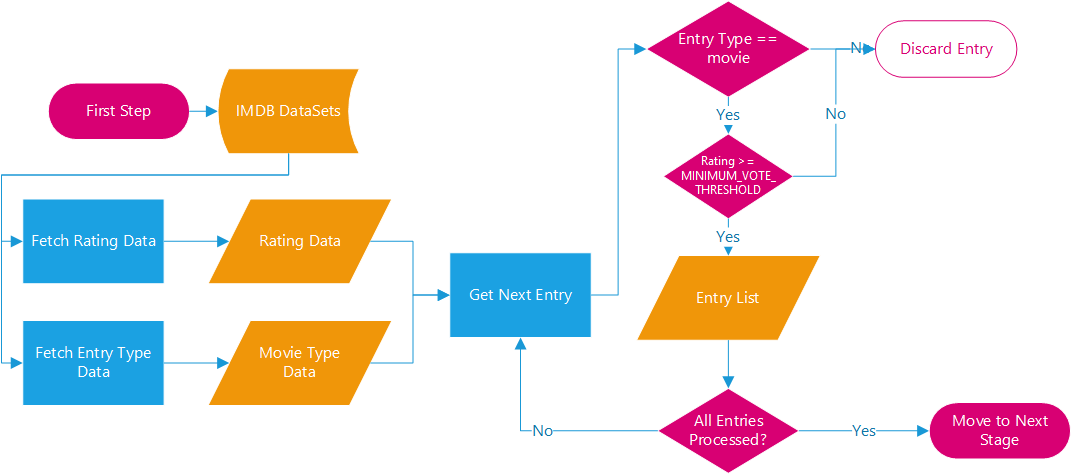
\includegraphics[width=150mm]{Chapters/5 - Architecture/Import/Images/imdb_flowchart.png}
  \caption{Διάγραμμα ροής δεδομένων από IMDB}
  \label{flowchart:imdbImport}
\end{figure}
\subsection{Βήμα 2ο - Δεδομένα από TMDb}
Στο 2ο βήμα αφού έχουμε τα δεδομένα που χρειάζονται από το πρώτο, δημιουργεί και προγραμματίζει για εκτέλεση ασύγχρονα ερωτήματα ζητώντας πλήρη δεδομένα ταινιών για κάθε αναγνωριστικό ταινίας που έχουμε στην υπηρεσία TMDb. 

Ο στόχος δεν είναι μόνο η απόκτηση δεδομένων ταινιών αλλά και συντελεστών, εταιριών και χωρών παραγωγής, και ειδών ταινιών, συνεπώς αφού πάρει τα δεδομένα ταινιών θα χρονοδρομολογήσει και άλλα ασύγχρονα ερωτήματα στην εν λόγω υπηρεσία για να πάρει και τα υπόλοιπα δεδομένα. 

Αφού τελειώσει αυτή η διαδικασία, συσχετίζει όλα τα δεδομένα μεταξύ τους και τα εισάγει στην βάση δεδομένων για περαιτέρω επεξεργασία από κάποιο άλλο σύστημα. 
\begin{figure}[h]
  \centering
  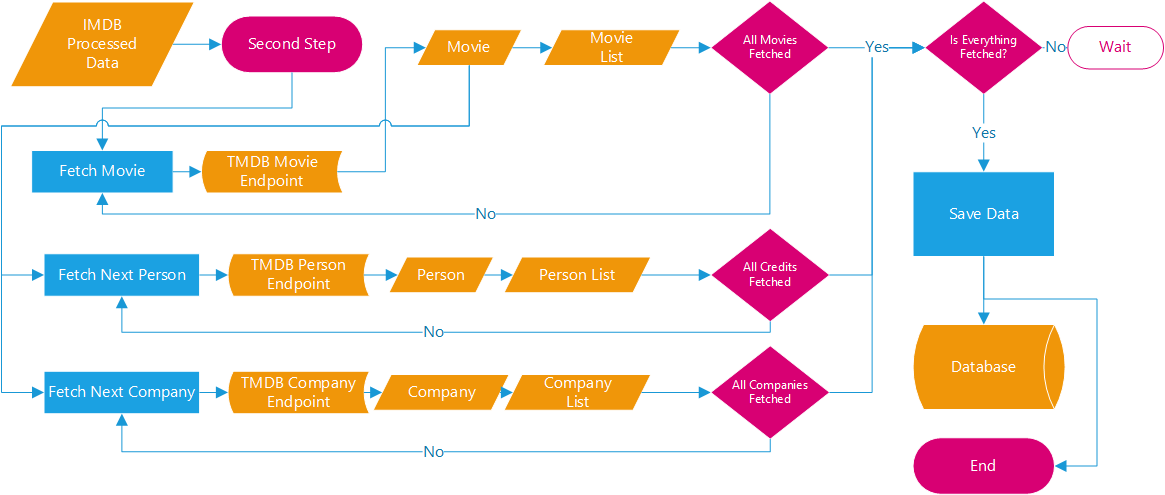
\includegraphics[width=150mm]{Chapters/5 - Architecture/Import/Images/tmdb_flowchart.png}
  \caption{Διάγραμμα ροής δεδομένων από TMDb}
  \label{flowchart:tmdbImport}
\end{figure}
\section{Σύστημα επεξεργασίας δεδομένων}
Ο Ρόλος του Συστήματος επεξεργασίας δεδομένων είναι να πάρει τα ανεπεξέργαστα δεδομένα από την βάση δεδομένων και να δημιουργήσει σχέσεις μεταξύ τους κατηγοριοποιώντας τα. Η Εφαρμογή προσφέρει δεδομένα ανά 4 κατηγορίες, και παράλληλα για κάθε κατηγορία ανά χρονολογική περίοδο. Η κατηγοριοποίηση είναι βασισμένη στα παρακάτω στοιχεία:
\begin{itemize}
    \item Στοιχεία ανά χώρα παραγωγής
    \item Στοιχεία ανά εταιρία παραγωγής
    \item Στοιχεία ανά συντελεστή - ξεχωριστά ανά ηθοποιό, συγγραφέα, σκηνοθέτη και παραγωγό
    \item Στοιχεία ανά είδος ταινίας
\end{itemize}

Η κάθε κατηγορία περιέχει στοιχεία για
την ταινία με την μεγαλύτερή αξιολόγηση, 
την ταινία με την χαμηλότερη αξιολόγηση, 
την μέση βαθμολογία ταινιών για αυτήν την κατηγορία, 
τις ταινίες με τα μεγαλύτερα και τα μικρότερα έσοδα και έξοδα, 
τα μέσα έξοδα / έσοδα ταινιών, 
τον πιο δημοφιλή και λιγότερο δημοφιλή ηθοποιό (ή συμπρωταγωνιστή αν η κατηγορία είναι ανά συντελεστή -- ηθοποιό), 
παραγωγό (η συμπαραγωγό αν η κατηγορία είναι ανά συντελεστή -- παραγωγό), 
σκηνοθέτη (η συν-σκηνοθέτη αν η κατηγορία είναι ανά συντελεστή -- σκηνοθέτη) και 
συγγραφέα (ή συν-συγγραφέα αν η κατηγορία είναι ανά συντελεστή -- συγγραφέα), 
την πιο δημοφιλή και λιγότερο δημοφιλή χώρα παραγωγής (η συμπαραγωγής αν η κατηγορία είναι ανά χώρα παραγωγής), 
την πιο δημοφιλή και λιγότερο δημοφιλή εταιρία παραγωγής (ή συμπαραγωγής αν η κατηγορία είναι ανά εταιρία παραγωγής) κ.α
όπως φαίνονται στο σχήμα ~\ref{model:movieinsights}.

\begin{figure}[p]
    \vspace*{-1cm}
    \hspace*{-1cm}
    \makebox[\linewidth]{
        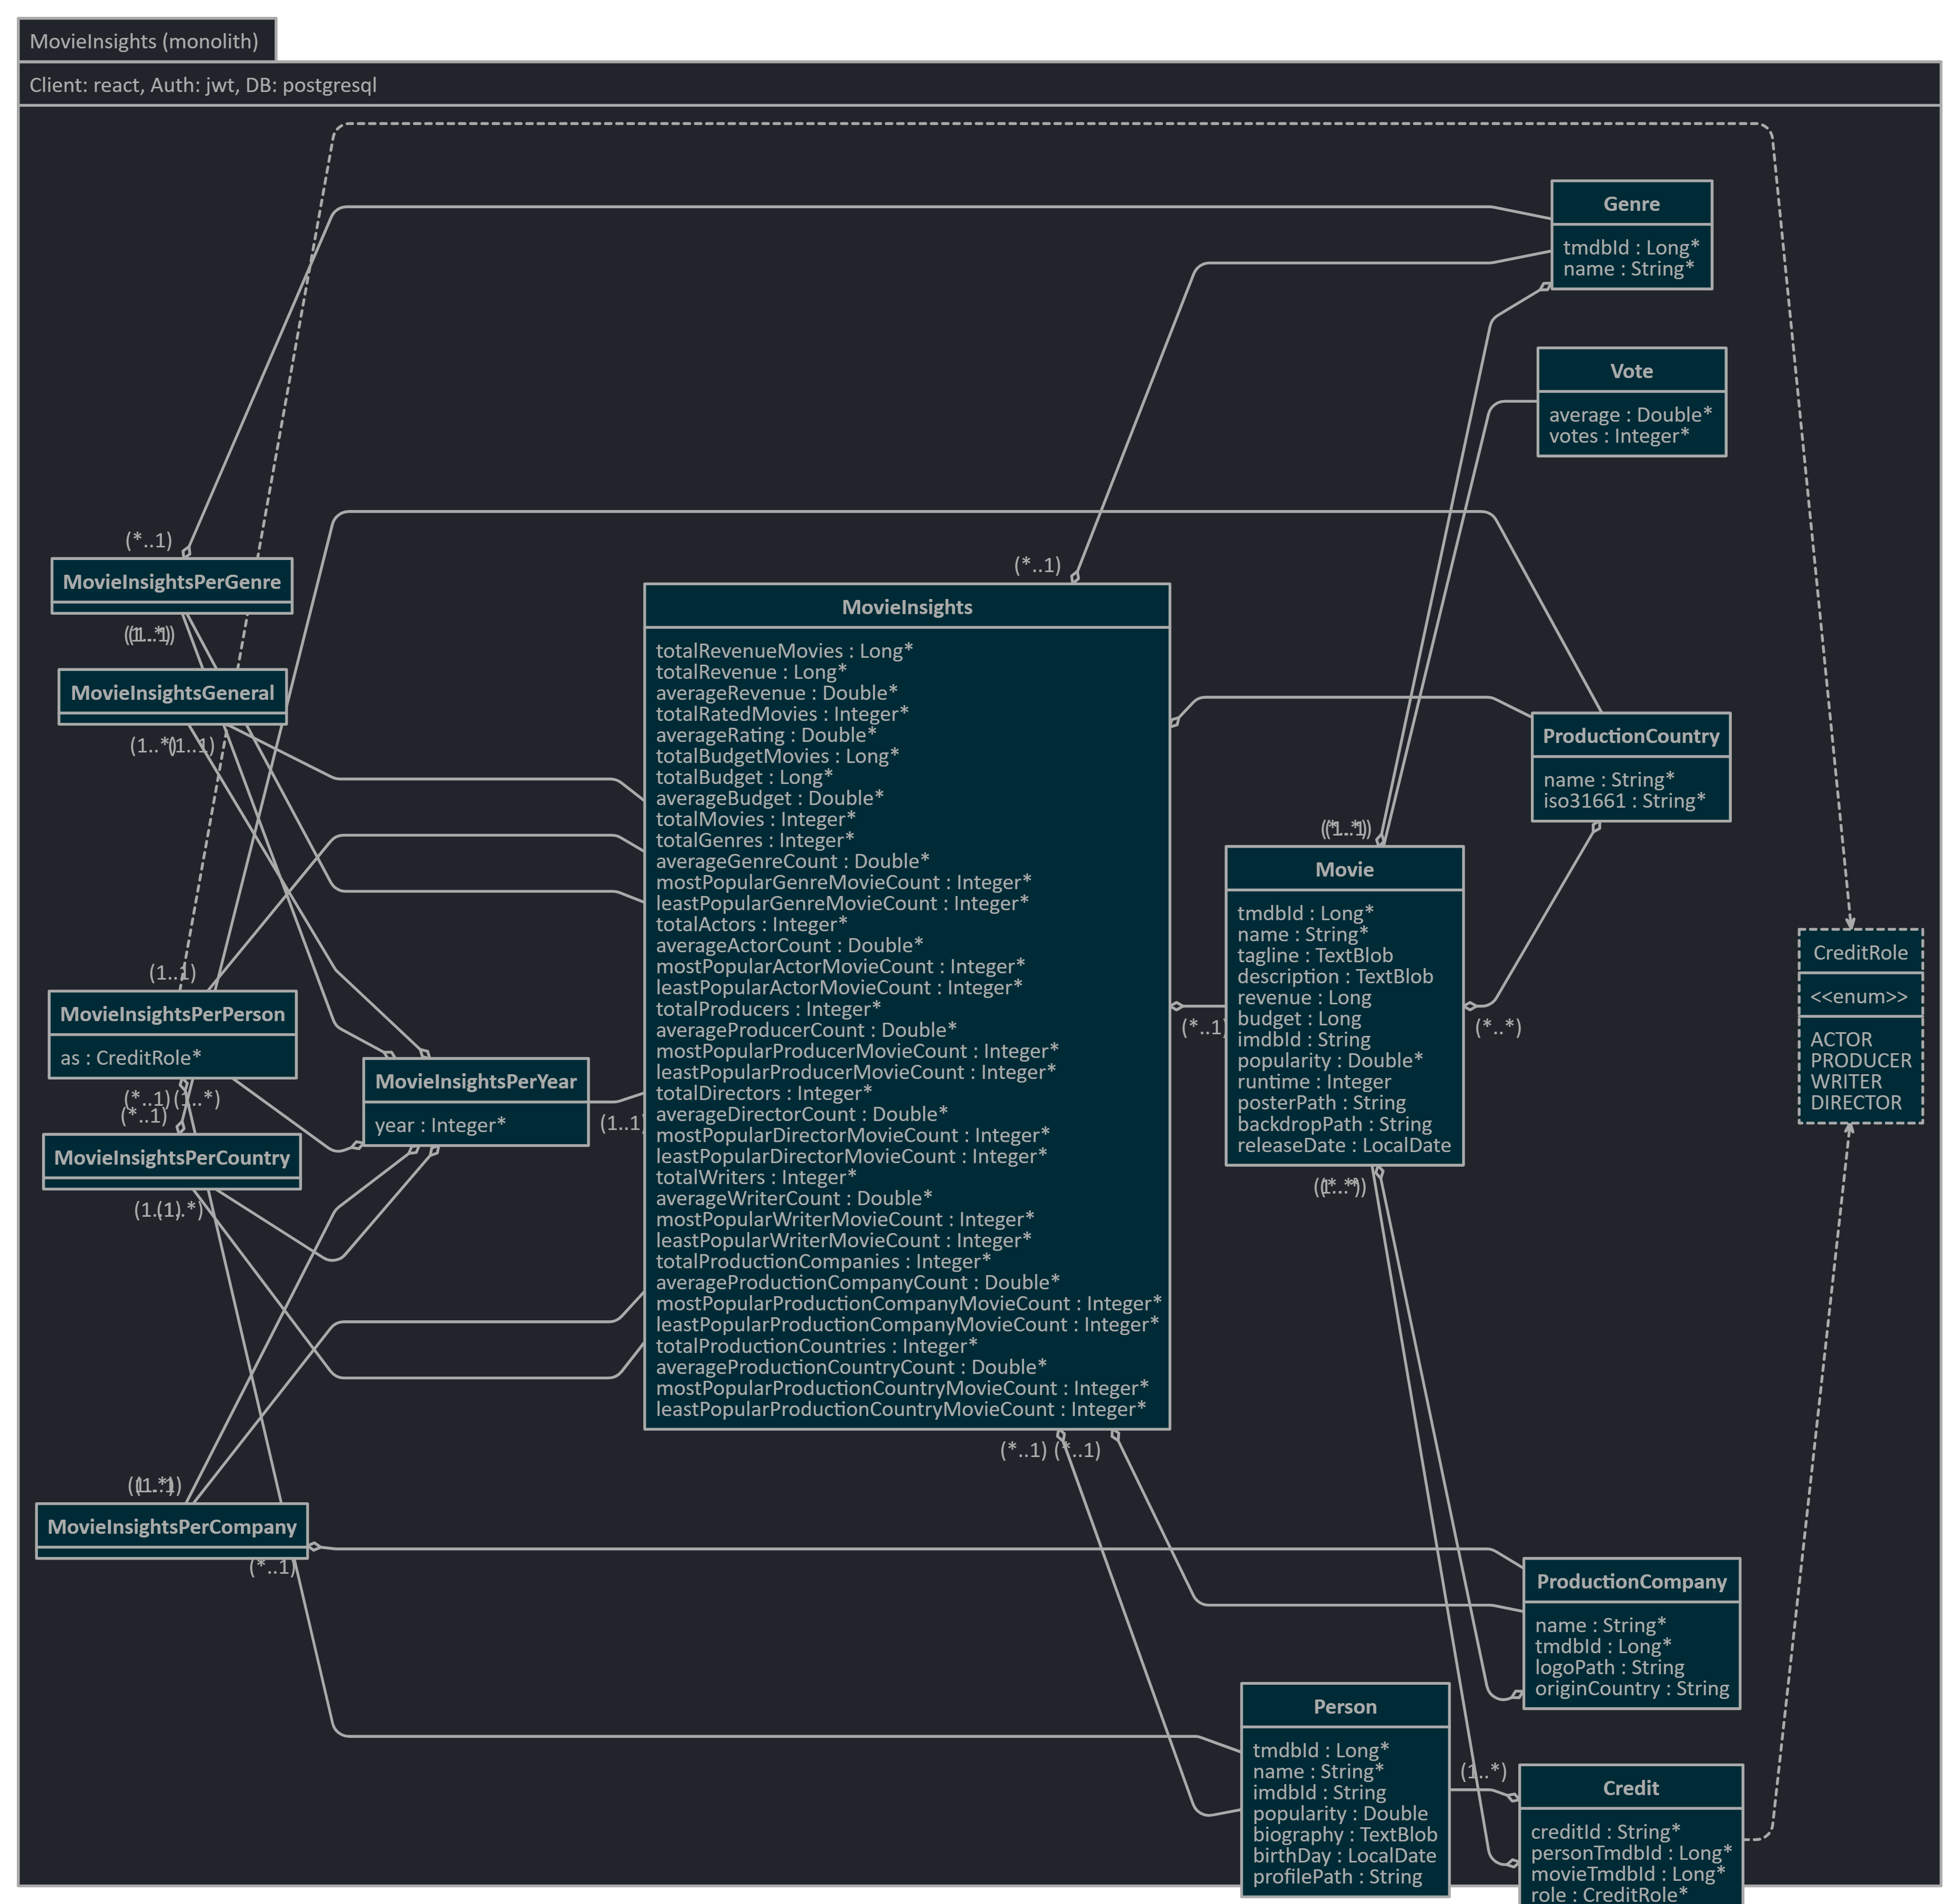
\includegraphics[width=1.4\linewidth]{Chapters/5 - Architecture/MovieInsights/Images/jhipster-jdl (2).png}
    }
   \caption{Μοντελο MovieInsights}
   \label{model:movieinsights}
\end{figure}

Η επεξεργασία των δεδομένων μπορούσε να γίνει είτε στο κομμάτι της βάσης δεδομένων με SQL είτε στο κομμάτι του Server με την Java. Ο πιο αποδοτικός τρόπος είναι να γίνει στην βάση δεδομένων με την SQL καθώς υπάρχουν διάφορα συστήματα βελτιστοποίησης τα οποία επιτρέπουν την επεξεργασία των δεδομένων αποδοτικά και γρήγορα, αλλά σε αυτήν την πτυχιακή προτιμήθηκε η Java για λόγους απλότητας.

Το σύστημα επεξεργασίας χωρίζεται σε 3 διαφορετικά κομμάτια. Το πρώτο κομμάτι συλλέγει και κατηγοριοποιεί τα δεδομένα. Το δεύτερο κομμάτι υπολογίζει τα μέγιστα τα ελάχιστα και τους μέσους των δεδομένων. Το τρίτο
κομμάτι μετατρέπει τα δεδομένα σε μια φιλική προς τη βάση δεδομένων μορφή και τα αποθηκεύει.

\subsection{Βήμα 1 - Κατηγοριοποίηση δεδομένων}
\begin{figure}[H]
    \begin{javacode}
    categories = new HashMap<>();
    getMovieInsights(long id, BaseWrapper<?> o) {
        if (categories.containsKey(id)) {
            return categoriess.get(id);
        }
        IMovieInsightsWrapper wrapper = createMovieInsightsWrapper(o);
        categories.put(id,wrapper);
        return wrapper;
    }
    getMovieInsightObjectsOptimized(Movie movie) {
     // return set of getMovieInsights(...)
    }
    categorizeData(Movie movie) {
        Set<IMovieInsightsWrapper> miSet = getMovieInsightObjectsOptimized(movie);
        miSet.forEach(wrapper -> {
            wrapper.submitMovie(movie);
        });
    }
    Lists
      .partition(dto.movies, 1000)
      .forEach(chunk -> {
         chunk.forEach(this::categorizeData);
      });
    \end{javacode}
    \caption{Σειριακή κατηγοριοποίηση με HashMap}
   \label{code:categorieSerialWithHM}
\end{figure}
Ο Αλγόριθμός κατηγοριοποίησης συλλέγει τα δεδομένα, τα προσθέτει στις ανάλογες κατηγορίες, δημιουργεί τις κατηγορίες αν δεν υπάρχουν, και ετοιμάζει τα δεδομένα για τον τελικό υπολογισμό.

Υπήρξαν πολλές αναθεωρήσεις του αλγορίθμου μέχρι την τελική του έκδοση. Οι περισσότερες αφορούσαν βελτιστοποιήσεις απόδοσης. 

Ο Αρχικός κώδικας (βλ σχήμα: \ref{code:categorieSerialWithHM}) ήταν αρκετά απλός. Είχε HashMaps για την αποθήκευση των δεδομένων ανά κατηγορία, και γινόταν συνεχώς έλεγχοι για το αν υπήρχαν τα δεδομένα. Αν όχι τα δημιουργούσε αλλιώς τα μορφοποιούσε.

Αρχικά ο κώδικας έτρεχε σειριακά, καθώς όμως αυξανόταν τα δεδομένα, ανέβαινε εκθετικά και ο χρόνος κατηγοριοποίησης τους. Για παράδειγμα για 1000 ταινίες μαζί με τους συντελεστές, τις εταιρίες και χώρες παραγωγής και τα είδη των ταινιών τους, έκανε 25 λεπτά για την ολοκλήρωση της κατηγοριοποίησης. Για 5000 ταινίες έκανε πάνω από 8 ώρες. 

Ο κώδικας ξαναγράφτηκε (βλ σχήμα: \ref{code:categorieParallelWithCHM}) για να τρέχει με παραλληλισμό. Έτσι κάποια βασικά στοιχεία άλλαξαν, όπως τα HashMaps έγιναν ConcurrentHashMaps και κάποια άλλα κομμάτια έγιναν Synchronize για να υπάρχει Thread Safety. Το αποτέλεσμα αυτών των αλλαγών ήταν η κατηγοριοποίηση 8000 ταινιών, συνυπολογίζοντας και τα λοιπά σχετικά στοιχεία, να ολοκληρώνεται εντός 25 λεπτών.

\begin{figure}[h]
    \begin{javacode}
    categories = new ConcurrentHashMap<>();
    categorizeData(Movie movie) { // ...
        miSet.parallelStream().forEach // ...
    }
    Lists
      // ...
         chunk
            .parallelStream().forEach // ...
      
    \end{javacode}
    \caption{Παράλληλης κατηγοριοποίηση με ConcurrentHashMap}
   \label{code:categorieParallelWithCHM}
\end{figure}

Στην πορεία εμφανίστηκε ένα πρόβλημα απόδοσης, το οποίο δεν ήταν ορατό κατά την πρώτη υλοποίηση, και το οποίο αφορούσε τα HashMaps.
Ενώ δίνουν με μεγάλη ευκολία, είναι στην ουσία ένα Indexer για την αποθήκευση key-value pairs, έχουν μεγάλο performance-pentalty όταν αρχίζει και μεγαλώνει ο όγκος των ανατεθειμένων δεδομένων και το πρόβλημα μεγεθύνεται ακόμα πιο πολύ όταν είναι και ConcurrentHashMaps λόγω των ελέγχων που γίνονται για το Thread Safety. Ένα δείγμα 30000 ταινιών έκανε πάνω από 4.5 ώρες για να κατηγοριοποιήθει.

Κάτι έπρεπε να αντικαταστήσει τα HashMaps. Στην τελική έκδοση του αλγόριθμου (βλ σχήμα: \ref{code:categorieParallelWithArr}) τα HashMaps αντικαταστάθηκαν με τα Native Arrays. Η επιλογή αυτή είχε ιδιαιτέρως θετικό αντίκτυπο στην ταχύτητα της κατηγοριοποίησης αλλά μεγάλωσε η πολυπλοκότητα διαχείρισης των δεδομένων.
Συγκριτικά με τη χρήση ConcurrentHashMaps, όπου η κατηγοριοποίηση 30.000 ταινιών εκτελούνταν σε 4,5 ώρες, ο ανανεωμένος αλγόριθμος κατηγοριοποίησε 30000 ταινίες σε μόλις 8 λεπτά. 

\begin{figure}[h]
    \begin{javacode}
    creditsArray = new MovieInsightsPersonWrapper[dto.maxPersonId][CreditRole.getSize()];
    companiesArray = new MovieInsightsCompanyWrapper[dto.maxCompanyId];
    countriesArray = new MovieInsightsCountryWrapper[dto.maxCountryId];
    genresArray = new MovieInsightsGenreWrapper[dto.maxGenreId];
    
    getMovieInsights(long id, BaseWrapper<?> o, IMovieInsightsWrapper[] array) {
        synchronized (array) {
            IMovieInsightsWrapper wrapper;
            if ((wrapper = array[(int) id]) == null) {
                array[(int) id] = wrapper = createMovieInsightsWrapper(o);
            }
            return wrapper;
        }
    }
    \end{javacode}
    \caption{Παράλληλη κατηγοριοποίηση με Arrays}
   \label{code:categorieParallelWithArr}
\end{figure}
Ο αλγόριθμος λοιπόν κατηγοριοποιεί τα δεδομένα όπως φαίνεται στο σχήμα \ref{flowchart:categorizeData} και αφού τελειώσει προχωράει στο βήμα 2 του υπολογισμού των δεδομένων.
\begin{figure}[H]
  \centering
  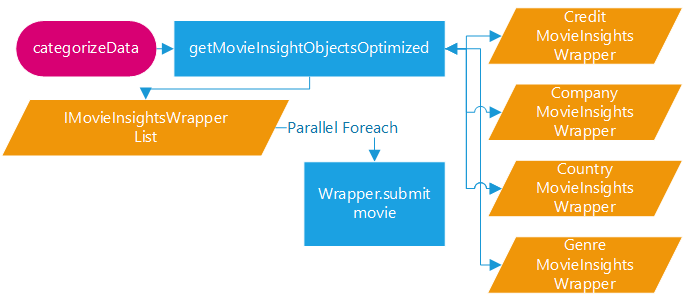
\includegraphics[width=150mm]{Chapters/5 - Architecture/MovieInsights/Images/categorizeData.png}
  \caption{Διάγραμμα ροής κατηγοριοποίησης δεδομένων}
  \label{flowchart:categorizeData}
\end{figure}
\subsection{Βήμα 2 - Υπολογισμός  δεδομένων}

Επιλέγοντας την γλώσσα προγραμματισμού Java για τον υπολογισμό των δεδομένων και επικεντρώνοντας όλες τις βελτιστοποιήσεις στο κομμάτι τις απόδοσης, δημιουργήθηκε ένα νέο πρόβλημα. Επειδή υπάρχουν διπλότυπα δεδομένα λόγω της φύσης της δομής της πτυχιακής, η παρούσα υλοποίηση δεν είναι καθόλου βελτιστοποιημένη για την χρήση μνήμης RAM. Στο πέρας του πρώτο βήματος με δεδομένα 30000 ταινιών κατηγοριοποιημένα, η χρήση μνήμης ξεπερνάει τα 25 GB. Έχοντάς αυτό σαν δεδομένο ο αλγόριθμος υπολογισμού των δεδομένων εκτός από αποδοτικός ως προς την ταχύτητα θα έπρεπε να είναι τουλάχιστον και αποδοτικός ως προς την χρήση μνήμης.

Η αρχική προσέγγιση ήταν ο υπολογισμός των δεδομένων σε κάποια DTO με σκοπό ύστερα την δημιουργία Managed Entities του Hibernate, για να μπορέσουν να αποθηκευτούν στην βάση δεδομένων. Με αυτόν τον τρόπο όμως θα είχαμε ξανά το φαινόμενο των διπλότυπων και θα ξοδεύαμε ακόμα περισσότερη μνήμη καθώς η πλειοψηφία των δεδομένων είναι Native Ints, Longs και Doubles και όχι τόσο Reference Types. Η προσέγγιση που επιλέχτηκε ήταν η δημιουργία ενός Wrapper που κληρονομεί από το Maanaged Entity του Hibernate, κάνοντας και το Wrapper, Managed Entity. Με λίγες ρυθμίσεις πλέον το Wrapper μπορεί να σταλεί απευθείας στον Hibernate για να αποθηκευτεί στην βάση δεδομένων χωρίς να χρειαστεί η δημιουργία κάποιου άλλου Managed Entity.

Για αυτόν τον λόγο ο αλγόριθμος της επεξεργασίας δεδομένων μεταφέρθηκε μέσα σε αυτό το Wrapper έτσι ώστε να μπορεί να τρέξει μετά το πέρας της κατηγοριοποίησης αποδοτικά. Βλέποντας πίσω στο σχήμα(\ref{code:categorieParallelWithCHM}) είναι εμφανές ότι αποστέλλεται μια ταινία στον Wrapper για περαιτέρω επεξεργασία. 

Για να βελτιστοποιηθεί ακόμα περισσότερο στο βήμα της κατηγοριοποίησης ο Wrapper εκτελεί όσους υπολογισμούς μπορεί, που δεν χρειάζονται τα συνολικά δεδομένα για να υπολογιστούν, αλλά μόνο τα υπάρχοντα κάθε φορά σε κάθε submit.

Τα δεδομένα που υπολογίζονται σε κάθε submit είναι οι ταινίες με την μεγαλύτερη και χαμηλότερη βαθμολογία καθώς και η μέση βαθμολογία ταινιών για κάθε κατηγορία και οι ταινίες με τα μεγαλύτερα και χαμηλότερα έσοδα/έξοδα καθώς και τα μέσα έσοδα/έξοδα για κάθε κατηγορία. Τα υπόλοιπα δεδομένα υποβάλλονται και αποθηκεύονται σε HashMaps για τον τελικό υπολογισμό.

Ένα πρόβλημα που αντιμετωπίστηκε στον υπολογισμό της ταινίας με την μεγαλύτερη βαθμολογία ήταν η ακρίβεια της βαθμολογίας. Για παράδειγμα δεν είναι το ίδιο να υπάρχει μια ταινία με βαθμολογία 9.0 και 10.000 ψήφους και μια άλλη ταινία με βαθμολογία 9.0 και 200.000 βαθμολογίες. Όπως επίσης είναι πιο αξιόπιστη μια βαθμολογία για παράδειγμα 8.5 με 2.000.000 ψήφους από ότι μια βαθμολογία 9.0 με 100.000 ψήφους. 

Για την επίλυση αυτού του προβλήματος χρησιμοποιήθηκε ένας πολύ απλός αλγόριθμος βάρους $rating * \log_2(voteCount)$, έτσι ώστε να υπολογίζονται και οι ψήφοι και να βγαίνει ενα "σκορ" ταινίας το οποιο θα συγκρίνεται με τα άλλα "σκορ" ταινιών έτσι ώστε να υπολογίζεται η με μεγαλύτερη ακρίβεια ποια ταινία είχε την μεγαλύτερη βαθμολογία.
\begin{figure}[h]
    \begin{javacode}
double calculateScore(Vote vote, boolean high) {
    return getScore(vote.getAverage(), vote.getVotes(), high, 2);
}
double getScore(double value, double weight, boolean high, int base) {
    double weightLog = Math.log(weight) / Math.log(base);
    return high ? value * weightLog : value / weightLog;
}
    \end{javacode}
    \caption{Αλγόριθμος Βάρους Βαθμολογιών}
   \label{code:logarithmicScore}
\end{figure}

Με τον παραπάνω αλγόριθμο σαν βάση, ο Αλγόριθμος υπολογισμού των ταινιών με την μεγαλύτερη και χαμηλότερη βαθμολογία καθώς και της μέσης βαθμολογίας έχει διαμορφωθεί όπως φαίνεται στο σχήμα ~\ref{code:ratingCalculation}. Αρχικά γίνεται έλεγχος αν οι ψήφοι της βαθμολογίας της εν λόγω ταινίας είναι περισσότεροι ή ίσοι με την τιμή της σταθεράς {\it MINIMUM\_VOTES\_THRESHOLD}. Αν δεν είναι, η ταινία εξαιρείται από αυτόν τον υπολογισμό. Αλλιώς προστίθεται η βαθμολογία της ταινίας σε μια μεταβλητή που κρατάει το άθροισμά όλων των βαθμολογιών και αυξάνεται η μεταβλητή που κρατάει και πόσες ταινίες έχουν υποβάλει τις βαθμολογίες τους, για να υπολογιστεί αργότερα η μέση βαθμολογία ταινιών. Ύστερα αν δεν υπάρχει ήδη ταινία με την μεγαλύτερη η χαμηλότερη βαθμολογία τοποθετείται αυτή για την οποία γίνεται ο έλεγχος αυτήν την χρονική στιγμή, αλλιώς γίνεται έλεγχος αν αυτή η ταινία έχει μεγαλύτερη / μικρότερη βαθμολογία από την ανάλογη υπάρχουσα και ορίζεται αυτή στην θέση της σε περίπτωση που πληροί της προϋποθέσεις.

\begin{figure}[h]
    \begin{javacode}
void submitRating(Movie movie) {
    if (movie.getVote().getVotes() >= Constants.MINIMUM_VOTES_THRESHOLD) {
        synchronized (voteLock) {
            Vote vote = movie.getVote();
            totalVoteAverage += vote.getAverage();
            setTotalRatedMovies(getTotalRatedMovies() + 1);
            if (getHighestRatedMovie() == null) {
                setHighestRatedMovie(movie);
            } else {
                setHighestRatedMovie(calculateVote(calculateScore(getHighestRatedMovie().getVote(), true), getHighestRatedMovie(),calculateScore(movie.getVote(), true),movie,(current, challenger) -> current < challenger));
            }
            if (getLowestRatedMovie() == null) {
                setLowestRatedMovie(movie);
            } else {
                setLowestRatedMovie(calculateVote( getLowestRatedMovie().getVote().getAverage(),getLowestRatedMovie(), movie.getVote().getAverage(),movie,(current, challenger) -> current > challenger));
            }
        }
    }
}   
    \end{javacode}
    \caption{Αλγόριθμος Υπολογισμού Βαθμολογιών}
   \label{code:ratingCalculation}
\end{figure}

Ο υπολογισμοί των ταινιών με τα μεγαλύτερα, μικρότερα και μέσα έσοδα / έξοδα γίνεται με έναν πολύ παρόμοιο τρόπο όπως των βαθμολογιών των ταινιών, χωρίς βέβαια να χρησιμοποιείται ο αλγόριθμος βάρους.

Ο υπολογισμός των υπόλοιπων δεδομένων γίνεται μετά το πέρας του βήματος της κατηγοριοποίησης. Για να γίνει πιο εύκολος ο υπολογισμός, αντί να υποβάλλονται τα δεδομένα ως έχουν έχουν δημιουργηθεί Wrappers γύρο από αυτά για την προσθήκη επιπρόσθετων δεδομένων και λειτουργιών που καθιστούν τον υπολογισμό των δεδομένων πιο εύκολο. Για παράδειγμα ένα αντικείμενο τύπου Genre έχει το ανάλογο GenreWrapper, όπως επίσης και ένα αντικείμενο τύπου Person έχει ανάλογα ActorWrapper, DirectorWrapper, ProducerWrapper και WritterWrapper για κάθε κατηγορία ατόμου που υποστηρίζεται από την εφαρμογή. Σε αυτά τα Wrappers υπάρχουν δεδομένα όπως ο αριθμός ταινιών που συμμετέχουν αυτά τα Wrappers για αυτήν την κατηγορία, οι ταινίες οι ίδιες, και υπάρχουν και λειτουργίες σύγκρισης (Comparators) μεταξύ ίδιων Wrappers χρησιμοποιώντας αυτά τα παραπάνω δεδομένα.

Όταν γίνεται η υποβολή δημιουργείται αρχικά ένα Wrapper προσθέτοντάς μεταδεδομένα χωρίς να ελεγχθεί αν υπάρχει ήδη Wrapper που να αναφέρεται στο ίδιο αντικείμενο, αποθηκευμένο στο ανάλογο HashMap οπως φαίνεται στο σχήμα \ref{code:submitGenre}, στην σειρά 5 για την υποβολή δεδομένων ειδών ταινιών.
\begin{figure}[h]
    \begin{javacode}
void submitGenres(Movie movie) {
    AtomicBoolean hasIncreased = new AtomicBoolean(false);
    movie.getGenres().parallelStream().filter(Objects::nonNull).forEach(genre -> {
        calculateTotals(genreTotals, hasIncreased);
        submit(new GenreWrapper(genre, processor.getMovieCount(genre)), genres, movie, genre);
    });
}
    \end{javacode}
    \caption{Αλγόριθμος Υποβολής Δεδομένων Είδους Ταινίας}
    \label{code:submitGenre}
\end{figure}

Στην γενικευμένη συνάρτηση submit πάραυτα γίνεται εκεί ο έλεγχος για την ύπαρξη του ανάλογου Wrapper, και αν υπάρχει απλά αγνοεί το νέο Wrapper και αλλάζει το υπάρχων χρησιμοποιώντας τα στοιχεία του νεου, αλλιώς τοποθετεί το δημιουργημένο Wrapper στο ανάλογο HashMap όπως φαίνεται στο σχήμα \ref{code:submit}.

\begin{figure}[h]
    \begin{javacode}
<T extends IdentifiedEntity, W extends BaseWrapper<T>> void submit(W wrapper, Map<Long, W> objMap, Movie movie, T obj) {
    W wrapper2;
    synchronized (objMap) {
        if ((wrapper2 = objMap.putIfAbsent(obj.getId(), wrapper)) == null) {
            wrapper2 = wrapper;
        }
    }
    wrapper2.movies.add(movie);
    wrapper2.count++;
}
    \end{javacode}
    \caption{Αλγόριθμος Γενικευμένης υποβολής δεδομένων}
    \label{code:submit}
\end{figure}

Επιπρόσθετα για τον υπολογισμό αυτών των δεδομένων χρησιμοποιείται μια βοηθητική γενικευμένη κλάση Total, η οποία κρατάει τα στοιχεία για τα μέγιστα, ελάχιστα και μέσα αυτών των δεδομένων. 

Μετά το πέρας της συλλογής και της κατηγοριοποίησης των δεδομένων, το κάθε MovieInsights Wrapper ξεχωριστά θα υπολογίσει τα υπόλοιπα δεδομένα για το ίδιο αλλά και για κάθε εξαρτώμενο Wrapper από αυτό, που στην συγκεκριμένη περίπτωση τα εξαρτώμενα Wrappers, είναι οι κατηγορίες ανά χρόνο.

Για κάθε διαφορετικό Wrapper HashMap θα υπολογιστούν τα μέγιστα και τα ελάχιστα χρησιμοποιώντας τις συναρτήσεις σύγκρισης που υπάρχουν μέσα στα Wrappers, και τα δεδομένα που περιέχουν τα μέγιστα και τα ελάχιστα θα υποβληθούν στα αντικείμενα της βοηθητικής κλάσης Total για την ανάκτηση τους αργότερα, όπως φαίνεται στα σχήματα \ref{code:calculateChildInsights} και \ref{code:getWrapperBasedOnComparator}.

\begin{figure}[h]
    \begin{javacode}
<W extends BaseWrapper<WE>, WE> void calculateChildInsights(Map<Long, W> map, Comparator<? super W> comparator, Total<WE> totals) {
    Optional<W> mostPopularEntryResult = getWrapperBasedOnComparator(map, comparator.reversed());
    mostPopularEntryResult.ifPresent(totals::submitMostPopular);
    Optional<W> leastPopularEntryResult = getWrapperBasedOnComparator(map, comparator);
    leastPopularEntryResult.ifPresent(totals::submitLeastPopular);
    totals.setTotalEntities(map.size());
}
    \end{javacode}
    \caption{Γενικευμένος Αλγόριθμος υπολογισμού μέγιστων και ελάχιστων δεδομένων}
    \label{code:calculateChildInsights}
\end{figure}
\begin{figure}[h]
    \begin{javacode}
private <W extends BaseWrapper<EW>, EW> Optional<W> getWrapperBasedOnComparator(Map<Long, W> wrapperMap, Comparator<? super W> comparator) {
    return wrapperMap.values().parallelStream().sorted(comparator).filter(e -> (slave ? master.getCategory() : getCategory()) != e.category || e.object != (slave ? master.getSource().object : source.object)).findFirst();
}
    \end{javacode}
    \caption{Γενικευμένος Αλγόριθμος ανάκτησης Wrapper απο ενα HashMap με βάση αλγόριθμο σύγκρισης}
    \label{code:getWrapperBasedOnComparator}
\end{figure}

Τέλος όλα τα δεδομένα αποθηκεύονται στα πεδία της κληρονομουμένης κλάσης MovieInsights, ανακτώντας τα δεδομένα από τα αντικείμενα της βοηθητικής κλάσης Total.

% \begin{figure}[h]
%     \begin{javacode}
% void submitRevenue(Movie movie) {
%     if (movie.getRevenue() >= Constants.MINIMUM_REVENUE_THRESHOLD) {
%         synchronized (revenueLock) {
%             setTotalRevenue(getTotalRevenue() + movie.getRevenue());
%             setTotalRevenueMovies(getTotalRevenueMovies() + 1);
%             if (getHighestRevenueMovie() == null) {
%                 setHighestRevenueMovie(movie);
%             } else {
%                 if (getHighestRevenueMovie().getRevenue() < movie.getRevenue()) {
%                     setHighestRevenueMovie(movie);
%                 } else if (getHighestRevenueMovie().getRevenue().equals(movie.getRevenue()) && movie.getPopularity() > getHighestRevenueMovie().getPopularity()) {
%                     setHighestRevenueMovie(movie);
%                 }
%             }
%             if (getLowestRevenueMovie() == null) {
%                 setLowestRevenueMovie(movie);
%             } else {
%                 if (getLowestRevenueMovie().getRevenue() > movie.getRevenue()) {
%                     setLowestRevenueMovie(movie);
%                 } else if (getLowestRevenueMovie().getRevenue().equals(movie.getRevenue()) && movie.getPopularity() > getLowestRevenueMovie().getPopularity()) {
%                     setLowestRevenueMovie(movie);
%                 }
%             }
%         }
%     }
% }    
%     \end{javacode}
%     \caption{Αλγόριθμος Υπολογισμού Εσόδων}
%   \label{code:revenueCalculation}
% \end{figure}
% \begin{figure}[h]
%     \begin{javacode}
% void submitBudget(Movie movie) {
%     if (movie.getBudget() >= Constants.MINIMUM_BUDGET_THRESHOLD) {
%         synchronized (budgetLock) {
%             setTotalBudget(getTotalBudget() + movie.getBudget());
%             setTotalBudgetMovies(getTotalBudgetMovies() + 1);
%             if (getHighestBudgetMovie() == null) {
%                 setHighestBudgetMovie(movie);
%             } else {
%                 if (getHighestBudgetMovie().getBudget() < movie.getBudget()) {
%                     setHighestBudgetMovie(movie);
%                 } else if (getHighestBudgetMovie().getBudget().equals(movie.getBudget()) && movie.getPopularity() > getHighestBudgetMovie().getPopularity()) {
%                     setHighestBudgetMovie(movie);
%                 }
%             }
%             if (getLowestBudgetMovie() == null) {
%                 setLowestBudgetMovie(movie);
%             } else {
%                 if (getLowestBudgetMovie().getBudget() > movie.getBudget()) {
%                     setLowestBudgetMovie(movie);
%                 } else if (getLowestBudgetMovie().getBudget().equals(movie.getBudget()) && movie.getPopularity() > getLowestBudgetMovie().getPopularity()) {
%                     setLowestBudgetMovie(movie);
%                 }
%             }
%         }
%     }
% }
%     \end{javacode}
%     \caption{Αλγόριθμος Υπολογισμού Εξόδων}
%     \label{code:budgetCalculation}
% \end{figure}
% \begin{javacode*}{frame=none,fontsize=\small,linenos=false}
% void calculateChildInsights(Map<Long, W> map, Comparator<? super W> comparator, Total<WE> totals)
% \end{javacode*}

\subsection{Βήμα 3 - Αποθήκευση δεδομένων}
Έχοντάς συλλέξει, κατηγοριοποιήσει και υπολογίσει όλα τα απαραίτητα δεδομένα, τα δεδομένα αυτά με ελάχιστες μετατροπές στέλνονται στον Hibernate για να αποθηκευτούν στην βάση δεδομένων έτσι ώστε να τεθεί η εφαρμογή σε κατάσταση ετοιμότητας. 

Για την αποθήκευση δεδομένων δημιουργείται μια νέα "συναλλαγή". Η συναλλαγή αυτή βεβαιώνει ότι αν κάποιο από τα δεδομένα αυτά δεν μπορούσε για οποιονδήποτε λόγω να αποθηκευτεί στην βάση δεδομένων, να ακυρωθεί όλη αυτή η διαδικασία και να τερματίσει η εφαρμογή με το ανάλογο μήνυμα σφάλματος, έτσι ώστε να μπορεί να επιλυθεί απο κάποιον διαχειριστή. Η αποθήκευση μερικών δεδομένων στην βάση δεδομένων θα είχε καταστροφικές συνέπειες στην λειτουργία της εφαρμογής. 

Μετά το πέρας της αποθήκευσης, γίνεται εκκαθάριση του Cache και ζητείται να γίνει και εκκαθάριση μνήμης από τον Garbage Collector το JVM, ώστε να ελευθερωθεί μνήμη για την καλύτερη λειτουργία της εφαρμογής. Πολλές φορές αυτό δεν είναι δυνατό ανάλογα με το JVM που χρησιμοποιείται και έτσι μετά την αρχικοποίηση στην περίπτωση που δεν υπάρχει διαθέσιμη μνήμη συστήνεται η επανεκκίνηση της εφαρμογής.


\section{Μηχανή Αναζήτησης}
Η μηχανή αναζήτησης είναι μια σημαντική υπηρεσία για την εφαρμογή και επιτρέπει στον χρήστη την αναζήτηση και αυτόματη συμπλήρωση της αναζήτησης ατόμων, εταιριών παραγωγής, χωρών παραγωγής και ειδών ταινιών. 

Η μηχανή αναζήτησης έχει την δυνατότητα να συνδεθεί σε μια εξωτερική βαση δεδομένων για την ανάκτηση δεδομένων είτε να χρησιμοποιήσει την εσωτερική της βάση δεδομένων. Για την βελτιστοποίηση της εμπειρίας του χρήστη η μηχανή αναζήτησης χρησιμοποιεί την δικιά της βάση δεδομένων, καθώς είναι πολύ πιο γρήγορη απο μια συμβατική SQL βάση δεδομένων, με το μειονέκτημα της διπλοτυπίας δεδομένων. 

Για περαιτέρω βελτιστοποίηση δημιουργήθηκαν ξεχωριστά Indices για την μηχανή αναζήτησης και ξεχωριστά Entities για την βάση δεδομένων. Έχοντάς ως κύρια πηγή της αλήθειας τα Entities της βάσης δεδομένων SQL, τα Indicies της μηχανής αναζήτησης έχουν τα λιγότερα δυνατά δεδομένα που χρειάζονται για την αναζήτηση, μειώνοντας σημαντικά τον απαιτούμενο χώρο αποθήκευσης.

Καθώς όμως τα δεδομένα δεν βρίσκονται σε μια μόνο βάση δεδομένων, χρειάζεται ο συγχρονισμός τους καθ όλη την λειτουργία της εφαρμογής. Αυτό γίνεται εύκολα καθώς τα δεδομένα που χρησιμοποιούνται στην αναζήτηση, αλλάζουν μόνο όταν τρέχει το σύστημα εισαγωγής δεδομένων και αυτό γίνεται μόνο στην εκκίνηση της εφαρμογής.

Πάραυτα καθώς η μηχανή αναζήτησης είναι ένα εξωτερικό σύστημα, όχι άμεσα επιβλεπόμενο απο την εφαρμογή, τα δεδομένα της βάσης δεδομένων της, μπορούν να αλλάξουν και να αλλοιωθούν ανά πάσα στιγμή. Για αυτόν τον λόγο έχει δημιουργηθεί μια υπηρεσία που οι αποκλειστικές αρμοδιότητες της είναι να συγχρονίζει τα δεδομένα της κύριας βάσης δεδομένων με την βάση δεδομένων της μηχανής αναζήτησης. Αυτή η υπηρεσία ενεργεί μια φορά στην εκκίνηση ακριβώς πριν τεθεί η εφαρμογή σε κατάσταση ετοιμότητας, και ενεργεί όταν ένας διαχειριστής το ζητήσει. 

Η Μηχανή Αναζήτησης πέρα απο τον συγχρονισμό δεδομένων επιτρέπει τον χρήστη να αναζητήσει κάτι, αλλα παράλληλα επιτρέπει και την αυτόματη συμπλήρωση. Για να λειτουργήσει η Αυτόματη συμπλήρωση όλα τα Indices έπρεπέ να ρυθμιστούν ανάλογα.

\begin{figure}[H]
    \begin{jsoncode}
{"analysis": {
  "filter": {
    "autocomplete_filter": {
      "type": "edge_ngram",
      "min_gram": 1,
      "max_gram": 40
    }
  },
  "analyzer": {
    "autocomplete_search": {
      "type": "custom",
      "tokenizer": "standard",
      "filter": ["lowercase"]
    },
    "autocomplete_index": {
      "type": "custom",
      "tokenizer": "standard",
      "filter": ["lowercase", "autocomplete_filter"]
    }
  }
}}
    \end{jsoncode}
    \caption{Ρυθμίσεις ενός Index της ElasticSearch}
   \label{config:es}
\end{figure}

Για να λειτουργήσει η αυτόματη συμπλήρωση κάθε λέξη και πρόταση μέσα σε αυτά τα Indices έπρεπε να χωριστεί σε ngrams. Όπως φαίνεται στο σχήμα \ref{config:es} στην σειρά 18, δηλώθηκε ενα φίλτρο το οποίο σπάει τις λέξεις και προτάσεις σε ngrams και ετσι επιτρέπει την ρύθμιση ενός πεδίου ενός Index για να μπορεί να αναζητηθεί με αυτόματη συμπλήρωση.

Το επόμενο βήμα ήταν να δηλωθούν τα πεδία στα Indices που θα έχουν τα φίλτρα του autocomplete, όπως φαίνεται στο σχήμα \ref{code:index}

\begin{figure}[h]
    \begin{javacode}
@MultiField(
    mainField = @Field(
        type = Text, 
        fielddata = true,
        analyzer = "autocomplete_index", 
        searchAnalyzer = "autocomplete_search"),
    otherFields = {@InnerField(suffix = "verbatim", type = Keyword)})
private String name;
    \end{javacode}
    \caption{Annotations ενός Index της ElasticSearch}
   \label{code:index}
\end{figure}

Με αυτόν τον τρόπο δηλώνονται τα Indices στον κώδικα με τις σωστές ρυθμίσεις, και η βιβλιοθήκη που χρησιμοποιήθηκε για να επικοινωνήσει με την ElasticSearch, Jest αρχικοποιεί τα Indices στην ElasticSearch και αφου προστεθούν δεδομένα απο τον συγχρονισμό των 2 βάσεων, η μηχανή αναζήτησης είναι έτοιμη για χρήση.

Καθώς όπως προαναφέρθηκε η ElasticSearch είναι ένα αυτόνομο σύστημα πρέπει να του δοθεί ενα ανάλογο Query που να μπορεί να το καταλάβει για να μπορέσει να σερβίρει τα δεδομένα. Αυτό το κάνει η υπηρεσία SearchService.

Όλα τα entities της εφαρμογής έχουν το ανάλογο Service για να επιτρέψουν την ανάκτηση, μορφοποιήση, δημιουργεία αλλα και διαγραφή των δεδομένων τους, γνωστό ως CRUD. Τα Entities που έχουν ανάλογα Indicies μοιράζονται τα ίδια Services για λόγους απλότητας και συγκέντρωσης των αρμοδιοτήτων σε ενα σημείο. 

Κάθε υπηρεσία ενός Entity που έχει παράλληλα και Index, κάνει εγγραφή στο SearchService κατα την εκκίνηση, έτσι ώστε οταν φτάσει η στιγμή που θα γίνει ένα ερώτημα αναζήτησης, το SearchService να γνωρίζει απο ποια Indices θα παρθούν τα δεδομένα. Το κάθε Service που γίνεται register ορίζει επίσης ένα Query. Με αυτόν τον τρόπο η μηχανή αναζήτησης δεν χρειάζεται να γνωρίζει τίποτα για τα Indices, απλά παίρνει τα ερωτήματα απο όλα τα Services που δηλώνουν Indices, τα συνδιάζει και τα στέλνει στην ElasticSearch. Οταν πάρει τα δεδομένα, τα αλλάζει μορφή και τα στέλνει στον Client σε μια διαφορετική μορφή για την βελτιστοποίηση του μεγέθους της απάντησης. 

Όταν γίνεται η αυτόματη συμπλήρωση, για κάθε γράμμα που πληκτρολογείται στον Client, γίνεται και ένα ερώτημα στον Server και στην Μηχανή Αναζήτησης. Είναι πολύ σημαντικό και η μηχανή αναζήτησης να σερβίρει τα δεδομένα πολύ γρήγορα, αλλα και ο Server να απαντάει πολύ γρήγορα. Πέρα απο την ταχύτητα που θα απαντάει ο Server, πρέπει επίσης η απάντηση να είναι μικρή έτσι ώστε πρώτον να εξοικονομεί δεδομένα απο clients οι οποίοι βρίσκονται σε Metered Connections, και να στέλνονται πιο γρήγορα τα αποτελέσματα σε Clients οι οποίοι έχουν χαμηλή ταχύτητα Internet.

Για παράδειγμα το αποτέλεσμα της αναζήτησης που επιστρέφει η μηχανή αναζήτησης όπως φαίνεται στο σχήμα \ref{result:es} έχει μέγεθος 420 bytes για ένα αποτέλεσμα με μέγεθος αποτελέσματος 232 bytes, σε αντίθεση με το αποτέλεσμα του SearchService όπως φαίνεται στο σχήμα \ref{result:ss} με μέγεθος 166 bytes, για ένα αποτέλεσμα με μέγεθος αποτελέσματος 123 bytes. Είναι εμφανές λοιπόν οτι με την βελτιστοποίηση το μέγεθος της απάντησης είναι πολύ μικρότερο.

\begin{figure}[H]
    \begin{jsoncode}
{
    "took": 23,
    "timed_out": false,
    "_shards": {
        "total": 1,
        "successful": 1,
        "skipped": 0,
        "failed": 0
    },
    "hits": {
        "total": 37470,
        "max_score": 846.1094,
        "hits": [{
            "_index": "person",
            "_type": "person",
            "_id": "323",
            "_score": 846.1094,
            "_source": {
                "popularity": 35.808,
                "name": "Some Person",
                "profilePath": "/cckcYc2v0yh1tc9QjRelptcOBko.jpg",
                "id": 323
            }
        }]
    }
}
    \end{jsoncode}
    \caption{Αποτέλεσμα αναζήτησης ElasticSearch}
   \label{result:es}
\end{figure}
\begin{figure}[H]
    \begin{jsoncode}
{
    "_": [{
        "e": [{
            "id": 323,
            "name": "Some Person",
            "popularity": 35.808,
            "profilePath": "/cckcYc2v0yh1tc9QjRelptcOBko.jpg"
        }],
        "i": "PERSON"
    }]
}
    \end{jsoncode}
    \caption{Αποτέλεσμα Αναζήτησης SearchService}
   \label{result:ss}
\end{figure}

\section{Client}
Πέρα απο τον Server όπως προαναφέρθηκε το 2ο μέρος της εφαρμογής είναι ο Client. Ο Client είναι το σύστημα που θα καταναλώσει τα δεδομένα απο τον Server και θα τα εμφανίσει με έναν ευκατανόητο τρόπο στον χρήστη. Ο Client δομήθηκε με την χρήση της βιβλιοθήκης React του CoreUI και του Redux Framework.

Η React είναι η κεντρική βιβλιοθήκη που χρησιμοποιήθηκε και όλα τα αλλα συστήματα αλληλεπιδρούν με αυτήν. Το Redux χρησιμοποιήθηκε για την διαχείρισή της κατάστασης της εφαρμογής και το CoreUI για τα γραφικά της. Πέρα απο αυτές τις κύριες τεχνολογίες χρησιμοποιήθηκε επίσης η βιβλιοθήκη Highcharts για τα γραφήματα, τα εικονίδια της βιβλιοθήκης CoreUI και FontAwesome, η βιβλιοθήκη lodash για την ευκολότερη διαχείρισή των Javascript objects, και κάποιες άλλες μικρότερες βιβλιοθήκες για την βελτίωση της αισθητικής του γραφικού περιβάλλοντος. 

Ο Client στην ουσία είναι μια Web εφαρμογή και αποτελείται απο 2 κομμάτια. Το πρώτο είναι το Dashboard, το οποίο εμφανίζει ολα τα δεδομένα που προσφέρει ο Server. Το δεύτερο κομμάτι είναι η σελίδα παρακολούθησης των στατιστικών των υπηρεσιών. Παραυτα η αρχιτεκτονική του Client είναι SPA, που σημαίνει οτι υπάρχει μόνο μια σελίδα και το περιεχόμενο της σελίδας αλλάζει με την γλώσσα JavaScript. 

Η React λειτουργεί με Components. Component είναι ενα στοιχείο το οποίο εμφανίζεται κάπου μεσα στην Web εφαρμογή. Η Συνολική εφαρμογή αποτελείται απο πολλά Components τα οποία συνδιάζονται και εμφανίζονται μαζί για να φανεί το τελικό αποτέλεσμα. Τα Component είναι ένας έξυπνος τρόπος δόμησης μιας Web Εφαρμογής καθώς μπορούν να ξανα χρησιμοποιηθούν σε πολλά μέρη της εφαρμογής. Με αυτόν τον τρόπο έχοντας ενα αρχείο για κάθε Component γίνεται πιο ξεκάθαρη η δομή μιας εφαρμογής και ο τρόπος που λειτουργεί το κάθε Component, και καθίσταται ευκολότερη η συντήρηση και αλλαγή κώδικα αλλα και η αντιμετώπιση σφαλμάτων. 

Η Βασική δομή αποτελείται απο το Header Component, το Router Component και το Footer Component όπως φαίνεται στο σχήμα \ref{wire:main}. Το Header αποτελείται απο μια εικόνα, το λογότυπο της εφαρμογής, στα αριστερά και ένα εικονίδιο με εικόνα ενα γρανάζι στα δεξιά το οποίο επιτρέπει την αλλαγή γλώσσας, την είσοδο στην εφαρμογή και σε περίπτωση που ο χρήστης είναι ήδη εξουσιοδοτημένος εναν σύνδεσμο στο πάνελ διαχείρισης. Το footer αναγράφει την ημερομηνία κατασκευής της εφαρμογής καθώς και το όνομα του δημιουργού στα αριστερά, και στα δεξιά αναγράφει τις κύριες τεχνολογίες που χρησιμοποιήθηκαν για να γίνει η εφαρμογή. Το Router απο την άλλη είναι μια περιοχή η οποία θα αλλάζει ανάλογα με το τι χρειάζεται να εμφανιστεί κάθε φορά.

\begin{figure}[h]
  \centering
  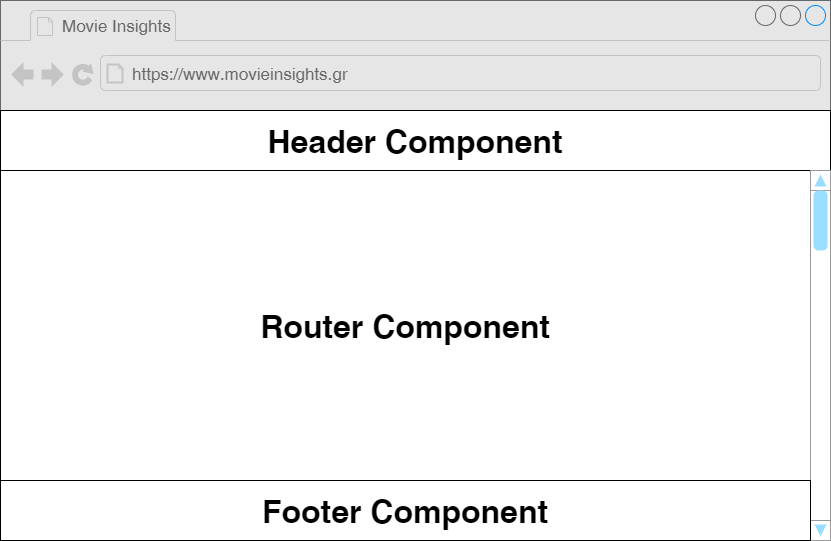
\includegraphics[width=145mm]{Chapters/5 - Architecture/Client/Images/main_struct.png}
  \caption{Βασική διάταξη Web εφαρμογής}
  \label{wire:main}
\end{figure}

Η εφαρμογή αυτή επίσης έχει Modules. Η ένοια Module στην React δεν υπάρχει σε αντιθεση με κάποιο αλλο Web Framework όπως η Angular, αλλα για αυτήν την εφαρμογή στην ουσία ορίζει μια λειτουργία και ομαδοποιεί ολα τα Components αυτής της λειτουργίας μαζί. 

Η αρχιτεκτονική του Router είναι δυναμική καθώς επιτρέπει κάθε module να ορίζει το δικο της Router με τα δικά του Routes. Υπάρχουν 2 ειδών Routes. Το πρώτο είναι το απλο Route που όταν αλλάζει η διεύθυνση στην γραμμή εισαγωγής διεύθυνσης σελίδας αλλάζει και το περιεχόμενο. Το δεύτερο ονομάζεται PrivateRoute και επιτρέπει την πρόσβαση στην δηλωμένη διεύθυνση μόνο αν ο χρήστης έχει κάνει Login, και είναι εξουσιοδοτημένος για να δεί αυτό που ζητάει. 

\subsection{Dashboard Module}
Το Dashboard είναι το κεντρικό Module της εφαρμογής, που φαίνεται και στην αρχική σελίδα και εμφανίζει μέσω του MIDashboard Component 4 διαφορετικά κομμάτια. Το πρώτο κομμάτι είναι η μπάρα αναζήτησης, το δεύτερο κομμάτι είναι ένας παγκόσμιος χάρτης, το τρίτο κομμάτι είναι στα δεξιά του χάρτη και αποτελείται από γραφήματα και συγκεντρωτικά στοιχεία και το τέταρτο και τελευταίο κομμάτι είναι τα κύρια δεδομένα της εφαρμογής όπως ο πιο δημοφιλής ηθοποιός, η ή ταινία με τα μεγαλύτερα έσοδα κ.λ.π όπως φαίνεται στο σχήμα \ref{wire:dashboard}.

\begin{figure}[H]
  \centering
  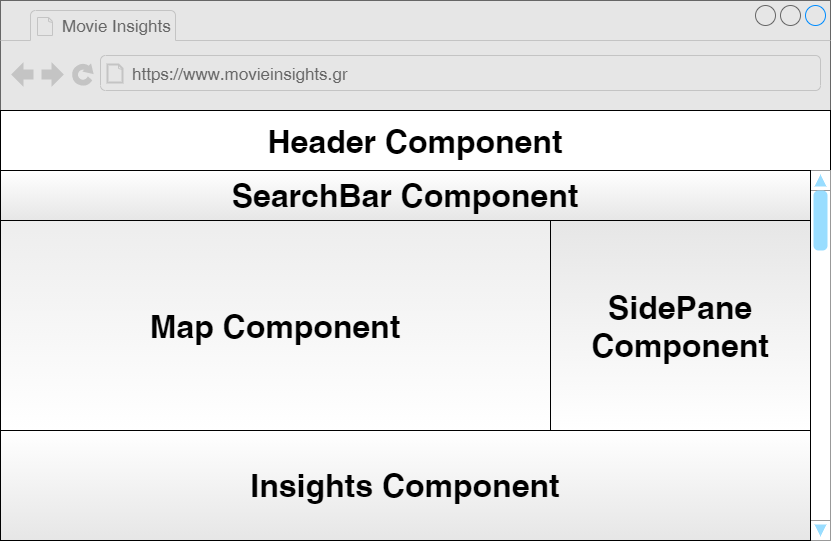
\includegraphics[width=145mm]{Chapters/5 - Architecture/Client/Images/dashboard_struct.png}
  \caption{Βασική διάταξη Web εφαρμογής}
  \label{wire:dashboard}
\end{figure}

Το Dashboard Module ορίζει το δικό του Router που αποτελείται από ένα Route /app/* και ένα RedirectRoute από το κεντρικό Route / στο /app το οποίο είναι η κεντρική σελίδα καθώς δεν χρειάζεται κάτι σύνθετο. 

Ο τρόπος που λειτουργεί είναι ο εξής. Είναι επιλεγμένη για παράδειγμα μια κατηγορία "Στοιχεία για την χώρα Ελλάδα".
Σε αυτήν την κατηγορία στα δεδομένα υπάρχουν οι πιο δημοφιλείς ηθοποιοί, παραγωγοί, σκηνοθέτες, συγγραφείς που έχουν συμμετάσχει σε ταινίες που είτε η παρήγαγε η Ελλάδα είτε η Ελλάδα ήταν χώρα συμπαραγωγής. Αναφέρει επίσης την πιο δημοφιλή εταιρία παραγωγής που συνεργάστηκε η Ελλάδα αλλά και την πιο δημοφιλή χώρα συμπαραγωγής και είδος ταινίας. Επιπρόσθετα αναφέρει τα μέσα και συνολικά έσοδα/έξοδα καθώς και το καθαρό κέρδος. Όλα αυτά τα στοιχεία υπάρχουν επίσης και ανά χρόνο, για όσα χρόνια υπάρχουν στην βάση δεδομένων για την Ελλάδα. Όλες οι κατηγορίες λειτουργούν με τον ίδιο τρόπο με την εξαίρεση της κατηγορίας ανά άτομο. Που εκεί εκτός από την επιλογή χρόνου, υπάρχει και η επιλογή ρόλου, με διαθέσιμους ρόλους: ηθοποιός, σκηνοθέτης, συγγραφέας και παραγωγός. Για τα άτομα υπάρχουν συγκεντρωτικά στοιχεία μόνο ανά ρόλο και όχι συνολικά, καθώς είναι διαφορετικά τα δεδομένα. Πάραυτα όλα τα στοιχεία ανά ρόλο υπάρχουν και ανά χρόνο.

Το Dashboard Module περιέχει μόνο ένα Component το ΜΙDashboard Component. Όλα τα δεδομένα που υπολογίζονται μέσα από το Dashboard Module στέλνονται απευθείας στο ΜΙDashboard Component.

Μέσω των Component που δηλώνονται και δομείται όλη η εφαρμογή καθίσταται εφικτή η πλοήγηση σε όλο το εύρος των δεδομένων της εφαρμογής. Ενώ θα μπορούσε σε κάθε Component, που επηρεάζει τα δεδομένα που εμφανίζονται, να υλοποιηθεί η λογική της αλλαγής των δεδομένων, προτιμήθηκε όλα αυτά τα Component απλά να αλλάζουν την διεύθυνση στην γραμμή διεύθυνσης του Browser και με βάση την διεύθυνση που άλλαξε χωρίς να γίνεται ανακατεύθυνση το Dashboard Module καταλαβαίνει τι χρειάζεται να αλλάξει, αλλάζει τα δεδομένα μέσω του Redux State Manager, και ύστερα στέλνει τα δεδομένα σε όλα τα επιμέρους Components για να αλλάξουν. Ενώ ακούγεται πιο σύνθετη τεχνική, χρησιμοποιήθηκε για την ευκολία διαχείρισης και συντήρησης του κώδικα, καθώς στην άλλη περίπτωση θα έπρεπε σε περίπτωση αλλαγής του κώδικα εμφάνισης των δεδομένων, να πραγματοποιηθούν αλλαγές σε κάθε Component που άλλαζε δεδομένα. Ενώ με αυτήν την υλοποίηση τα πάντα βρίσκονται σε ένα μέρος. Ένας ακόμα σημαντικός λόγος που προτιμήθηκε η συγκεκριμένη τεχνική είναι η προσβασιμότητα στα δεδομένα αυτά. Λόγω της φύσης της αρχιτεκτονικής της εφαρμογής και όντας SPA, υπάρχει ουσιαστικά μόνο μια αληθινή σελίδα που είναι προσβάσιμη από έναν Browser. Αυτή είναι η index.html που είναι ένα αρχείο HTML το οποίο φορτώνει όλον τον κώδικα της εφαρμογής. Χωρίς την αλλαγή της διεύθυνσης, ένας χρήστης θα έπρεπε να μπει στην αρχική σελίδα και να εκτελέσει κάποιες ενέργειες έτσι ώστε να φτάσει στο ίδιο σημείο που βρισκόταν πριν. Με την αλλαγή της διεύθυνσης όμως, όχι μόνο μπορεί να επανέλθει στο σημείο στο οποίο βρισκόταν αλλά μπορεί και να μοιραστεί τον σύνδεσμο με κάποιον άλλον χρήστη και να κοιτάνε τα ίδια δεδομένα. 

Το Dashboard Module λοιπόν παρακολουθεί τις αλλαγές διευθύνσεων που γίνονται μετά την βασική διεύθυνση /app/ και με την χρήση κάποιον βοηθητικών συναρτήσεων αλλάζει τα δεδομένα όπως φαίνεται στον κώδικα \ref{code:urlIntercept}.

\begin{figure}[h]
    \begin{TypeScriptcode}
handleViewChange = () => {
    const path = this.props.location.pathname;
    if (this.state.path !== path || !this.state.pathHandled) {
      if (!this.state.pathHandled) {
        let pathMatch: match;
        if ((pathMatch = matchPath(path, "/app/:entity(country|company|genre)/:id-:name/:year(\\d{4})?"))) {
          this.handleGenericChange(pathMatch.params['entity'], +pathMatch.params['id'], +pathMatch.params['year']);
        } else if ((pathMatch = matchPath(path, "/app/person/:id-:name/:role([A-z]+)?/:year(\\d{4})?"))) {
          this.handlePersonChange(+pathMatch.params['id'], +pathMatch.params['year'], pathMatch.params['role']);
        } else if ((pathMatch = matchPath(path, "/app/:general(general)?/:year(\\d{4})?"))) {
          this.handleGeneralChange(+pathMatch.params['year']);
        }
        this.scrollElement();
        if (this.state.path !== path)
          this.setState({path});
      }
      if (this.state.path !== path) {
        this.setState({pathHandled: false});
      }
    }
}
    \end{TypeScriptcode}
    \caption{Αλγόριθμος παρακολούθησης αλλαγής στην γραμμή διευθύνσεων ενός Browser.}
   \label{code:urlIntercept}
\end{figure}

Η αλλαγή της διεύθυνσης στην γραμμή διευθύνσεων του Browser, δημιουργείται από μια βοηθητική συνάρτηση όπως φαίνεται στον κώδικα \ref{code:urlBuilder}. Με αυτόν τον τρόπο όλα τα Components που έχουν ως σκοπό την αλλαγή των δεδομένων μπορούν να αλλάξουν εύκολα την διεύθυνση χρησιμοποιώντας αυτήν την συνάρτηση, και αν αλλάξει ποτέ η δομή της διεύθυνσης η αλλαγή θα γίνει μόνο μέσα σε αυτήν την συνάρτηση διευκολύνοντας παράλληλα την συντήρηση και την αντιμετώπιση προβλημάτων του κώδικα.

\begin{figure}[h]
    \begin{TypeScriptcode}
function |$\textbf{generateNavigationLink}$|(entity?: BaseNamedEntity, role?: CreditRole, year?: number, entityType?: EntityType) {
  let type = undefined;
  if (entity) {
    if (entityType) {
      type = entityType.toLowerCase();
    } else if (isMovie(entity)) {
      type = 'movie';
    } else if (isPerson(entity)) {
      type = 'person';
    } else if (isCompany(entity)) {
      type = 'company';
    } else if (isCountry(entity)) {
      type = 'country';
    } else if (isGenre(entity)) {
      type = 'genre';
    }
  } else if (year) {
    type = 'general';
  }
  return `/app${type ? `/${type}` : ''}${entity ? `/${entity.id}-${normalizeText(entity.name)}` : ''}${role && type === 'person' ? `/${role}` : ''}${year ? `/${year}` : ''}`;
}
    \end{TypeScriptcode}
    \caption{Αλγόριθμος δημιουργίας διεύθυνσης αλλαγής δεδομένων.}
   \label{code:urlBuilder}
\end{figure}

Το Redux State Manager χρησιμοποιήθηκε για 2 λόγους. Προσφέρει μια εύκολη διεπαφή που βασίζεται στο Immutability των δεδομένων συμβάλλοντας δραστικά στην μείωση των Side Effects, αλλά επίσης χρησιμοποιήθηκε σαν ένα Facade για την απόκτηση των δεδομένων από την υπηρεσία.

Γνωρίζοντάς ότι οποιαδήποτε ενέργεια εμπεριέχει κάποιου είδους επικοινωνία με μια εξωτερική υπηρεσία αυξάνει σημαντικά τον χρόνο της διεκπεραίωσης της, και έχοντας σαν δεδομένο ότι η JavaScript που τρέχει μέσα σε έναν Browser τρέχει σε ένα και μοναδικό νήμα (Thread), η εμπειρία του χρήστη θα ήταν πολύ άσχημη όταν θα ζητούσε νέα δεδομένα από τον Server, καθώς η Web Εφαρμογή θα ήταν μη αποκρίσιμη για αρκετό διάστημα μέχρι την απόκτηση των δεδομένων και την εμφάνιση τους. Για αυτόν τον λόγο χρησιμοποιήθηκε ένα πρόσθετο στο Redux Fraemwork, που επιτρέπει την ασύγχρονη απόκτηση δεδομένων και την αποθήκευση τους στο κεντρικό State της εφαρμογής. Όλα τα Components που εξαρτιούνται από αυτό το Global State, όταν αλλάξει θα αλλάξουν και αυτά τα δεδομένα που εμφανίζουν.

Όπως προαναφέρθηκε το Dashboard Component περιέχει 4 σημαντικά Component που εμφανίζουν όλα τα απαραίτητα δεδομένα.

\input{Chapters/5 - Architecture/Client/SearchbarComponent/Main}
\input{Chapters/5 - Architecture/Client/MapComponent/Main}
\input{Chapters/5 - Architecture/Client/SidePaneComponent/Main}
\input{Chapters/5 - Architecture/Client/InsightsComponent/Main}
\subsection{Admin Module}
Το Admin Module είναι ένα σύνολο λειτουργιών που επιτρέπει έναν διαχειριστή να διαχειρίζεται με ευκολία την εφαρμογή. Στην παρούσα υλοποίηση το Admin Module έχει 2 διαφορετικές σελίδες - Components, το Κέντρο Ελέγχου και το Κέντρο Διαχείρισης Καταγραφών. Για να αποκτήσει πρόσβαση ένας χρήστης στις λειτουργίες του Admin Module, πρέπει να έχει κάνει Login και να είναι εξουσιοδοτημένος με τον ρόλο ADMIN, διαχειριστή. 

Το Κέντρο Ελέγχου είναι μια σελίδα που επιτρέπει την παρακολούθηση της κατάστασης της υγείας της εφαρμογής, προσφέρει στατιστικά των υπηρεσιών αλλά και του λειτουργικού που τρέχει η εφαρμογή αλλα παράλληλα προσφέρει και διαγνωστικά για να γνωρίζει ο διαχειριστής τι γίνεται ανά πάσα στιγμή στην εφαρμογή αυτήν όπως φαίνεται στις εικόνες \ref{layout:admin_cc_1} και \ref{layout:admin_cc_2}. 

Αποτελείται από πολλά διαφορετικά Components τα οποία ενημερώνονται ανάλογα με τον τύπο των δεδομένων που προσφέρουν ανά μισό, δύο και ανά πέντε δευτερόλεπτα με την χρήση WebSockets μέσο του Spring Boot Actuator έτσι ώστε η εικόνα που βλέπει ο διαχειριστής να αντικατοπτρίζει πάντα την κατάσταση της εφαρμογής εκείνη την χρονική στιγμή.

Το Κέντρο Διαχείρισής Καταγραφών είναι στην ουσία ένας διαδραστικός πίνακας που επιτρέπει στον διαχειριστή να αλλάζει τα επίπεδα καταγραφής διάφορων υπηρεσιών μέσα στον Server. Τα επίπεδα καταγραφής ορίζουν τι πληροφορίες θα δίνει η κάθε υπηρεσία. Το επίπεδο καταγραφής ERROR για παράδειγμα καταγράφει μόνο τα μηνύματα σφαλμάτων στο αρχείο καταγραφής της υπηρεσίας, ενώ το επίπεδο καταγραφής WARNING καταγράφει και τα μηνύματα σφαλμάτων αλλά και τα μηνύματα προειδοποιήσεων. Αυτό είναι πολύ χρήσιμο όταν χρησιμοποιείται σε συνδυασμό με μια υπηρεσία διαχείρισης καταγραφών όπως η Logstash για παράδειγμα. Με αυτόν τον τρόπο ο διαχειριστής δεν χρειάζεται να έχει φυσική πρόσβαση στο μηχάνημα που τρέχει την εφαρμογή για να μπορεί να δει τα αρχεία καταγραφής παρά μόνο να μπει στην υπηρεσία διαχείρισης καταγραφών και να βρει ότι χρειάζεται από εκεί.

Ο πίνακας του Κέντρου Διαχείρισής Καταγραφών φαίνεται στην εικόνα \ref{layout:admin_l}. Η συγκεκριμένη εικόνα τραβήχτηκε κατά την ανάπτυξη της εφαρμογής και δείχνει ότι το κεντρικό επίπεδο καταγραφών ROOT είναι ορισμένο στο DEBUG που σημαίνει ότι καταγράφει ακόμα και μηνύματα διαγνωστικών με κάποιες εξαιρέσεις που έχουν οριστεί σε επίπεδο WARNING για να μην υπερφορτώσουν τα αρχεία καταγραφής με περιττές πληροφορίες.

\begin{figure}[H]
  \centering
  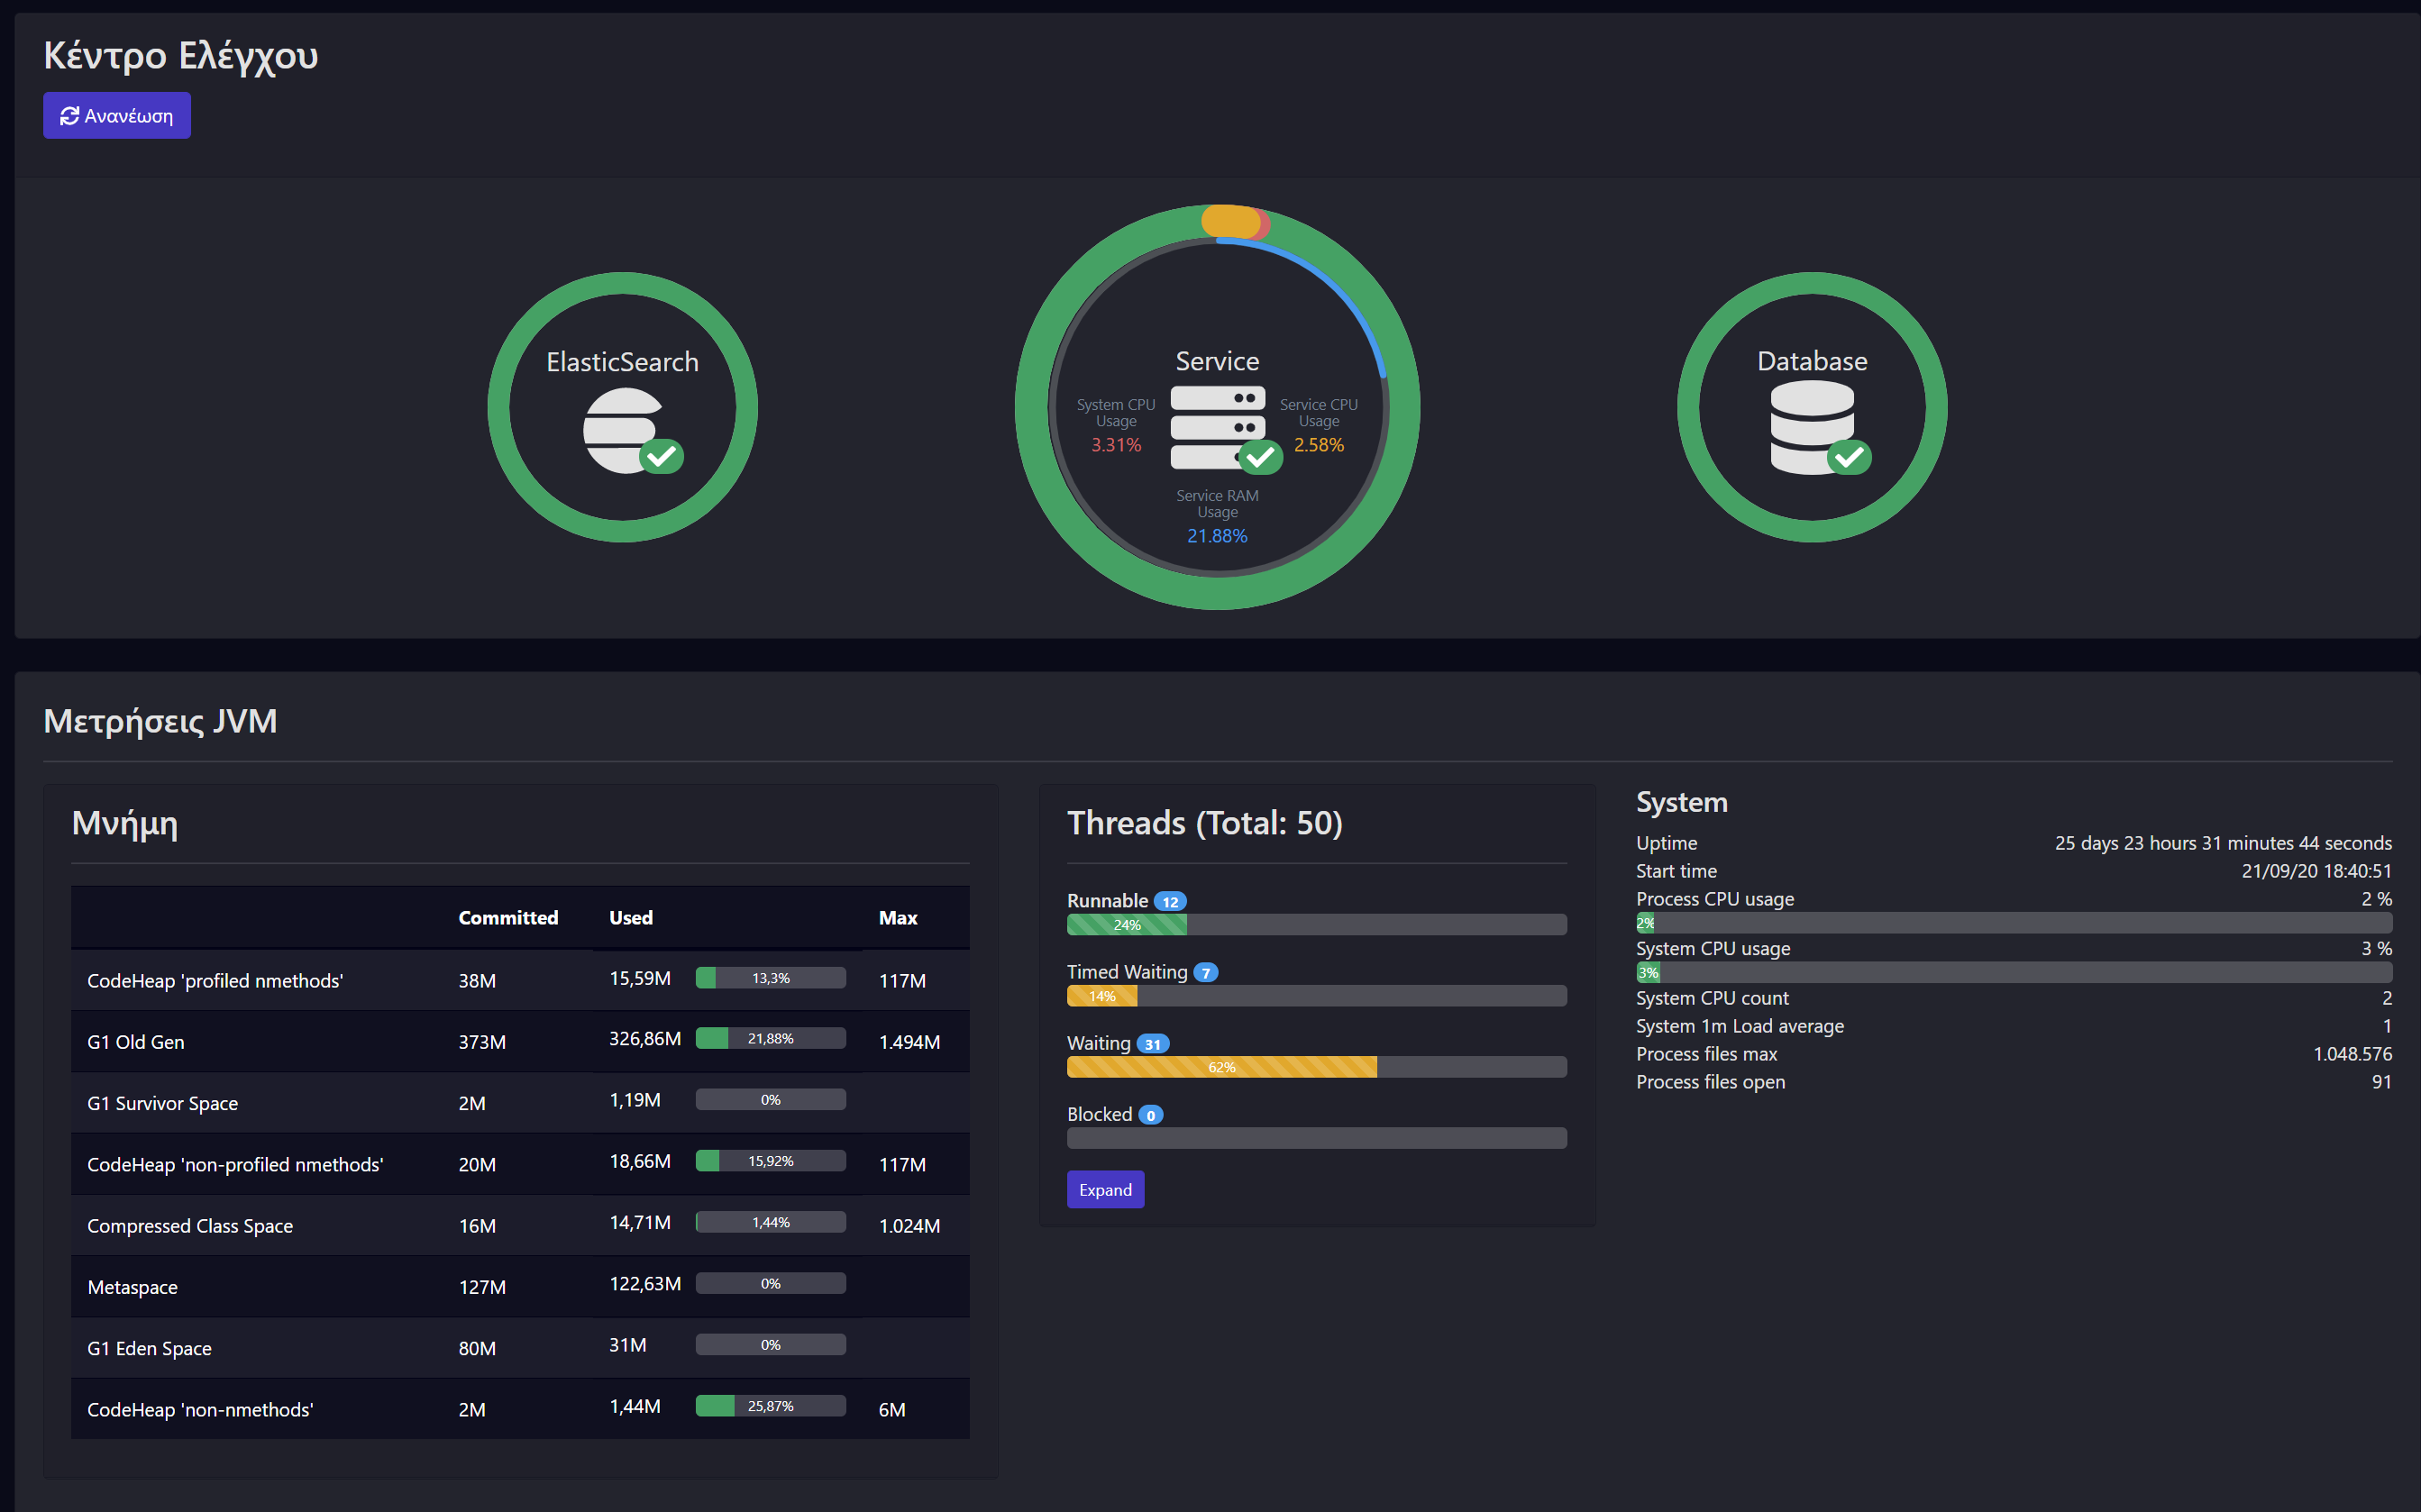
\includegraphics[width=145mm]{Chapters/5 - Architecture/Client/Images/admin_control_center.png}
  \caption{Κέντρο Ελέγχου}
  \label{layout:admin_cc_1}
\end{figure}
\begin{figure}[H]
  \centering
  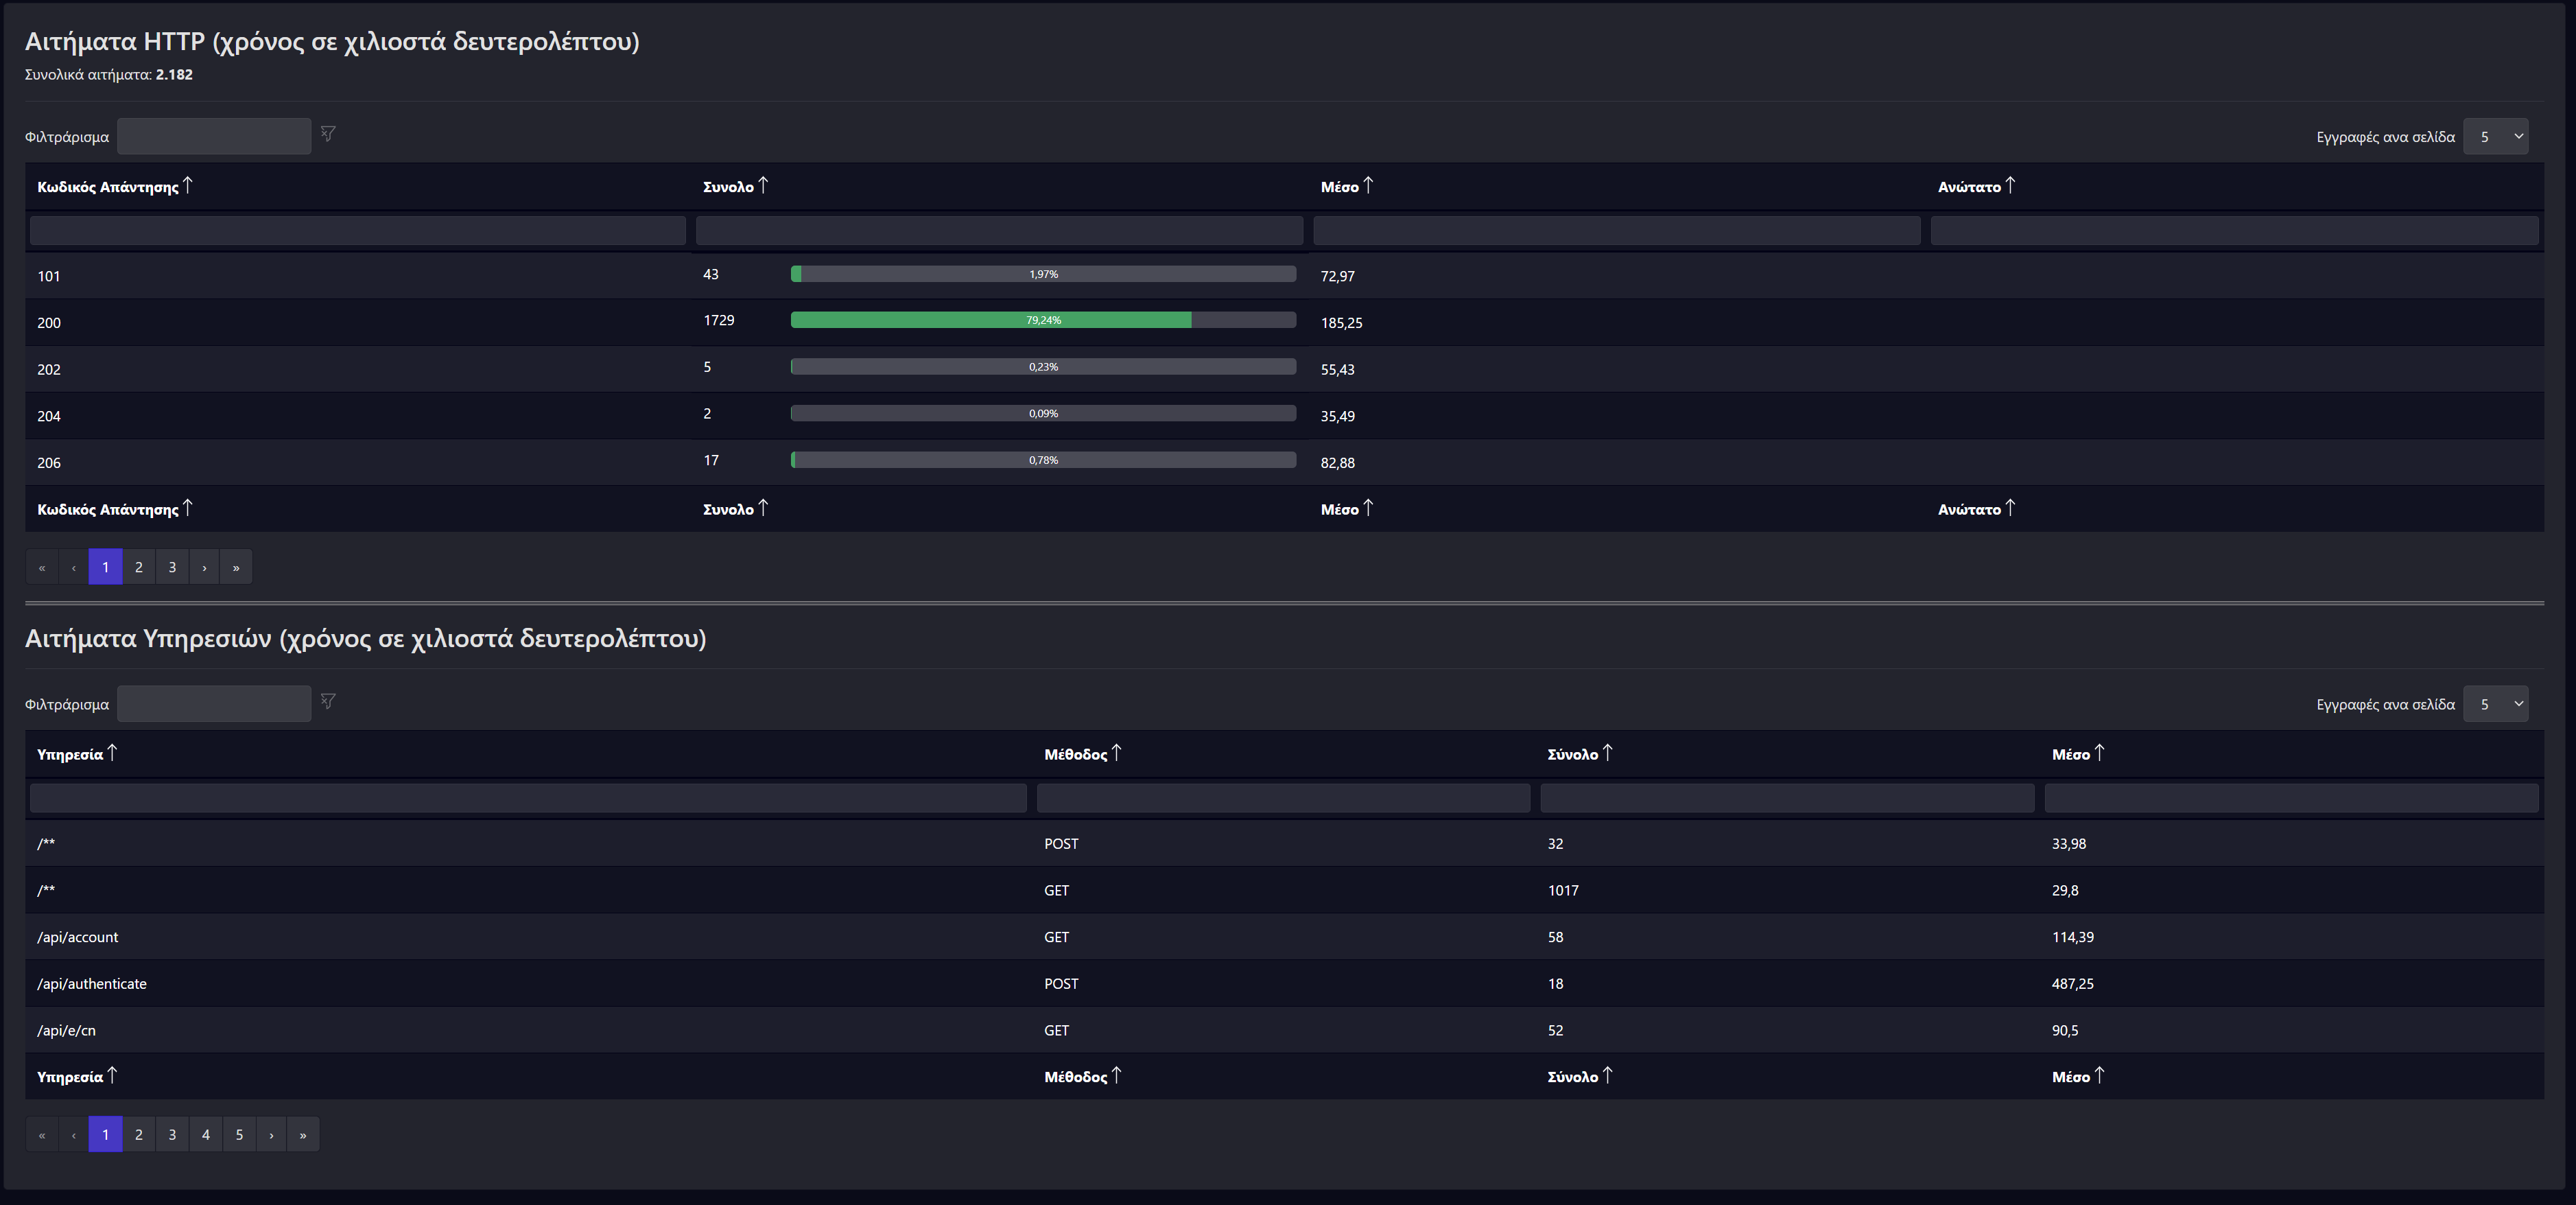
\includegraphics[width=145mm]{Chapters/5 - Architecture/Client/Images/admin_control_center_2.png}
  \caption{Κέντρου Ελέγχου - συνέχεια}
  \label{layout:admin_cc_2}
\end{figure}
\begin{figure}[H]
  \centering
  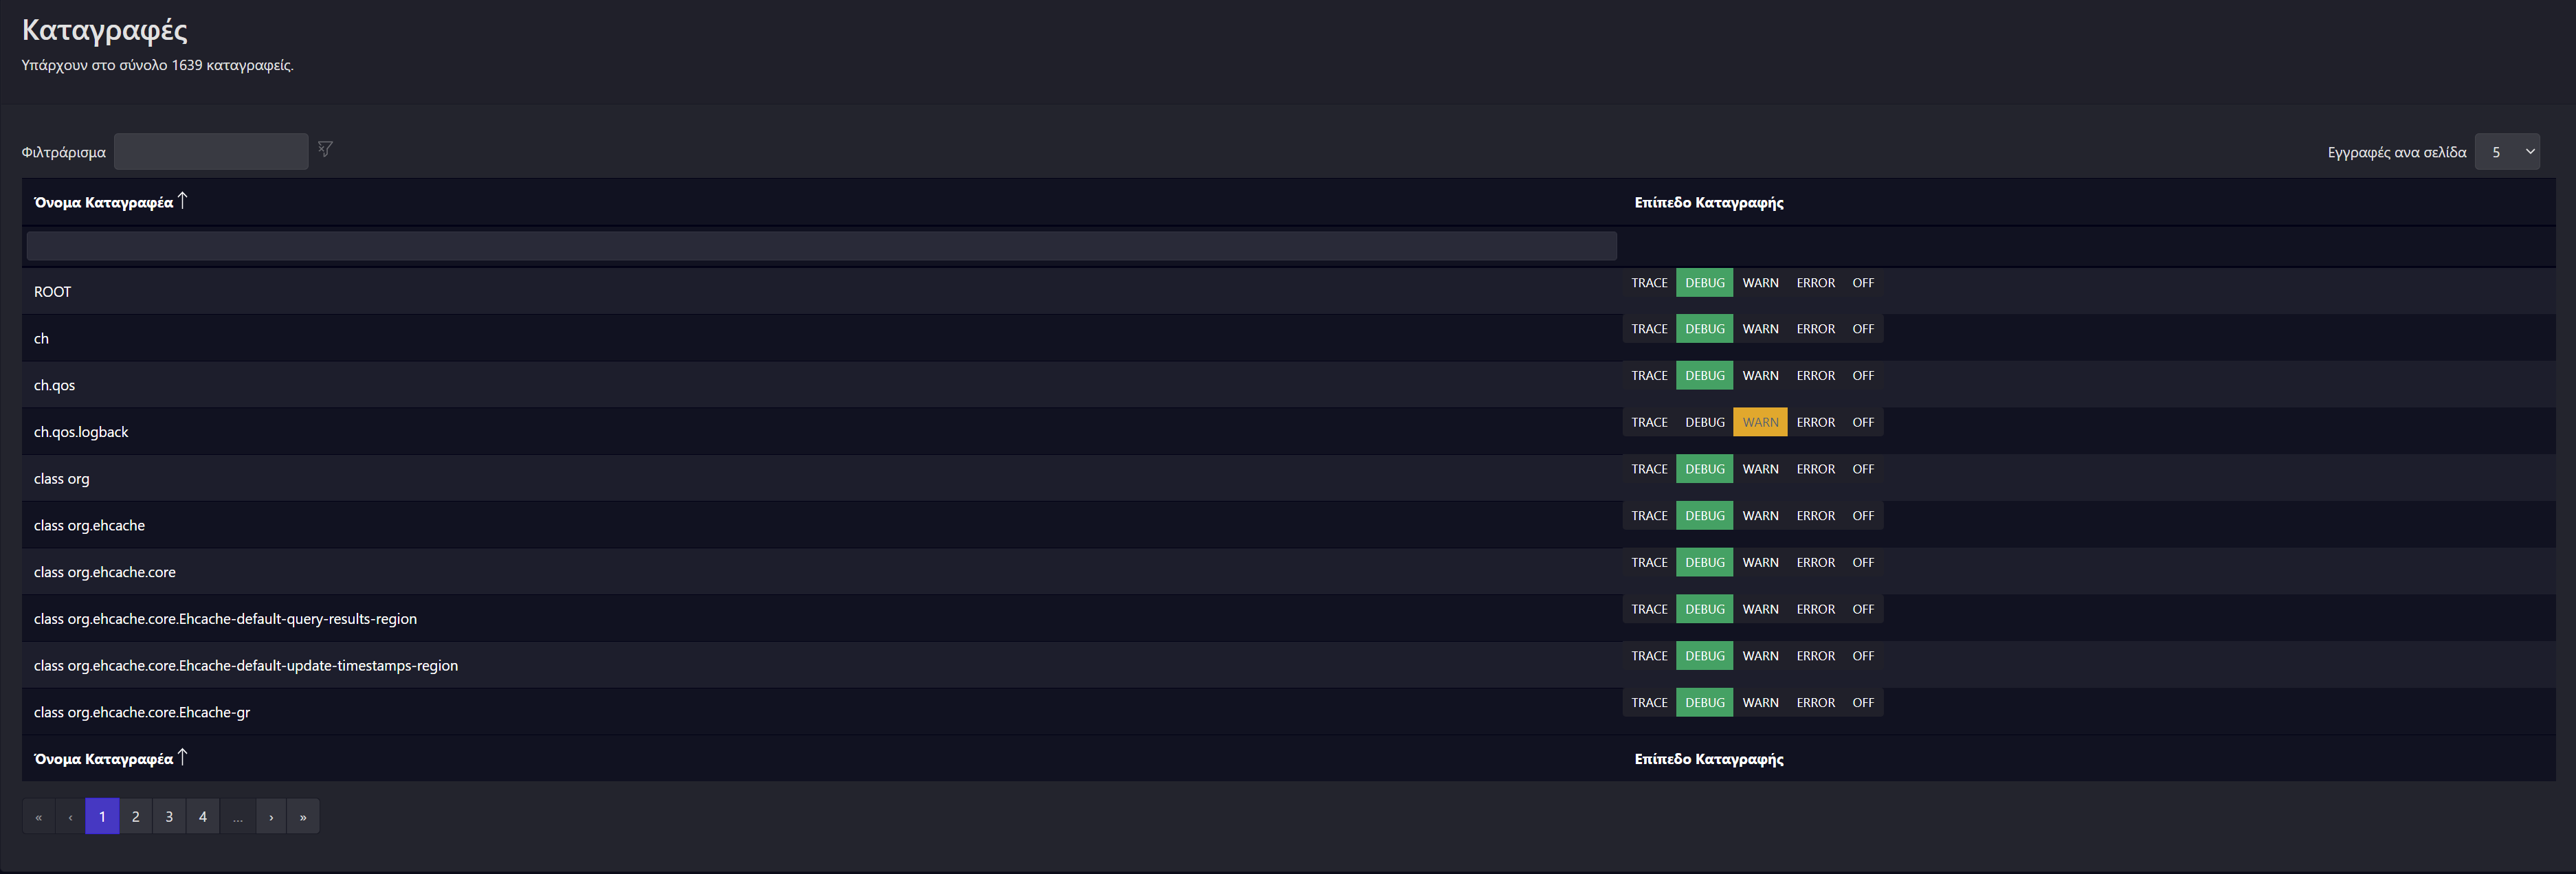
\includegraphics[width=145mm]{Chapters/5 - Architecture/Client/Images/admin_l.png}
  \caption{Κέντρο Διαχείρισής Καταγραφών}
  \label{layout:admin_l}
\end{figure}
\chapter{Εγχειρίδιο Χρήσης}
Παρακάτω παρατίθεται ένα αναλυτικό εγχειρίδιο χρήσης για το πως μπορεί να χρησιμοποιηθεί η εφαρμογή αυτή από κάθε χρήστη.

Αρχικά ο χρήστης πρέπει να ανοίξει έναν φυλλομετρητή (Browser) και να πλοηγηθεί στην σελίδα http://www.movieinsights.gr/ . Η Αρχική σελίδα που θα μπει είναι και ουσιαστικά όλη η εφαρμογή. Η πρώτη κατηγορία που θα εμφανιστεί με το που θα μπει ο χρήστης στην εφαρμογή είναι η κατηγορία των γενικών στοιχείων.

Η κατηγορία των γενικών στοιχείων περιέχει στοιχεία συγκεντρωτικά για όλες τις ταινίες, τους ηθοποιούς, τις εταιρίες παραγωγής, τις χώρες παραγωγής αλλά και τα είδη παραγωγής που υπάρχουν στην βάση δεδομένων της εφαρμογής. Αυτή η κατηγορία είναι η Παγκόσμια όπως φαίνεται στην εικόνα \ref{demo:main}

\begin{figure}[H]
  \centering
  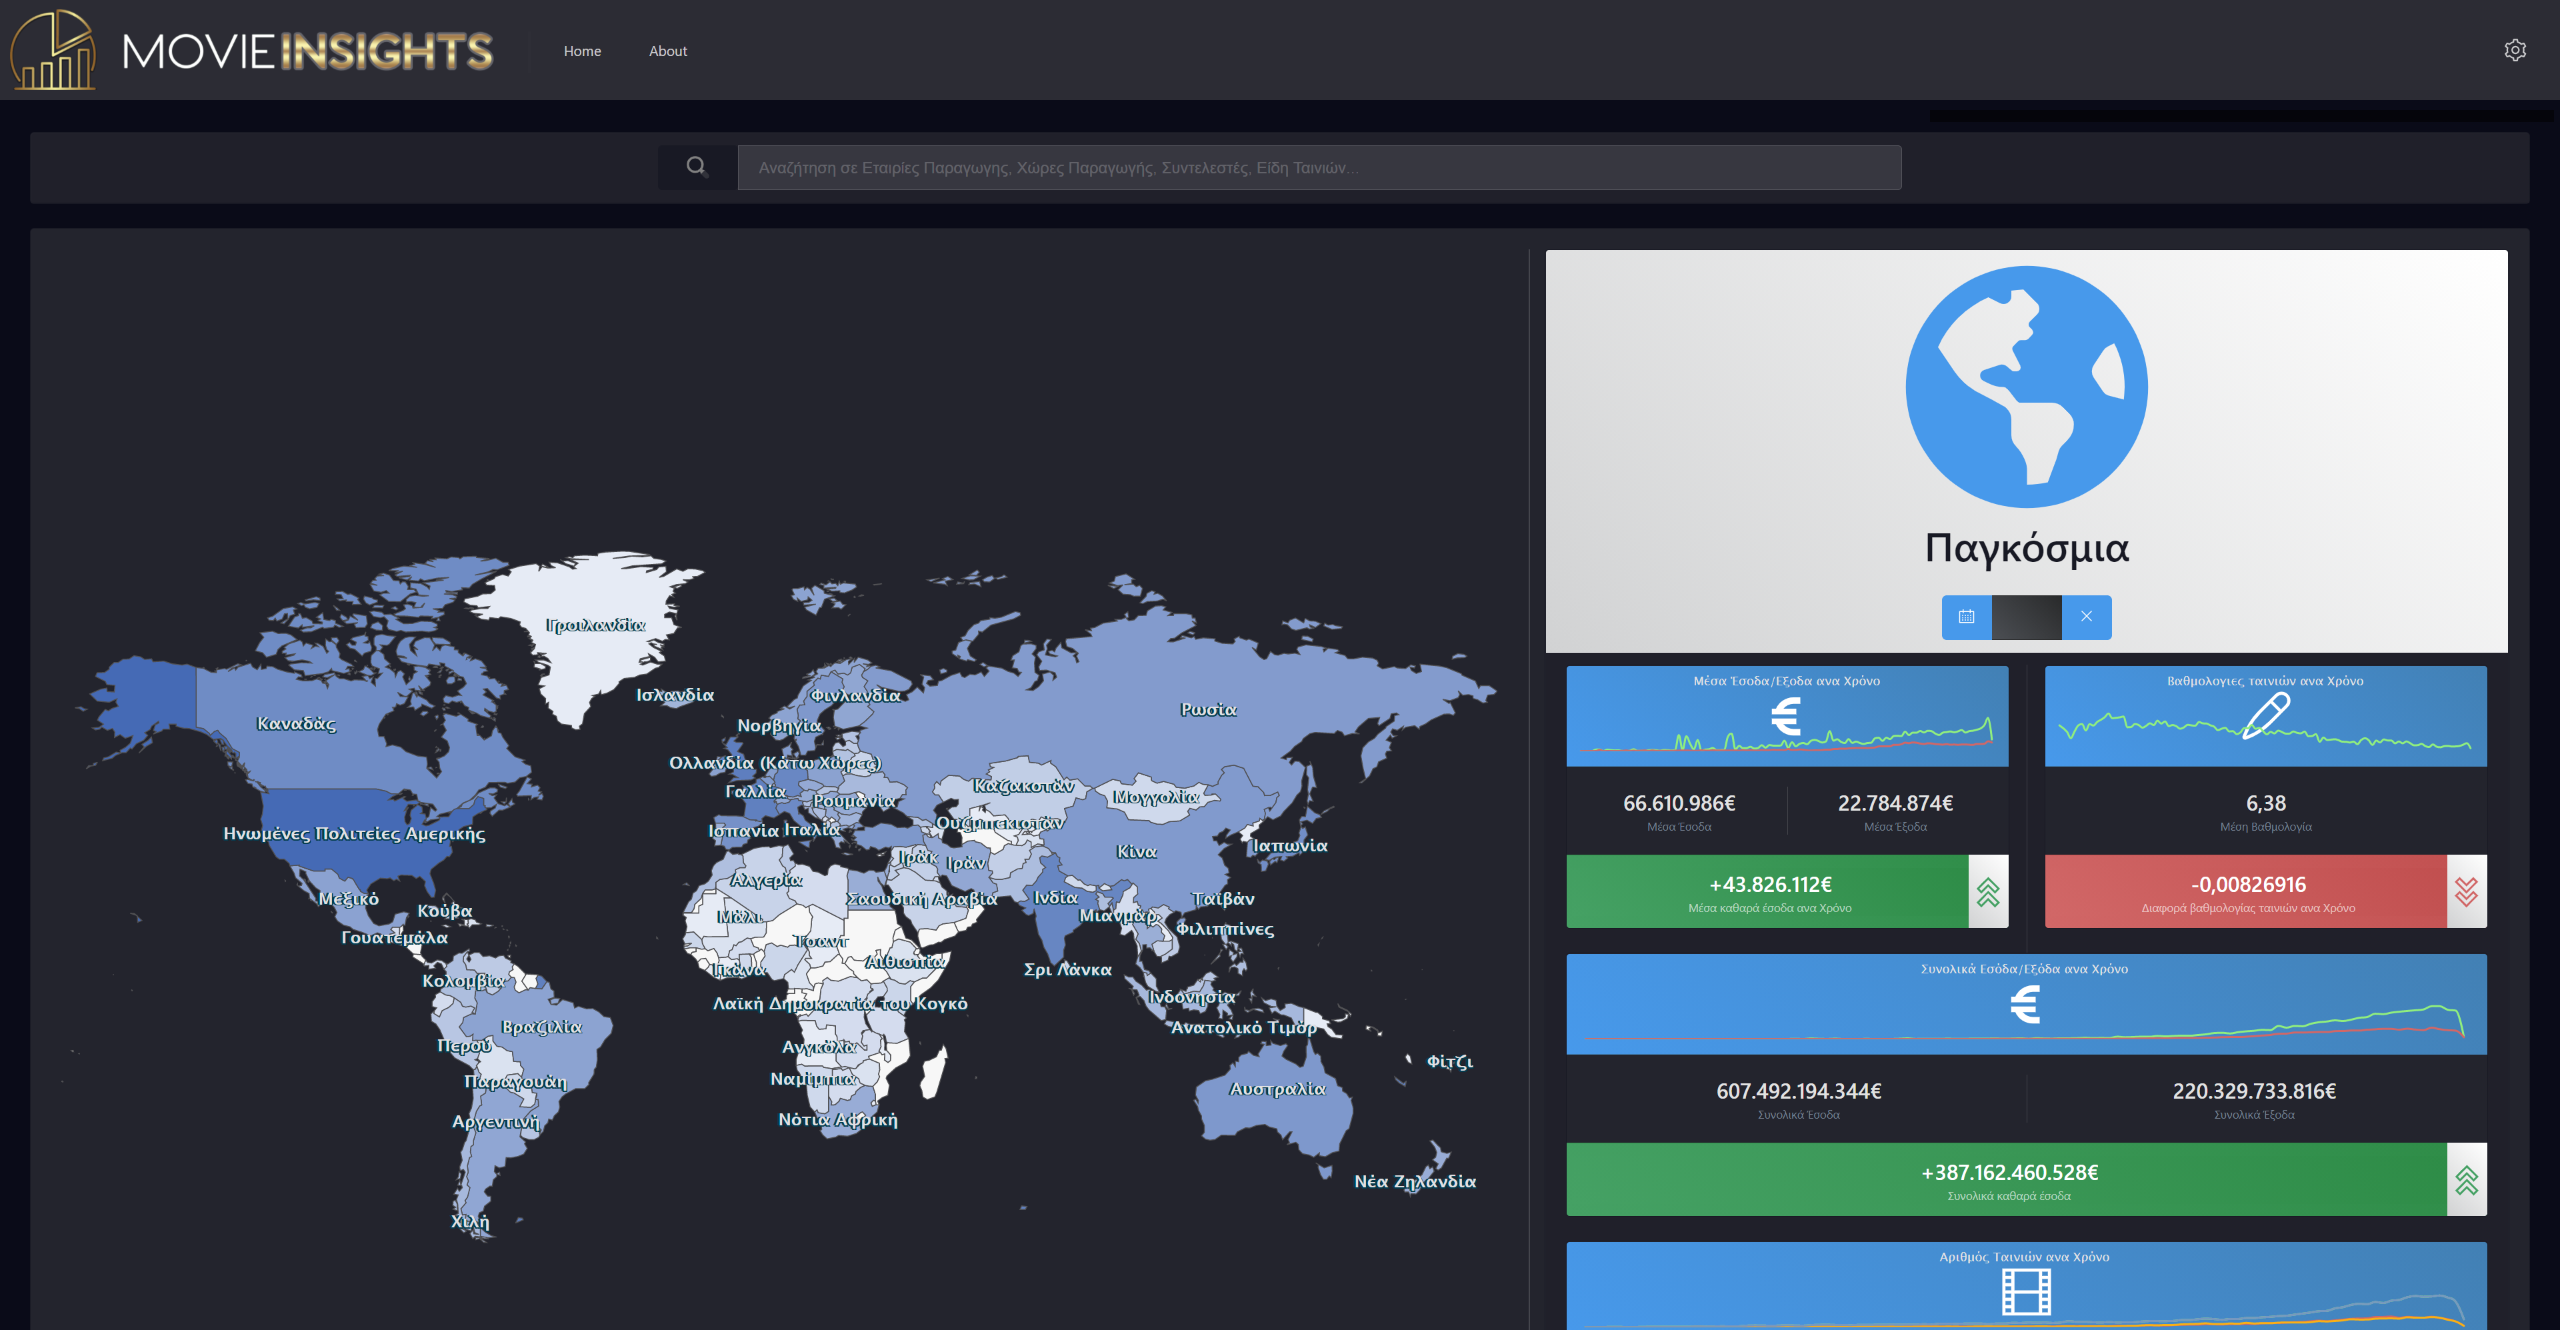
\includegraphics[width=145mm]{Chapters/6 - Manual/Images/main_page.png}
  \caption{Αρχική σελίδα}
  \label{demo:main}
\end{figure}

\section{Μηχανή Αναζήτησης}
Ο χρήστης στην κορυφή της ιστοσελίδας θα βρει μια μπάρα αναζήτησης που του επιτρέπει να ψάξει άτομα, εταιρίες, χώρες και είδη ταινιών. Σε κάθε γράμμα που θα πληκτρολογήσει θα του εμφανίζονται ανάλογα αποτελέσματα για να επιλέξει. Ένα αποτέλεσμα αποτελείται από μια φωτογραφία και έναν τίτλο. Για παράδειγμα αν το αποτέλεσμα είναι μια χώρα η εικόνα θα είναι η σημαία της χώρας και ο τίτλος, το όνομα της. Αν το αποτέλεσμα είναι ένα άτομο η εικόνα θα είναι μια φωτογραφία του ατόμου αν υπάρχει, αλλιώς μια προκαθορισμένη φωτογραφία, και το όνομα του. Αν είναι είδος ταινίας θα υπάρχει ένα εικονίδιο για εικόνα και το όνομα του είδους. Και αν είναι εταιρία το λογότυπο της εταιρίας αν υπάρχει, αλλιώς ένα προκαθορισμένο εικονίδιο κτηρίου όπως φαίνεται στην εικόνα \ref{demo:searchbar} στο 2ο αποτέλεσμα των εταιριών, και το όνομα της. Ο χρήστης πρέπει να επιλέξει ένα από τα προτεινόμενα αποτελέσματα καθώς η γενική αναζήτησης με το πλήκτρο "Enter" δεν υποστηρίζεται.

\begin{figure}[H]
  \centering
  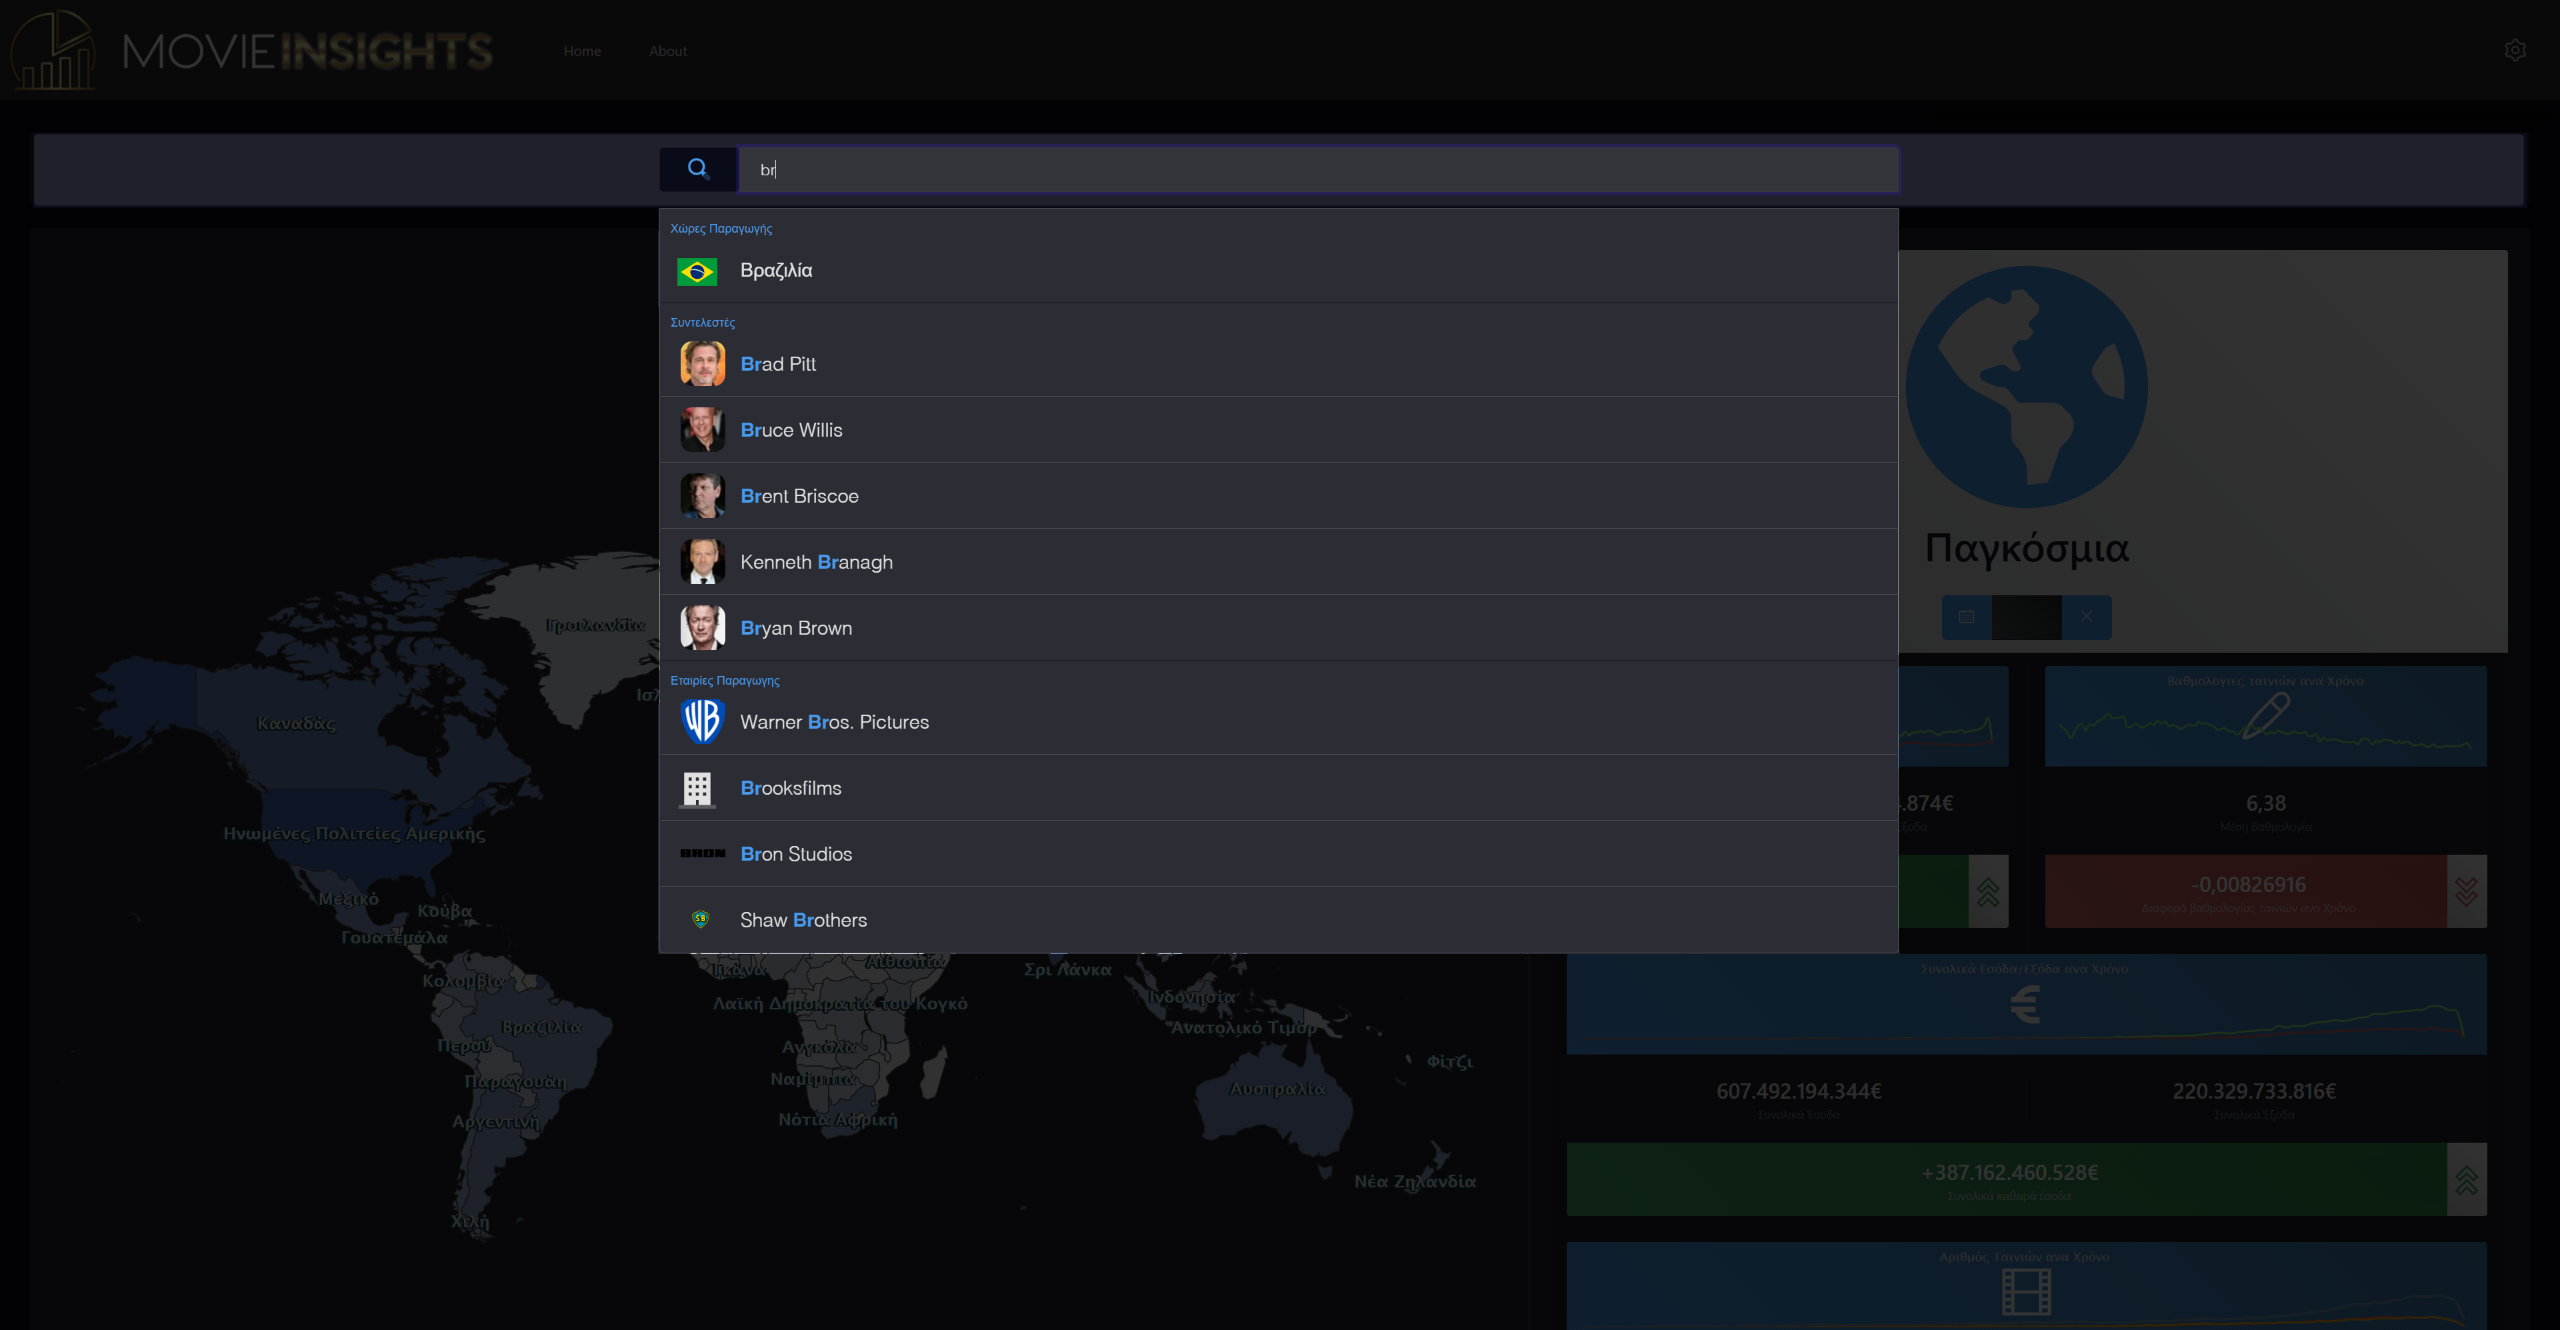
\includegraphics[width=145mm]{Chapters/6 - Manual/Images/main_page_searchbar.png}
  \caption{Γραμμή Αναζήτησης}
  \label{demo:searchbar}
\end{figure}
\section{Χάρτης}
Ακριβώς από κάτω από την μπάρα αναζήτησης βρίσκεται στα αριστερά ένας παγκόσμιος χάρτης ο οποίος έχει δεδομένα για όλες τις χώρες οι οποίες έχουν παράξει έστω και μια ταινία και βρίσκονται φυσικά στην βάση δεδομένων της εφαρμογής.
Οι χώρες στον χάρτη χρωματίζονται από διαφορετικές αποχρώσεις του μπλε, όσο πιο έντονο είναι το χρώμα τόσες παραπάνω ταινίες έχει αυτή η χώρα. Ο Χάρτης υποστηρίζει μεγέθυνσή και κύλιση. Αν ο χρήστης μετακινήσει τον κένσορα του ποντικιού πάνω από μια χώρα ένα βοηθητικό παραθυράκι θα εμφανιστεί από πάνω αναγράφοντας το όνομα της χώρα και το πόσες ταινίες έχει όπως φαίνεται στη εικόνα \ref{demo:map}. Ο χρωματισμός και τα δεδομένα του χάρτη παραμένουν τα ίδια ανεξάρτητα απο την κατηγορία ή το έτος που έχει επιλεγεί.

\begin{figure}[H]
  \centering
  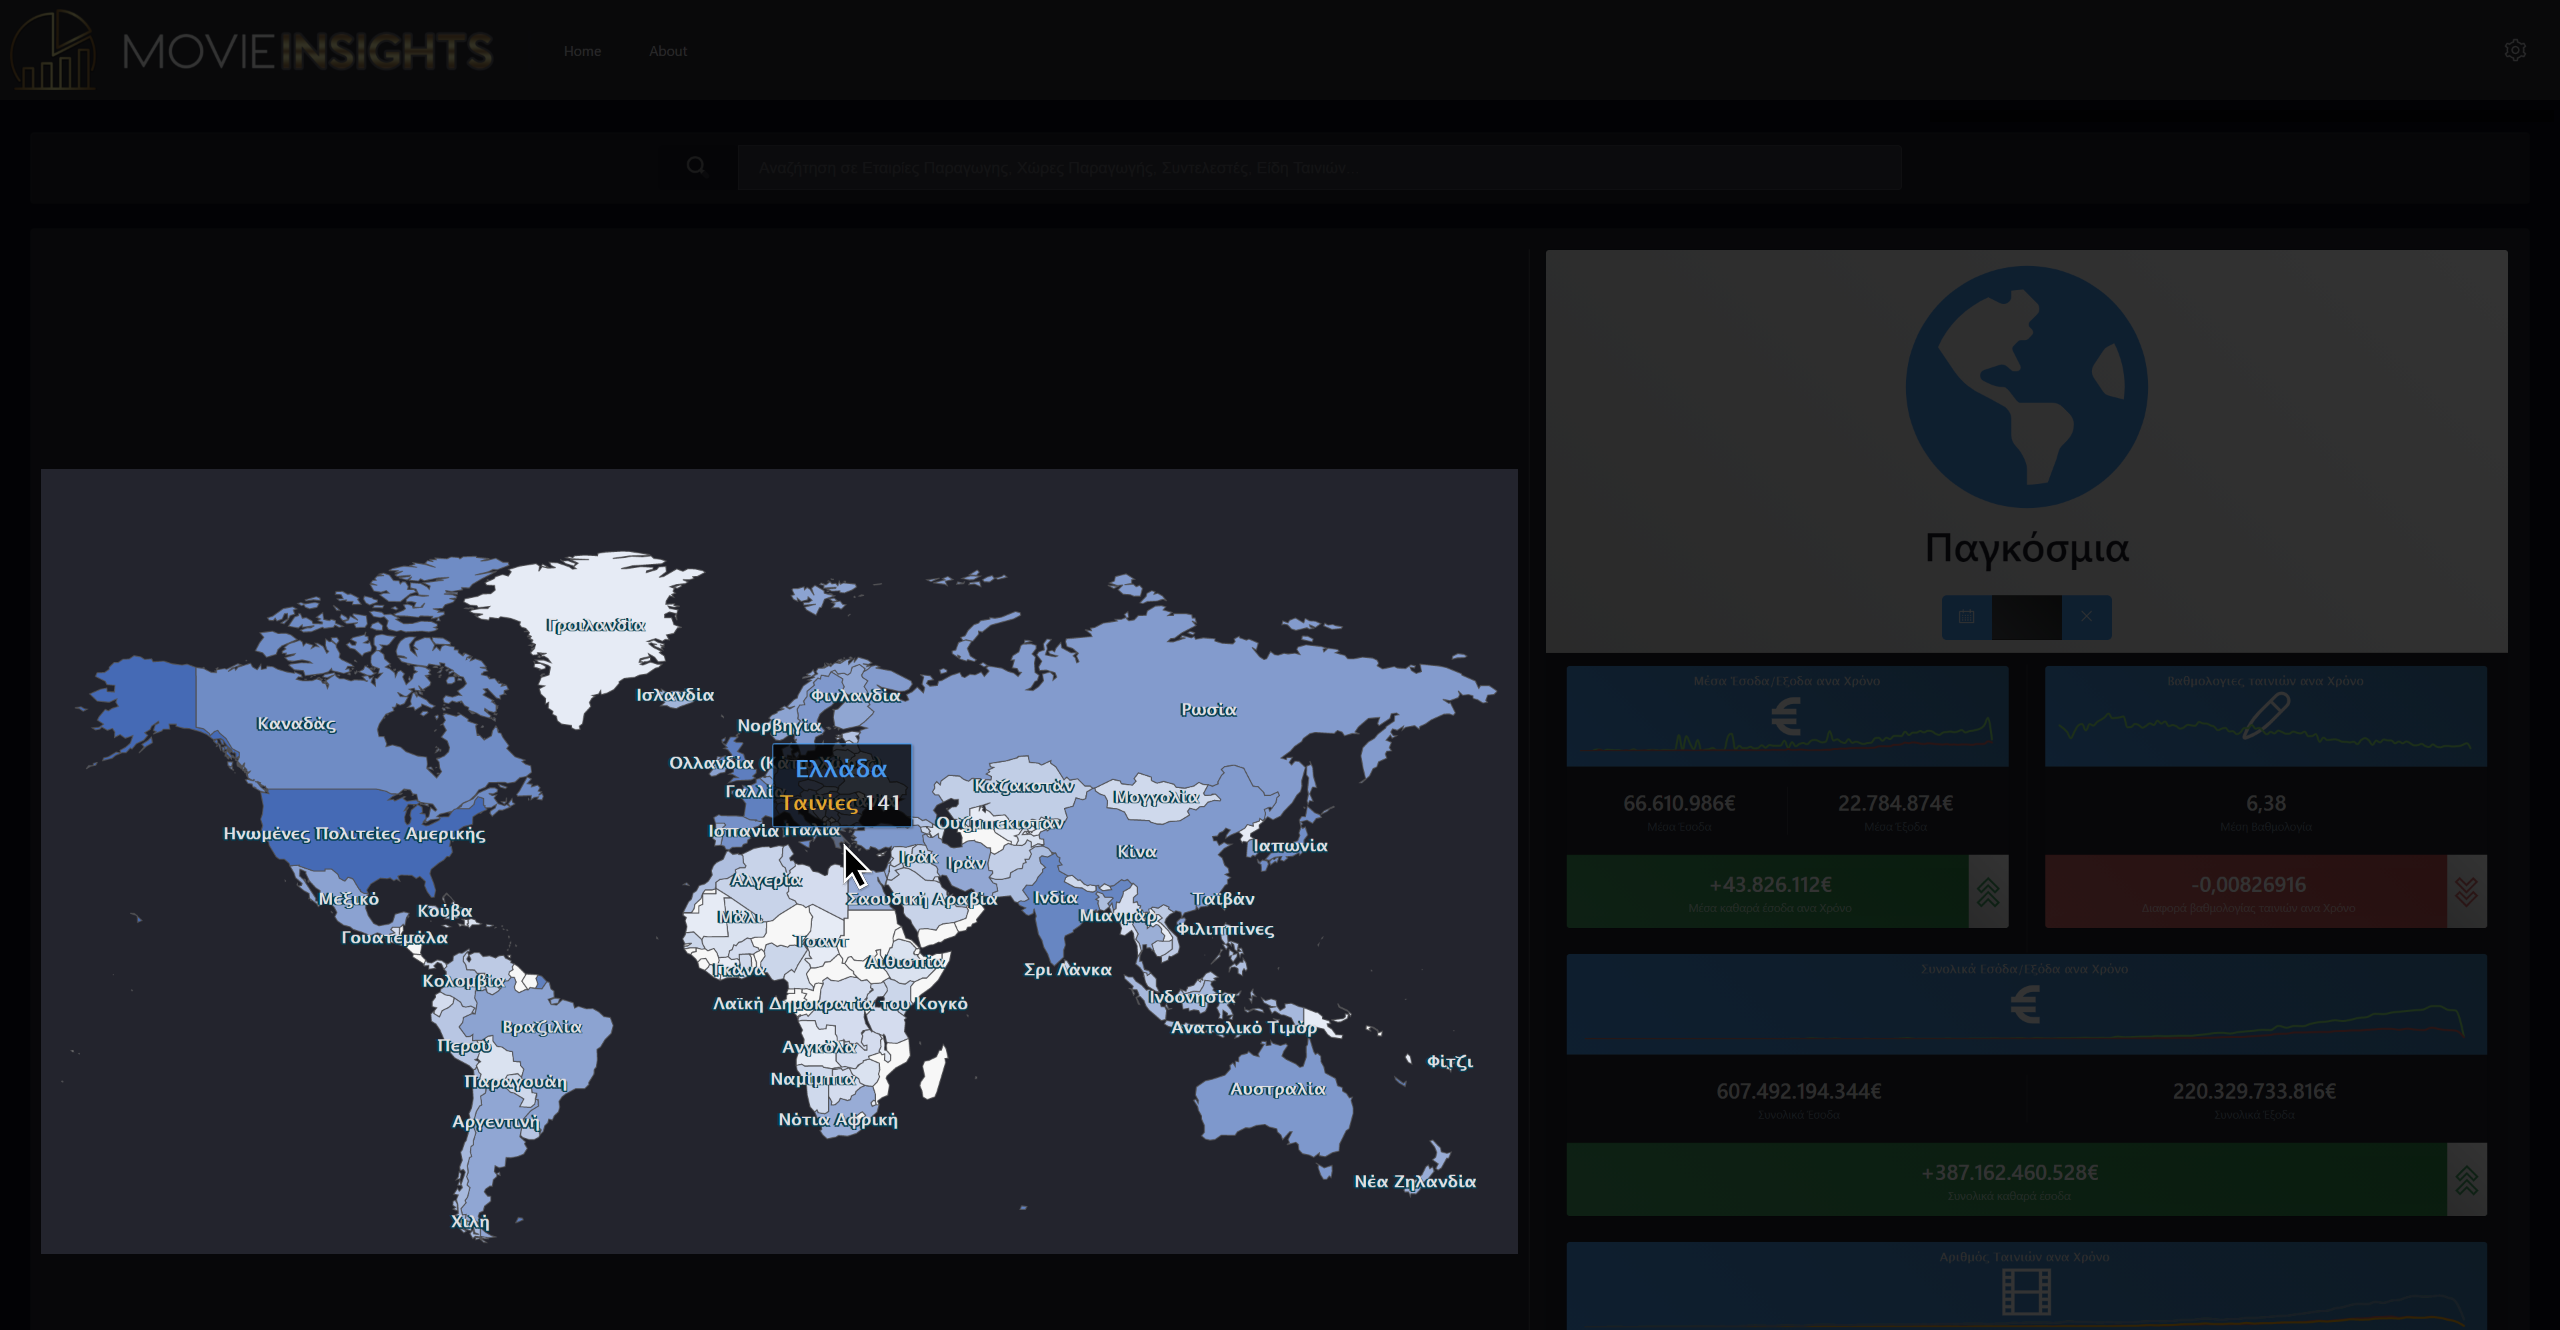
\includegraphics[width=145mm]{Chapters/6 - Manual/Images/main_page_map.png}
  \caption{Παγκόσμιος Χάρτης}
  \label{demo:map}
\end{figure}
\section{Πλαϊνή Στήλη}
Τώρα στην κατηγορία γενικών στοιχείων στα τα δεξιά του χάρτη βρίσκεται η στήλη με κάποια βασικά δεδομένα όπως φαίνεται στην εικόνα \ref{demo:sidebar}. Καθώς τα δεδομένα είναι πολλά πρέπει ο χρήστης να κυλίσει την σελίδα προς τα κάτω λίγο για να τα δει όλα. 

\begin{figure}[h]
  \centering
  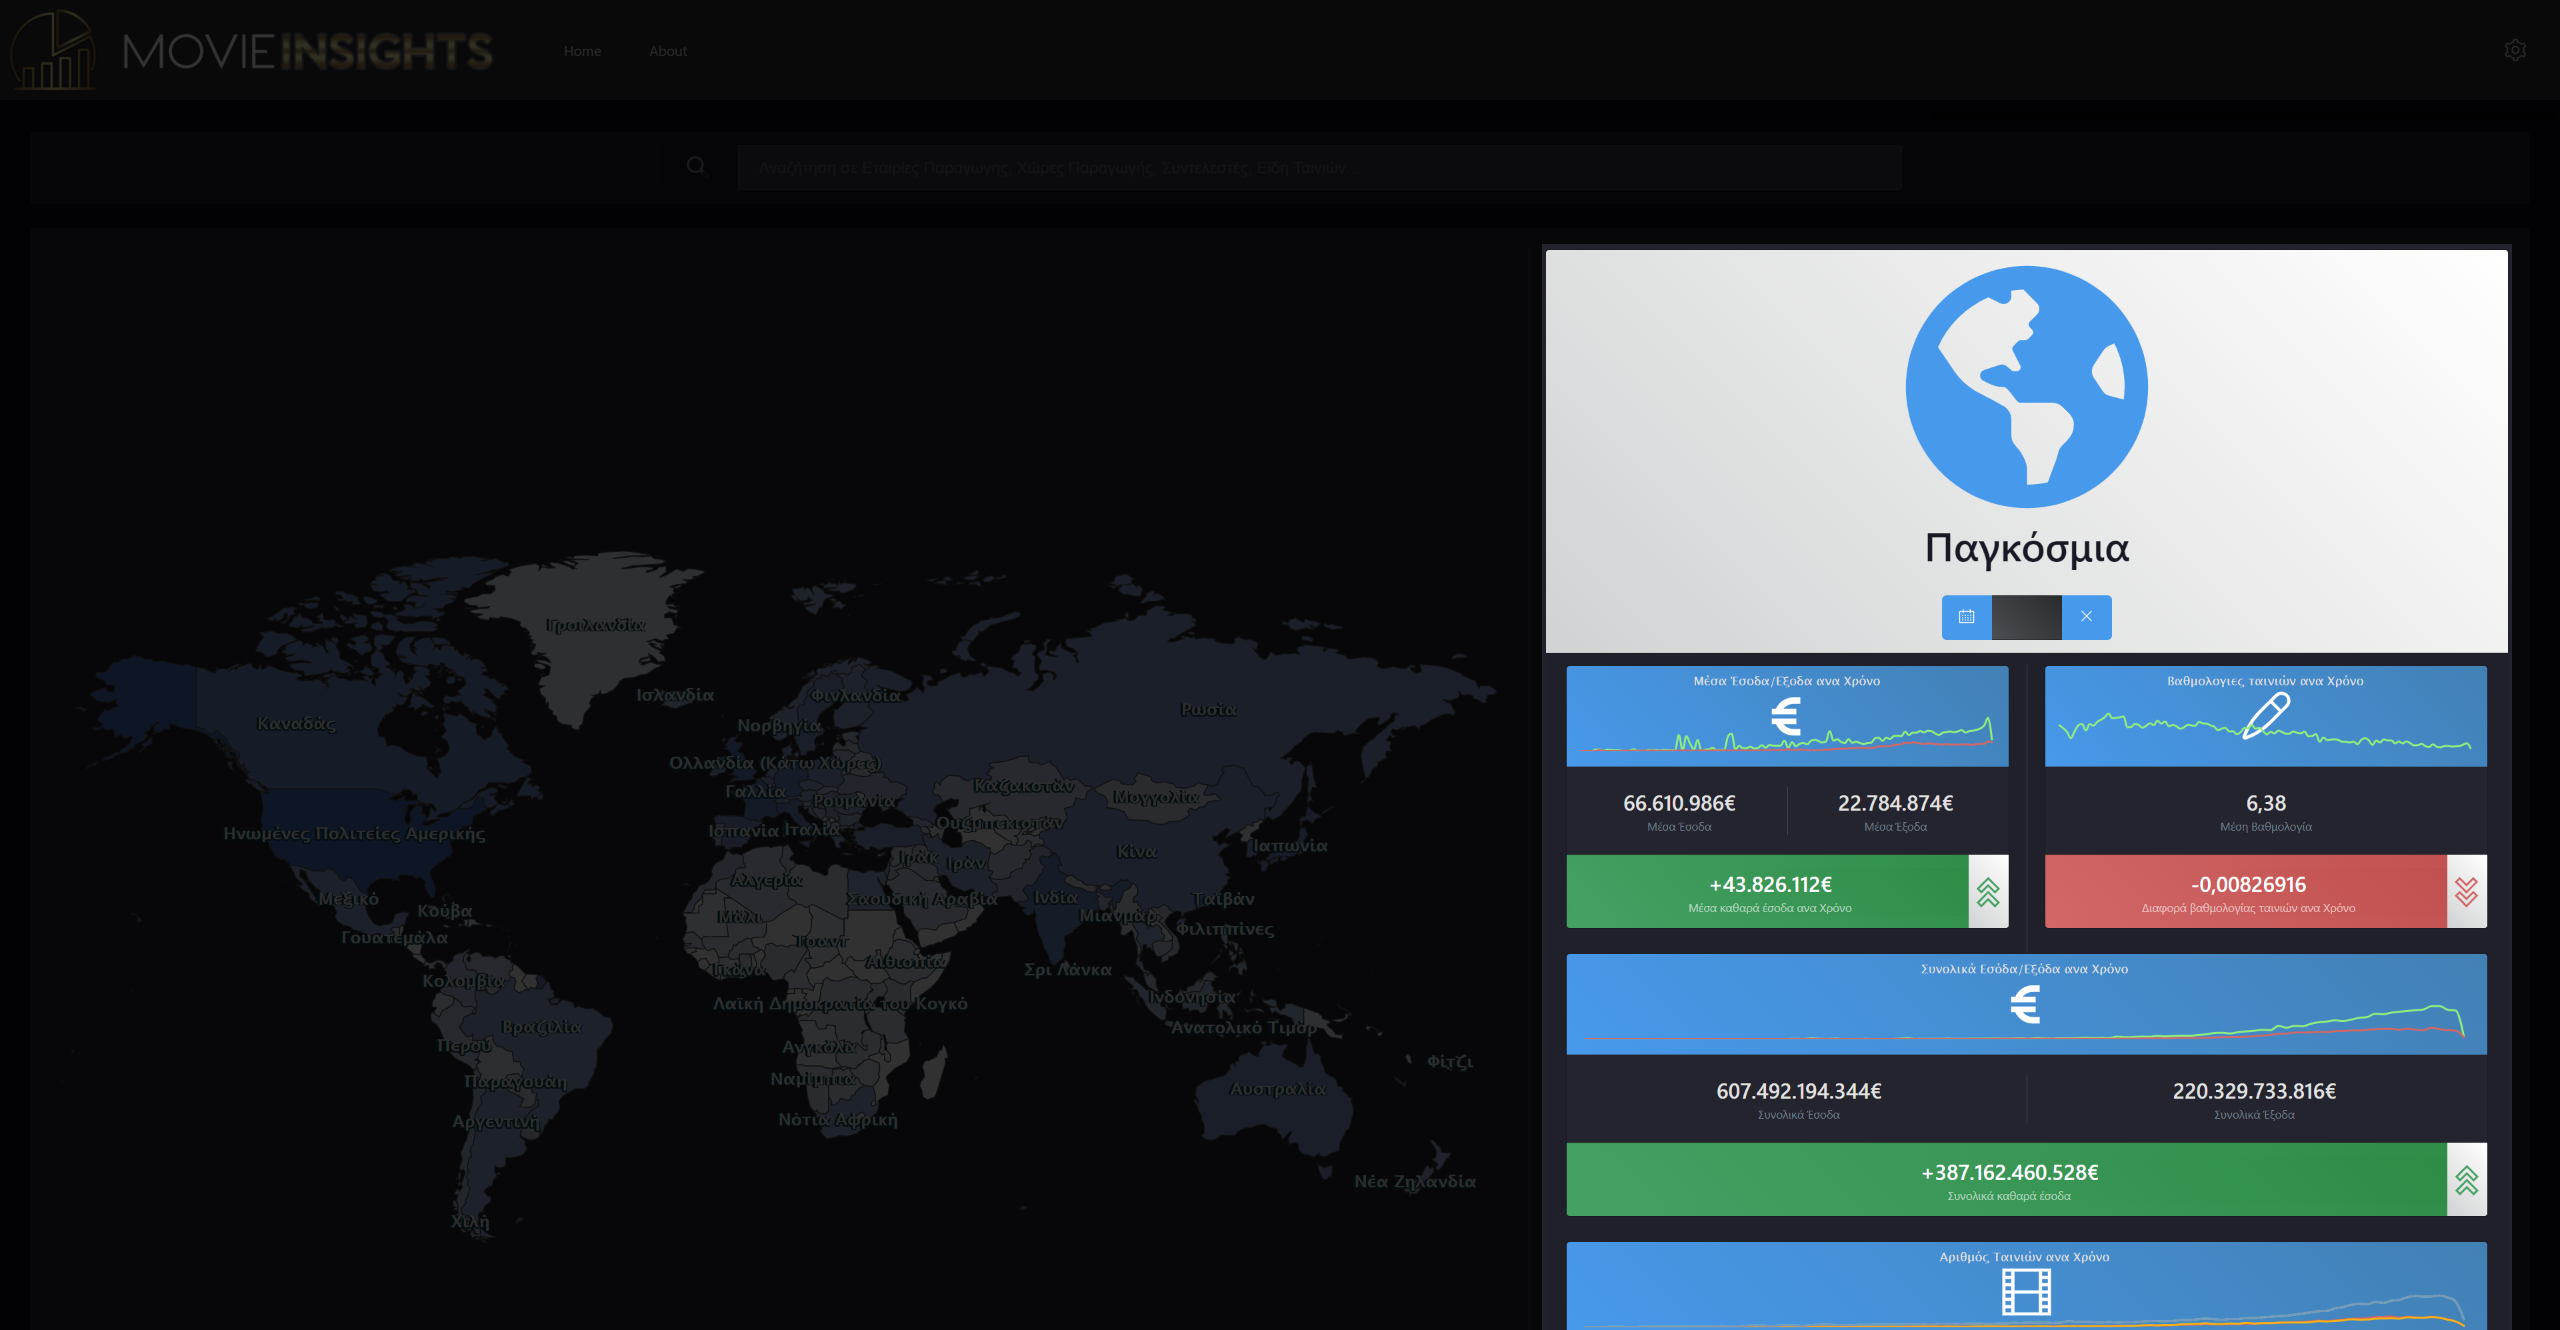
\includegraphics[width=145mm]{Chapters/6 - Manual/Images/main_page_sidebar.png}
  \caption{Πλαϊνή στήλη}
  \label{demo:sidebar}
\end{figure}

Στο πάνω το άσπρο μέρος της πλαϊνής στήλης, όπως φαίνεται στην εικόνα \ref{demo:sidebar_top}, βρίσκονται τα στοιχεία για το ποία κατηγορία βλέπουμε αυτήν την στιγμή που στην παρούσα κατάσταση είμαστε στην κατηγορία γενικών στοιχείων.
Περιέχει μια εικόνα που περιγράφει την κατηγορία που βρισκόμαστε στην προκειμένη περίπτωση καθώς είμαστε στα γενικά στοιχεία έχει επιλεγεί να εμφανιστεί μια υδρόγειος, περιέχει το όνομα της κατηγορίας που στην προκειμένη περίπτωση στην κατηγορία γενικών στοιχείων το όνομα είναι "Παγκόσμια" και περιέχει ένα πεδίο που επιτρέπει στον χρήστη να επιλέξει, είτε πατώντας στο εικονίδιο του ημερολογίου, είτε πατώντας στο πεδίο εισαγωγής, ένα έτος για να δει τα στοιχεία της κατηγορίας ανά έτος. Στα δεξιά του πεδίου εισαγωγής υπάρχει ένα εικονίδιο με το σύμβολο "X" που επιτρέπει τον χρήστη να καθαρίσει την επιλογή έτους για να δει ξανά τα συνολικά δεδομένα.

\begin{figure}[h]
  \centering
  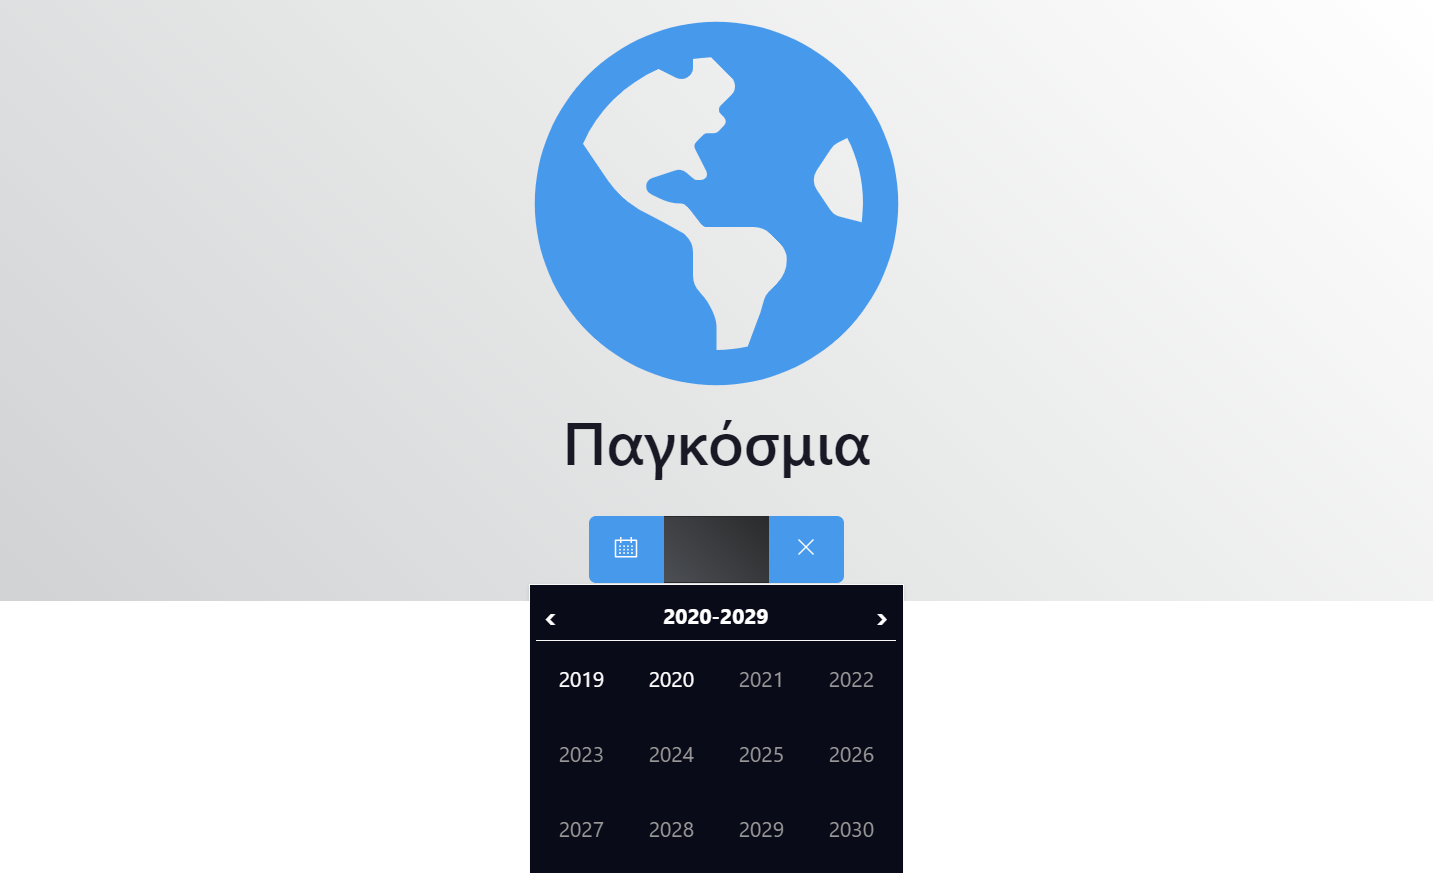
\includegraphics[width=75mm]{Chapters/6 - Manual/Images/main_page_sidebar_top.png}
  \caption{Πάνω μέρος πλαϊνής στήλης}
  \label{demo:sidebar_top}
\end{figure}

Στο πάνω μέρος της πλαϊνής στήλης όταν η κατηγορία είναι οποιαδήποτε άλλη πέρα των γενικών στοιχειών στο πάνω δεξιό μέρος εμφανίζεται ένα κουμπί με το σύμβολο "X", όπως φαίνεται στην εικόνα \ref{demo:sidebar_top_x}, το οποίο όταν πατηθεί επαναφέρει τον χρήστη στην κατηγορία γενικών στοιχείων. 

\begin{figure}[h]
  \centering
  
\includegraphics[width=110mm]{Chapters/6 - Manual/Images/main_page_sidebar_top_x.png}
  \caption{Κουμπί "Χ" στο πάνω μέρος πλαϊνής στήλης}
  \label{demo:sidebar_top_x}
\end{figure}

Το πάνω μέρος της πλαϊνής στήλης παραμένει το ίδιο για όλες τις κατηγορίες εκτός της κατηγορίας "ανά άτομο". Όταν η κατηγορία αναφέρεται σε ένα άτομο εμφανίζεται ένα ακόμα στοιχείο πάνω από το στοιχείο επιλογής έτους. Η εφαρμογή συλλέγει δεδομένα για ένα άτομο σε κατηγορίες. Συλλέγει δεδομένα για το άτομο σαν ηθοποιό, σαν παραγωγό, σαν σκηνοθέτη και σαν συγγραφέα. Για αυτό το λόγο σε εκείνο το σημείο υπάρχουν 4 κουμπιά που σου επιτρέπουν να επιλέξεις να δεις στοιχεία για ένα άτομο σε διαφορετικό ρόλο όπως φαίνεται στην εικόνα \ref{demo:sidebar_top_person}. Από προεπιλογή επιλέγεται ο ρόλος με τον οποίο εμφανίζεται πιο συχνά το άτομο αυτό. Δεν γίνεται να μην επιλεγεί κανένας ρόλος καθώς τα δεδομένα είναι διαφορετικά και βγαίνουν διαφορετικά συμπεράσματα για την πορεία του συγκεκριμένου ατόμου σε κάθε ρόλο. Όταν επιλεγεί ένας ρόλος το κουμπί που κρατάει αυτόν τον ρόλο θα γίνει μπλε. Όταν ένας ρόλος δεν είναι επιλεγμένος είναι σκούρο γκρι. Βέβαια ένα άτομο μπορεί να μην έχει γίνει για παράδειγμα ποτέ συγγραφέας ταινίας η σκηνοθέτης. Όταν λοιπόν δεν υπάρχουν δεδομένα για το συγκεκριμένο άτομο για έναν συγκεκριμένο ρόλο, το κουμπί που κατέχει αυτόν τον ρόλο θα απενεργοποιηθεί και θα χρωματιστεί με χρώμα ανοιχτό γκρι. Στην εικόνα βλέπουμε την ηθοποιό Margot Robbie, με προεπιλεγμένο ρόλο "ACTOR" για ηθοποιό και με έναν διαθέσιμο ακόμα ρόλο "PRODUCER", παραγωγό που σημαίνει ότι η εφαρμογή έχει στοιχεία για την Margot Robbie σαν ηθοποιό και σαν παραγωγό ταινιών αλλά δεν έχει δεδομένα σαν συγγραφέα η σκηνοθέτη. 

\begin{figure}[h]
  \centering
  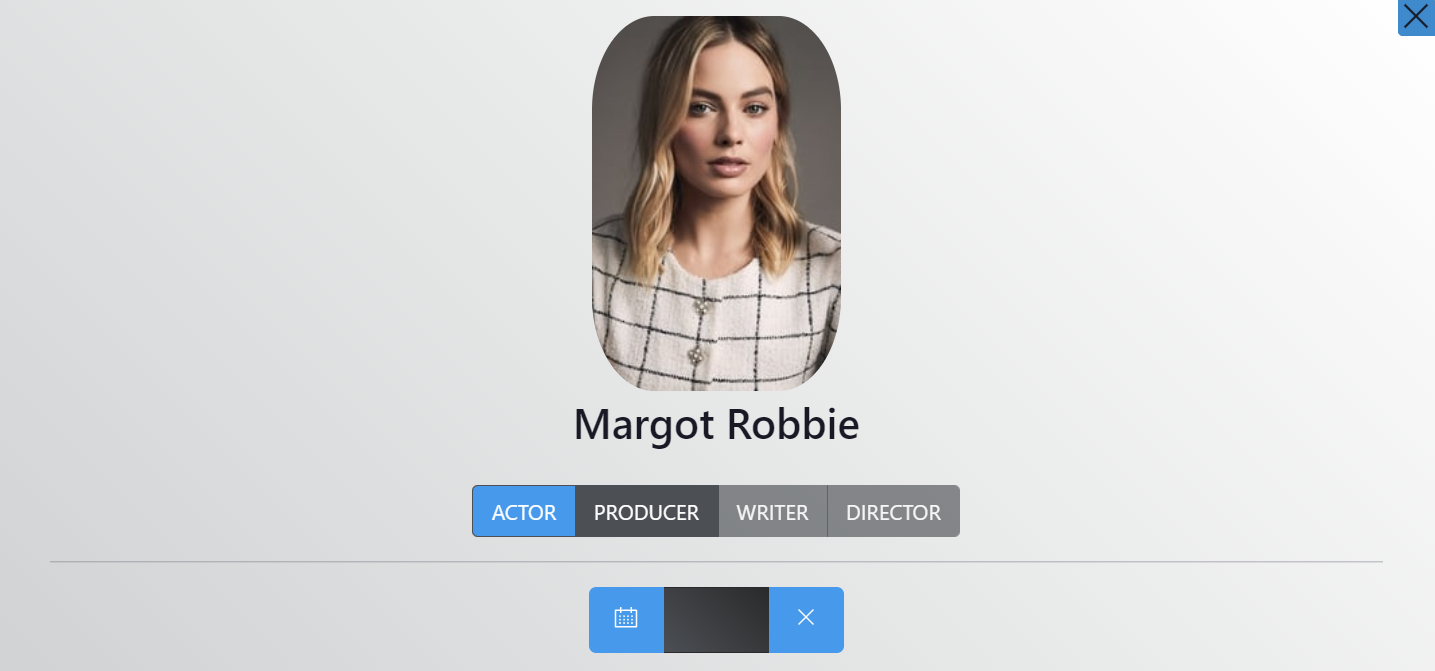
\includegraphics[width=110mm]{Chapters/6 - Manual/Images/main_page_sidebar_top_person.png}
  \caption{Επιλογή Ρόλου στο πάνω μέρος πλαϊνής στήλης}
  \label{demo:sidebar_top_person}
\end{figure}

Στο κάτω μέρος της πλαϊνής στήλης βρίσκονται 4 κάρτες δεδομένων όπως φαίνεται στην εικόνα \ref{demo:sidebar_bottom}.

\begin{figure}[h]
  \centering
  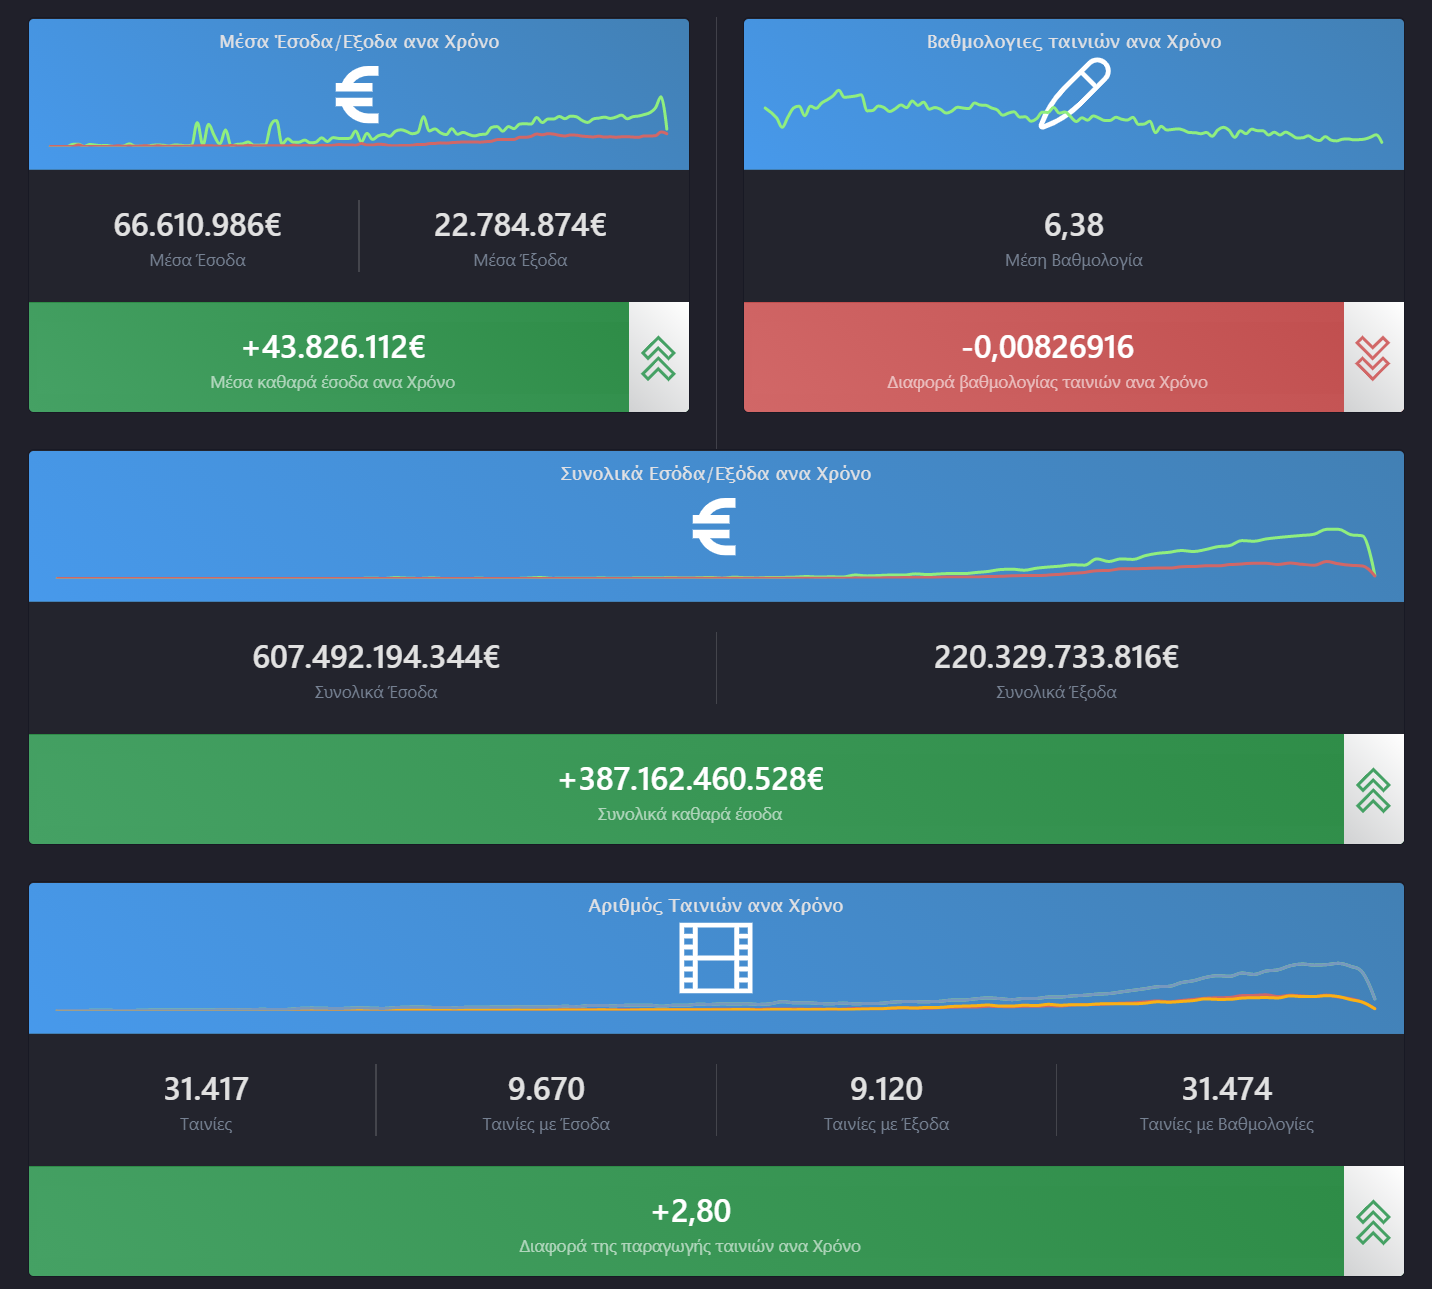
\includegraphics[width=75mm]{Chapters/6 - Manual/Images/main_page_sidebar_bottom.png}
  \caption{Πάνω μέρος πλαϊνής στήλης}
  \label{demo:sidebar_bottom}
\end{figure}

Η κάθε κάρτα περιέχει 3 κομμάτια και 4 καταστάσεις όπως φαίνεται στο σχήμα \ref{demo:sidebar_card}. Το πρώτο κομμάτι πάνω πάνω είναι ένα γράφημα το οποίο περιέχει ένα η περισσότερα ποσοτικά δεδομένα ανα χρόνο, τον τίτλο του γραφήματος για να γνωρίζει ο χρήστης τι κοιτάει καθώς και ένα περιγραφικό εικονίδιο για να γνωρίζει ο χρήστης τι είναι τα ποσοτικά δεδομένα που κοιτάει. Απο κάτω βρίσκεται το δεύτερο κομμάτι το οποίο περιέχει ενα η περισσότερα ποσοτικά δεδομένα που συνήθως είναι είτε τα μέγιστα, είτε τα ελάχιστα, είτε οι μέσοι όροι των δεδομένων των γραφημάτων. Το τρίτο και τελευταίο κομμάτι είναι ακριβώς απο κάτω και εμφανίζει συνήθως μια διαφορά τιμών ή έναν υπολογισμό δεδομένων με βάση τα προηγούμενα. 

\begin{figure}[h]
    \centering
    \begin{subfigure}[b]{0.475\textwidth}
        \centering
        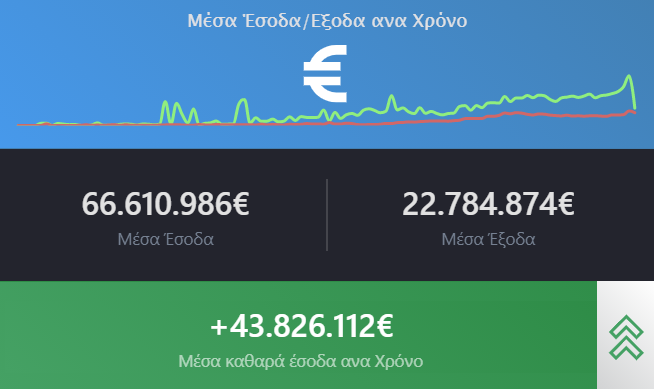
\includegraphics[width=\textwidth]{Chapters/6 - Manual/Images/main_page_sidebar_card_state1.png}
        \caption{Πρώτη κατάσταση}
        \label{demo:sidebar_card:state1}
    \end{subfigure}
    \hfill
    \begin{subfigure}[b]{0.475\textwidth}  
        \centering 
        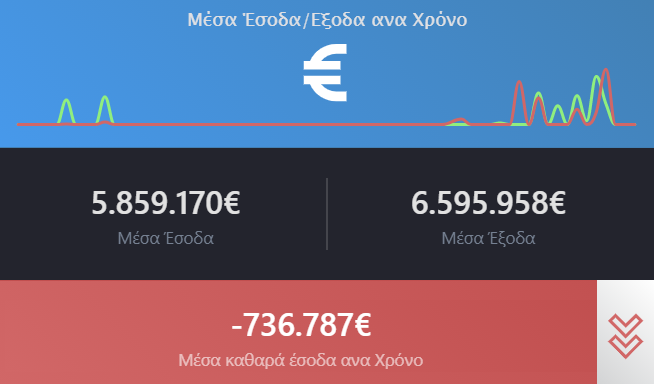
\includegraphics[width=\textwidth]{Chapters/6 - Manual/Images/main_page_sidebar_card_state2.png}
        \caption{Δεύτερη κατάσταση}
        \label{demo:sidebar_card:state2}
    \end{subfigure}
    \vskip\baselineskip
    \begin{subfigure}[b]{0.475\textwidth}   
        \centering 
        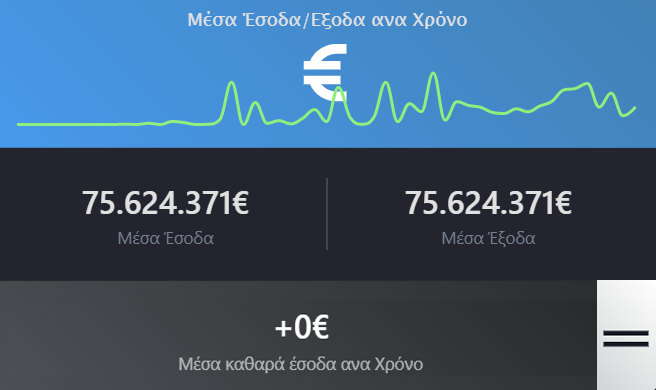
\includegraphics[width=\textwidth]{Chapters/6 - Manual/Images/main_page_sidebar_card_state3.png}
        \caption{Τρίτη κατάσταση}
        \label{demo:sidebar_card:state3}
    \end{subfigure}
    \hfill
    \begin{subfigure}[b]{0.475\textwidth}   
        \centering 
        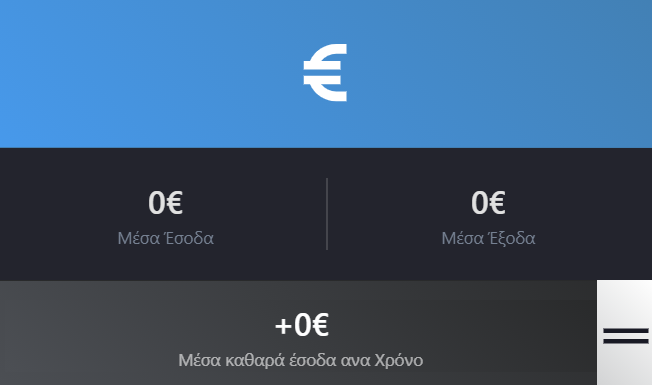
\includegraphics[width=\textwidth]{Chapters/6 - Manual/Images/main_page_sidebar_card_state4.png}
        \caption{Τέταρτη κατάσταση}
        \label{demo:sidebar_card:state4}
    \end{subfigure}
    \caption{Οι κάρτες της πλαϊνής στήλης και οι καταστάσεις τους}
    \label{demo:sidebar_card}
\end{figure}

Όπως προαναφέρθηκε μια κάρτα μπορεί να έχει 4 διαφορετικές καταστάσεις. Όταν η κατηγορία που βλέπει ο χρήστης έχει φιλτραριστεί ανά έτος τότε όλα τα γραφήματα όλων των καρτών, στο πρώτο κομμάτι, που αναφέρουν στοιχεία ανά χρόνο θα σβηστούν και ανάλογα με το τι δείχνει η κάρτα, τα άλλα 2 κομμάτια θα έχουν δεδομένα είτε θα μηδενιστούν όπως φαίνεται στην Κατάσταση 4 στο σχήμα \ref{demo:sidebar_card:state4}. Όταν δεν είναι φιλτραρισμένη η κατηγορία ανά έτος, αν το δεδομένο στο τρίτο κομμάτι της κάρτας είναι θετικό θα έχει χρώμα background πράσινο και στα δεξιά θα έχει ενα εικονίδιο με 2 βελάκια να δείχνουν προς τα πάνω όπως φαίνεται στο σχήμα της πρώτης κατάστασης \ref{demo:sidebar_card:state1}, αν είναι αρνητικό το χρώμα background θα είναι κόκκινο και στα δεξιά θα έχει ένα εικονίδιο με 2 βελάκια να δείχνουν προς τα κάτω όπως φαίνεται στο σχήμα της δεύτερης κατάστασης \ref{demo:sidebar_card:state2}, και αν είναι μηδέν τότε το χρώμα background θα είναι γκρι και το εικονίδιο στα δεξιά θα είναι 2 οριζόντιες γραμμές σαν το σύμβολο "ίσον" των μαθηματικών, όπως φαίνεται στο σχήμα της τρίτης κατάστασης \ref{demo:sidebar_card:state3}.

Η πρώτη κάρτα στην πλαϊνή στήλη εμφανίζει στο γράφημα τα μέσα έσοδα και τα έξοδα όλων των ταινιών στην συγκεκριμένη κατηγορία, και πιο συγκεκριμένα καθώς η κατηγορία η αρχική είναι τα συνολικά δεδομένα, εμφανίζει τα μέσα έσοδα / έξοδα όλων των ταινιών της βάσης δεδομένων. Αν ο χρήστης πάει τον κένσορα πάνω από το γράφημα εμφανίζεται ένα μικρό παράθυρο πάνω από τον κένσορα που αναγράφει το έτος και τα μέσα έσοδα έξοδα του έτους για την τοποθεσία που βρίσκεται ο κένσορας όπως φαίνεται στο σχήμα \ref{demo:sidebar_card:hover}. Απο κάτω αναφέρονται συνολικά κατά μέσο όρο τα μέσα έσοδα και έξοδα των ταινιών και στο τρίτο κομμάτι εμφανίζεται το μέσο καθαρό κέρδος των ταινιών συνολικά.

\begin{figure}[H]
  \centering
  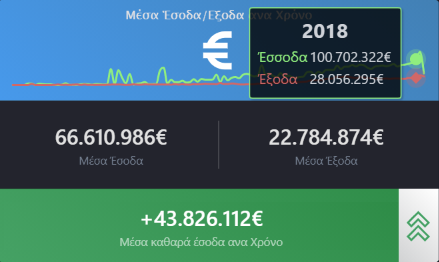
\includegraphics[width=75mm]{Chapters/6 - Manual/Images/main_page_sidebar_card_hover.png}
  \caption{Η Κάρτα με το παράθυρο απο πάνω}
  \label{demo:sidebar_card:hover}
\end{figure}

Στην δεύτερη κάρτα στο γράφημα εμφανίζονται οι μέσες βαθμολογίες των ταινιών ανά έτος. Στο δεύτερο κομμάτι εμφανίζεται συνολικά η μέση αξιολόγηση όλων των ταινιών της κατηγορίας και στο τρίτο κομμάτι εμφανίζεται η τάση των βαθμολογιών ανά χρόνο. Αυτό σημαίνει αν οι ταινίες μέσα στο πέρασμα των χρώνων έγιναν καλύτερες η χειρότερες. Αυτά τα δεδομένα φαίνονται στην εικόνα \ref{demo:sidebar_card:vote}.

\begin{figure}[H]
  \centering
  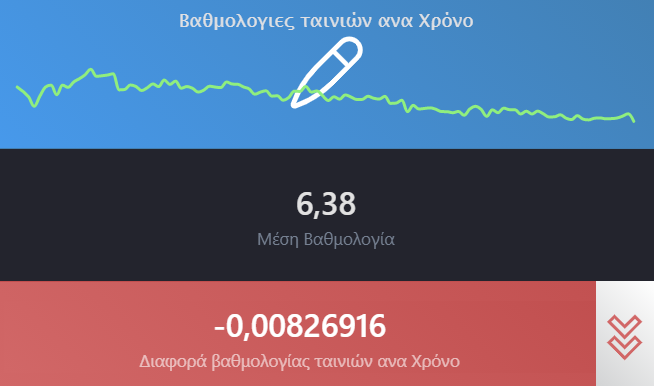
\includegraphics[width=75mm]{Chapters/6 - Manual/Images/main_page_sidebar_vote_card.png}
  \caption{Η Κάρτα βαθμολογιών}
  \label{demo:sidebar_card:vote}
\end{figure}

Η τρίτη κάρτα είναι ακριβώς το ίδιο με την πρώτη κάρτα με την διαφορά ότι αντί για τους μέσους εμφανίζει τα συνολικά δεδομένα, και η τέταρτη κάρτα αναγράφει κάποια στοιχεία για το νούμερο των ταινιών που υπάρχουν στην βάση δεδομένων και πόσες από αυτές παρέχουν δεδομένα εσόδων, εξόδων και βαθμολογιών.
\section{Κύρια Στοιχεία της Εφαρμογής}
Ακριβώς κάτω από τον χάρτη και την πλαϊνή στήλη βρίσκονται τα κύρια στοιχεία της εφαρμογής. Χωρίζονται σε 5 κατηγορίες "Ταινίες", "Συντελεστές", "Εταιρίες Παραγωγής", "Χώρες Παραγωγής" και "Ειδη Ταινιών" όπως φαίνεται στην εικόνα \ref{demo:insights}. 

\begin{figure}[H]
  \centering
  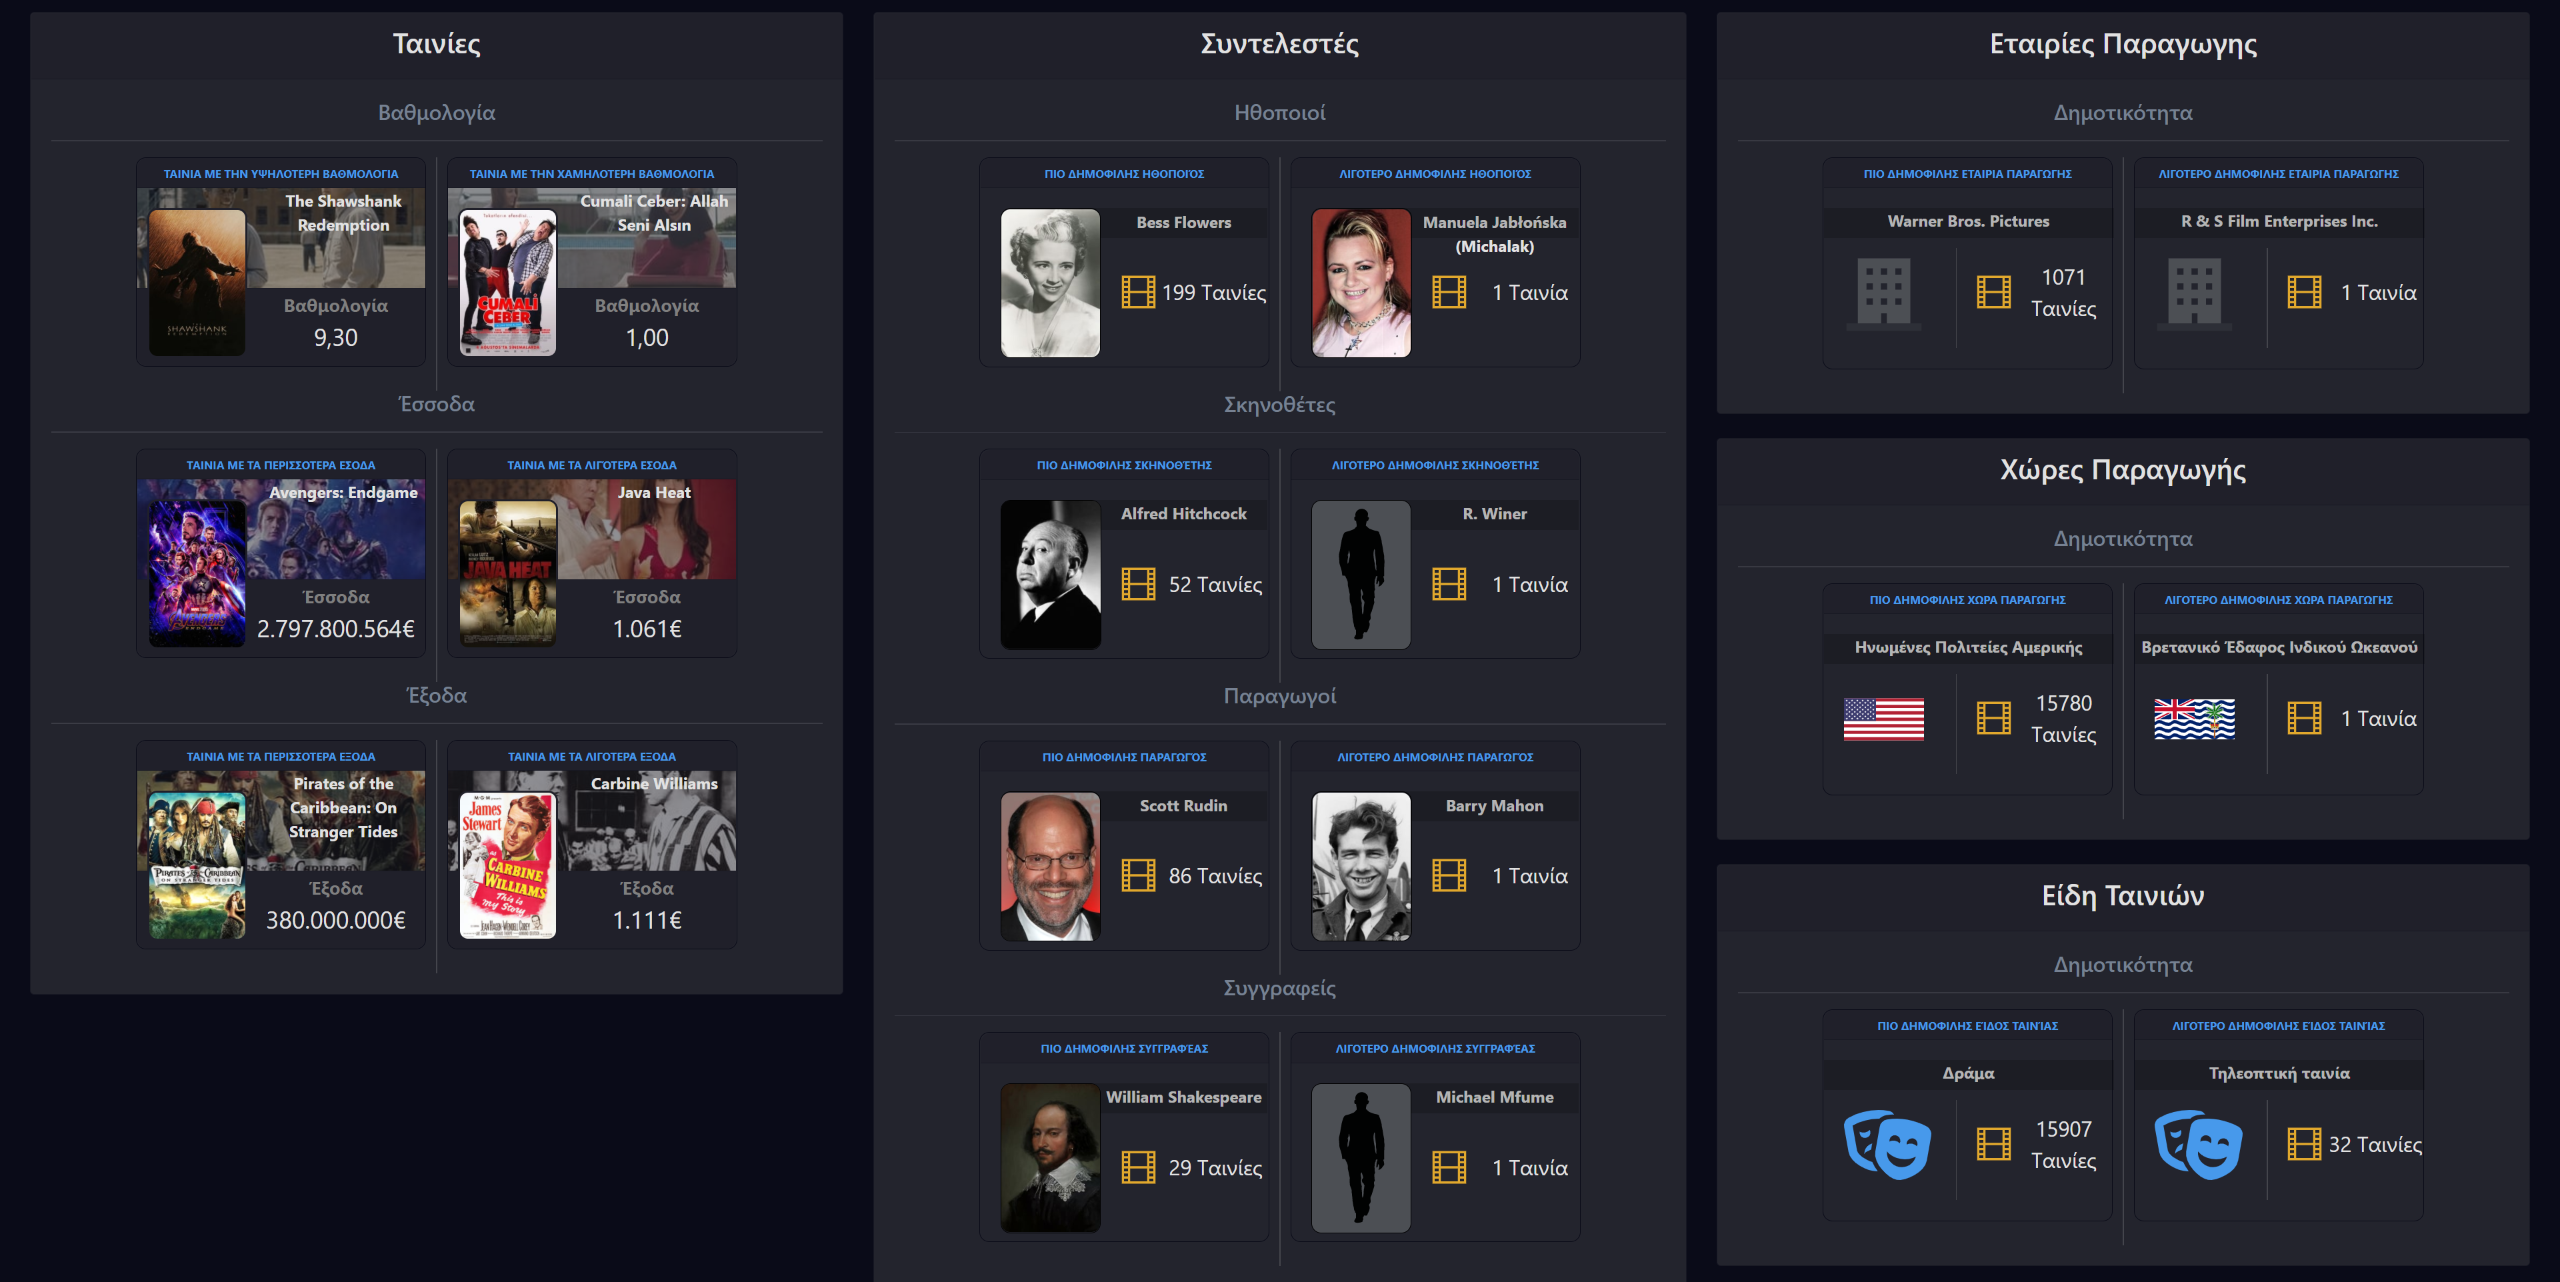
\includegraphics[width=145mm]{Chapters/6 - Manual/Images/main_page_insights.png}
  \caption{Κύρια Στοιχεία της εφαρμογής}
  \label{demo:insights}
\end{figure}

Στην κατηγορία των ταινιών προσφέρονται ταινίες με την μεγαλύτερη και μικρότερη βαθμολογία, και ταινίες με τα περισσότερα και λιγότερα έσοδα και έξοδα. Καθώς ο στόχος της εφαρμογής δεν είναι η προβολή αναλυτικών στοιχείων μιας ταινίας, όταν πατάει ο χρήστης πάνω σε μια από τις κάρτες που εμφανίζονται ανοίγει ένα παραθυράκι προσφέροντας κάποια πολύ βασικά δεδομένα όπως τα έσοδα, έξοδα, η βαθμολογία και ο χρόνος που διαρκεί αυτή η ταινία, και σε περίπτωση που ο χρήστης θέλει να δει παραπάνω στοιχεία για αυτήν την ταινία του επιτρέπεται από αυτό το παράθυρο να δει τα στοιχεία που θέλει είτε στην υπηρεσία Internet Movie DataBase (IMDB) είτε στην υπηρεσία The Movie Database (TMDb) όπως φαίνεται στην εικόνα \ref{demo:movie:modal}.

\begin{figure}[H]
  \centering
  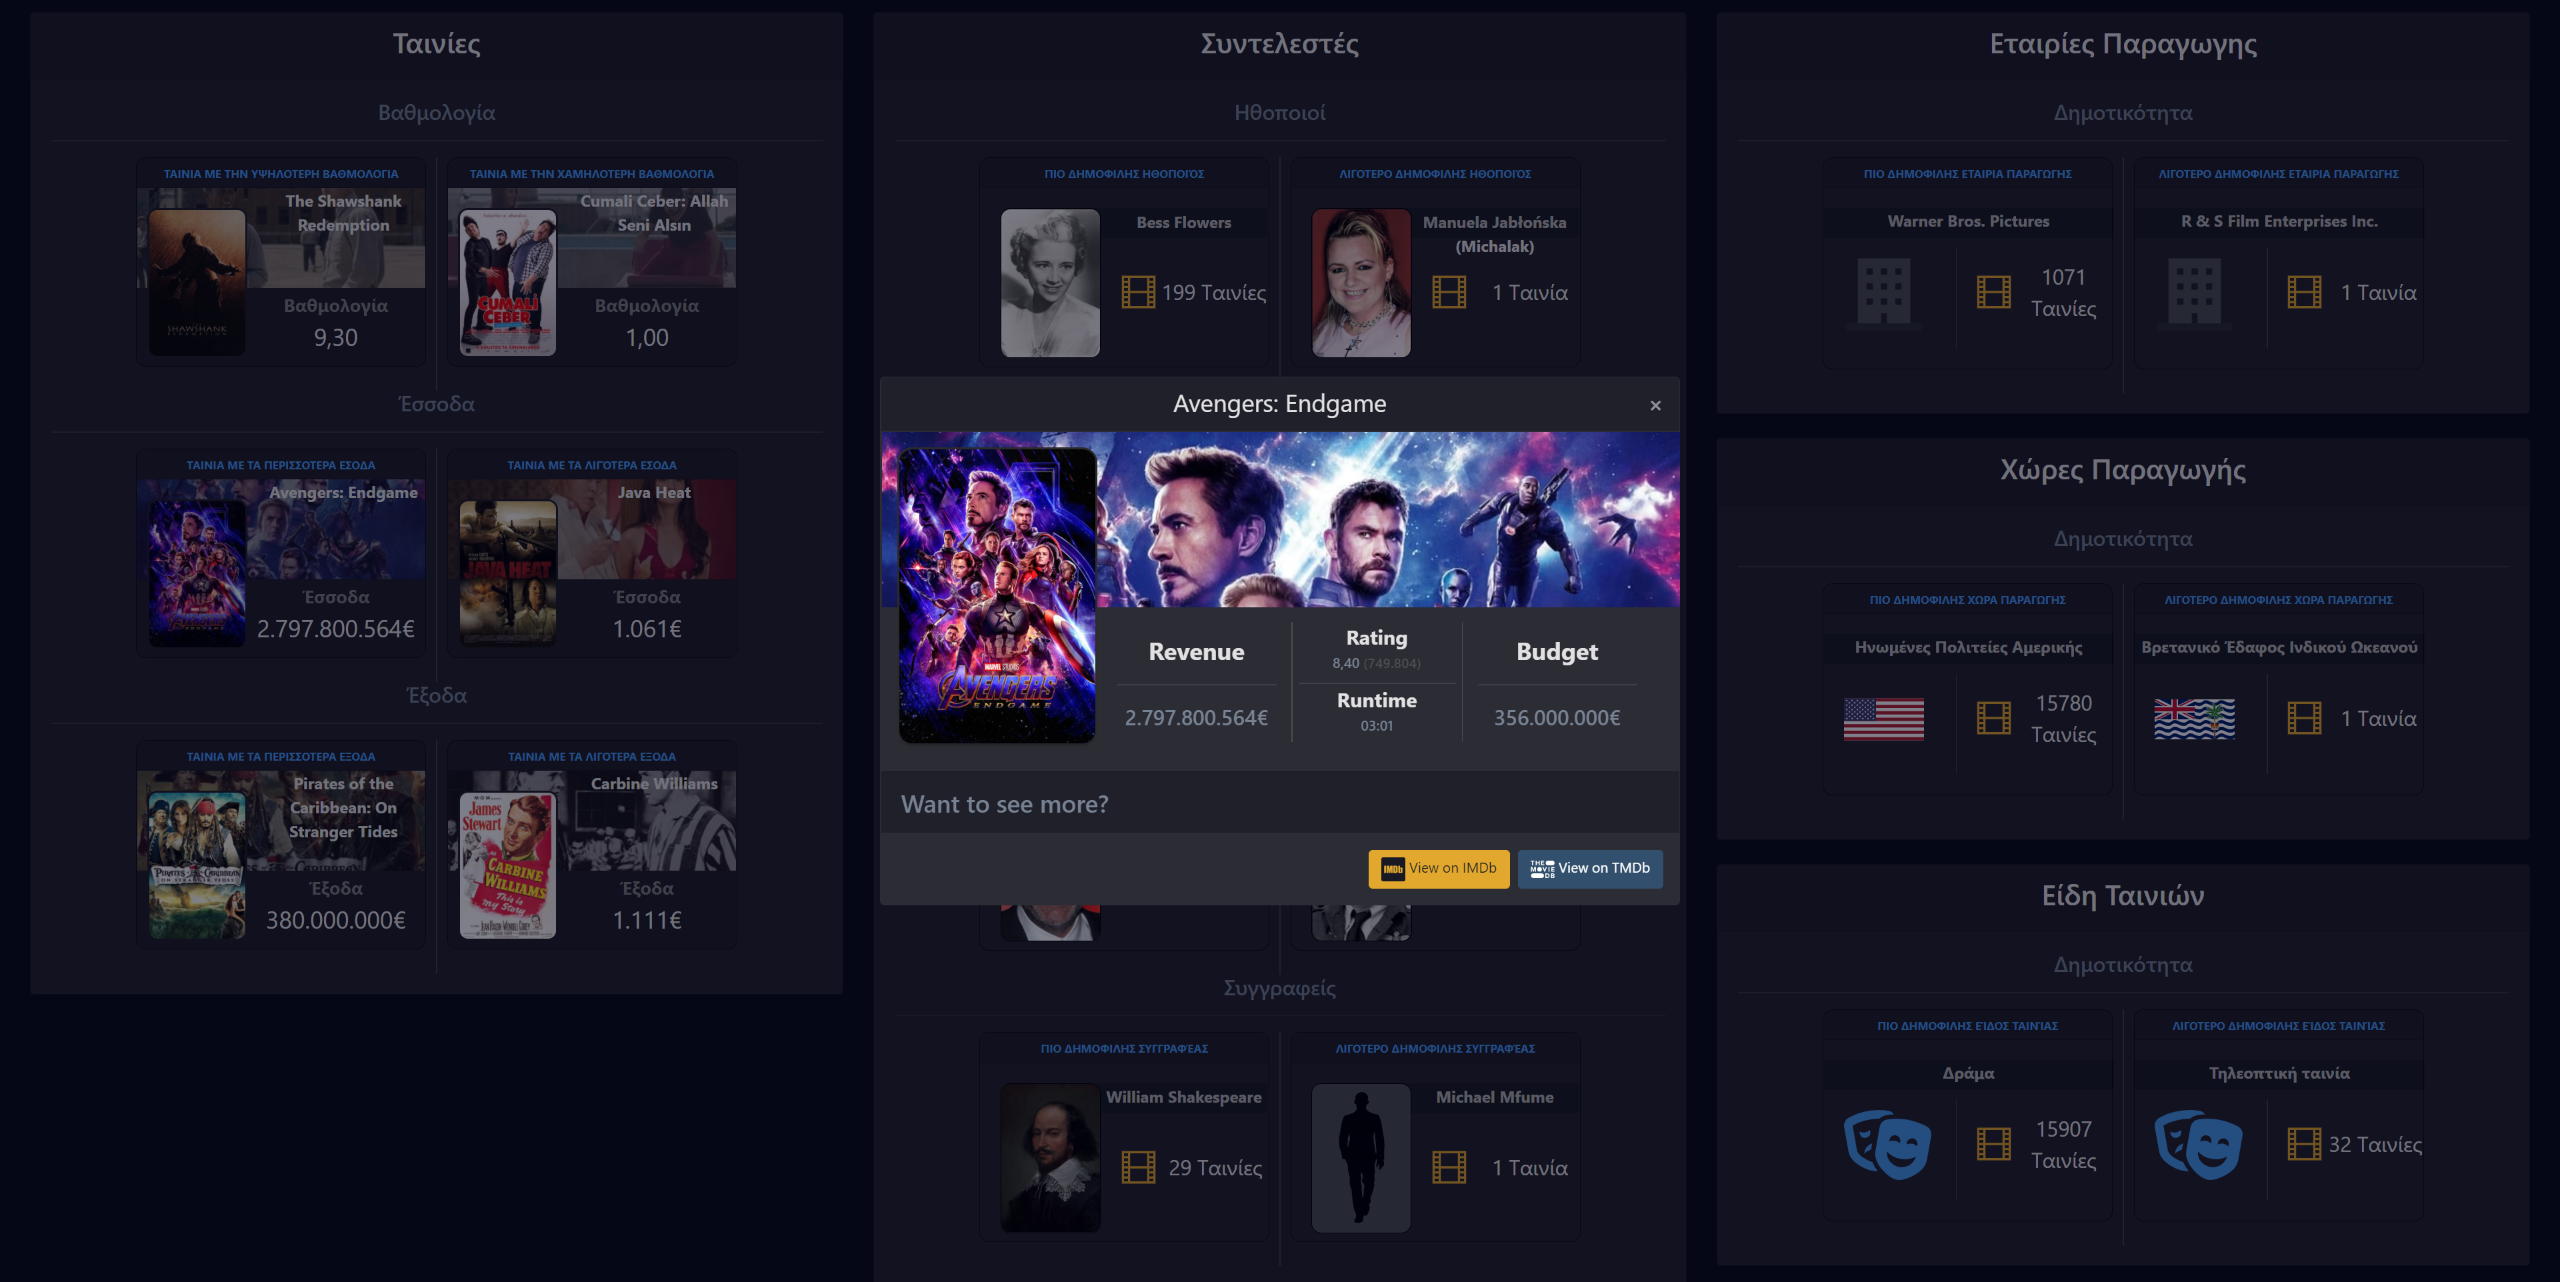
\includegraphics[width=145mm]{Chapters/6 - Manual/Images/main_page_insights_modal.png}
  \caption{Παράθυρο προβολής στοιχείων ταινίας}
  \label{demo:movie:modal}
\end{figure}

Στις υπόλοιπες κατηγορίες εμφανίζονται μόνο οι πιο δημοφιλής και λιγότερο δημοφιλής σε σχέση με την συμμετοχή τους σε ταινίες γενικότερα. Όταν ο χρήστης πατήσει σε μια κάρτα στις υπόλοιπες κατηγορίες η γενική κατηγορία της εφαρμογής θα αλλάξει και θα εμφανίσει στοιχεία της επιλογής του χρήστη.





\chapter{Συμπεράσματα}
Αν και η εφαρμογή αυτή είναι πλήρως λειτουργική κρύβει κάποια προβλήματα στην συνολική υλοποίηση της. Έχει έναν αρκετά γρήγορο τρόπο για τον υπολογισμό των δεδομένων που εξαρτάται σημαντικά από την επεξεργαστική ισχύ του μηχανήματος αλλά χρειάζεται να καταναλώσει ένα πάρα πολύ μεγάλο μέρος μνήμης RAM. Επίσης δεν υποστηρίζει ενημέρωση δεδομένων στην παρούσα κατάσταση της. Αν χρειαστεί να ενημερωθούν τα δεδομένα θα πρέπει να υπολογιστούν όλα από την αρχή, και όσα περισσότερα δεδομένα δοθούν για επεξεργασία τόση παραπάνω μνήμη θα καταναλώσει που φτάνει σε ένα σημείο θεωρητικά να μην γίνεται εφικτός ο υπολογισμός αυτών των δεδομένων αν ο όγκος των δεδομένων αυξηθεί σημαντικά.

Η παρούσα υλοποίηση δεν επιτρέπει επιπρόσθετα το Scaling. Αν αυτή η εφαρμογή γινόταν Viral δεν θα υπήρχε εφικτός τρόπος να γίνει Scale και να μπορέσει να εξυπηρετήσει όλους τους χρήστες που θα ζητούσαν δεδομένα.

Πάραυτα προσφέρει μία πληθώρα δεδομένων και ένα άτομο του χώρου της βιομηχανίας του κινηματογράφου μπορεί να τα βρει χρήσιμα για να μπορέσει να επιτελέσει το έργο του με μεγαλύτερη ευκολία.

\section{Στόχοι}
Οι στόχοι της πτυχιακής επιτεύχθηκαν στο σύνολό τους, 
με εξαίρεση κάποιων που επιλέχθηκε να μην υλοποιηθούν λόγω πρακτικών και τεχνικών προβλημάτων. Ένας από τους αρχικούς στόχους ήταν να υπολογιστούν με έναν συνδυασμό δεδομένων, συμπεράσματα για το πως μια ταινία έχει επηρεάσει τον τουρισμό στις χώρες και πόλεις γυρισμάτων. Καθώς θα ήταν ένα πολύ καλό μετρικό για την 
ανάδειξη της δύναμης των OpenData, η ίδια η απουσία των OpenData για αυτά τα δεδομένα, συνετέλεσε στην μη υλοποίησή αυτής της λειτουργίας. Ένας ακόμα αρχικός στόχος που δεν συμπεριλήφθηκε ήταν ένας Live χάρτης ο οποίος θα έδειχνε σε πραγματικό χρόνο για μία ταινία τις χώρες από τις οποίες κατεβάζεται πειρατικά. Αυτός ο στόχος δεν υλοποιήθηκε καθώς για την παρακολούθηση τέτοιων δεδομένων, έπρεπε η εφαρμογή να συμμετέχει σε μια τέτοια παράνομη ενέργεια και προτιμήθηκε η απόρριψη της. Για την περάτωση αυτής της λειτουργίας θα έπρεπε ο Server να υλοποιήσει το πρωτόκολλο Torrent, και να συμμετέχει στον παράνομο διαμοιρασμό των ταινιών έτσι ώστε να μπορεί να αναγνωρίσει μέσω των διευθύνσεων IP από ποιές χώρες κατεβάζονται πειρατικά οι ταινίες. Πολλοί Torrent Tracker καταπολεμούν την "παρακολούθηση" αρνούμενοι να δώσουν Peers σε Clients οι οποίοι δεν ζητάνε δεδομένα. Συνεπώς ο Client θα έπρεπε να κατεβάζει τα αρχεία αλλά και να αποθηκεύει τα δεδομένα καθώς οι Trackers ζητάνε και επαλήθευσή δεδομένων για να βεβαιωθούν ότι οι Clients τα κατεβάζουν. Πέρα από αυτό ο χειρισμός τέτοιων δεδομένων, όπως διευθύνσεις IP, ήθελαν εξαιρετικά ιδιαίτερο χειρισμό ειδικά με την νέα ευρωπαϊκή νομοθεσία GDPR.
Όλοι οι άλλοι στόχοι υλοποιήθηκαν με επιτυχία και υπάρχει ένα πολύ καλό αποτέλεσμα δείχνοντας ακριβώς γιατί είναι απαραίτητο πολλές εταιρίες να υιοθετήσουν το μοντέλο των OpenData. Όσα περισσότερα δεδομένα κυκλοφορούν ελεύθερα στο διαδίκτυο τόσες περισσότερες ιδέες και εργαλεία θα δημιουργούνται καθημερινά για την αξιοποίηση τους.

\section{Προτάσεις για εξέλιξη}
Όπως προαναφέρθηκε, η εφαρμογή αυτή είναι λειτουργική αλλά δεν είναι σε καμία περίπτωση έτοιμη για ένα Production περιβάλλον. Παρακάτω παρατίθενται κάποιες προτάσεις για την εξέλιξη του εν λόγω έργου και μελλοντικών βελτιστοποιήσεων. 

\begin{itemize}
    \item Καθώς η παρούσα υλοποίηση δεν υποστηρίζει Scaling, θα μπορούσε μελλοντικά να το υποστηρίξει χρησιμοποιώντας το μοντέλο των Microservices. 
    \item Θα μπορούσε να αλλάξει ριζικά ο αλγόριθμος υπολογισμού δεδομένων για να επιτρέπει την ενημέρωση των δεδομένων αντί για την συνολική επεξεργασία τους από την αρχή.
    \item Θα μπορούσε να δημιουργηθεί μια επιπρόσθετη λειτουργία στην υπηρεσία της εισαγωγής δεδομένων, έτσι ώστε να ελέγχει ανά τακτά χρονικά διαστήματα αν υπάρχουν νέα δεδομένα και να τα εισάγει αυτοματοποιημένα.
\end{itemize}

\section{Ο κώδικας}
Ο Κώδικας της εφαρμογής φιλοξενείται στο GitHub στην σελίδα: 

https://github.com/ProIcons/MovieInsights


%\citep{10.1007/978-3-540-76298-0_52}
%~\citep{Wikipedia_BibTeX}
% \chapter{Εισαγωγή5}
% \section{Η τυπογραφία σήμερα}
% Αυτή είναι η αναφορά σε ένα άρθρο περιοδικού:\citep{Schmidt98}.Αυτή
% είναι η αναφορά σε ένα βιβλίο:\citep{goosens93}. Αυτή είναι η αναφορά
% σε ένα ελληνικό βιβλίο:\citep{Chatzigeorgiou05}. Βιβλίο στα ελληνικά
% με ξένο συγγραφέα:\citep{Sommerville09}. Άρθρο σε
% συνέδριο~\citep{4343930}. 


% Τέλος αναφορά σε ιστοσελίδα:~\citep{Wikipedia_BibTeX}.

% Εδώ αναφερόμαστε στο σχήμα~\ref{fig:image1}:
% \begin{figure}[h]
%   \centering
%   
\includegraphics[width=35mm]{lion.png}
%   \caption{Παράδειγμα εικόνας}
%   \label{fig:image1}
% \end{figure}
% dsasdadadasdasdas
% ad
% asd
% asd

% και εδώ στον πίνακα~\ref{tab:table1}:
% \begin{table}[h]
%   \centering
%   \caption{Παράδειγμα πίνακα}
%  \begin{tabularx}{\linewidth}[h]{|XXX|}%
% \hline
% \hline
% Κίνητρα & Παραδείγματα ευρημάτων & Αριθμός μελετών\\
% \hline
% Ταύτιση με το έργο & Ξεκάθαροι στόχοι &20\\
% Καλό management & Ομαδικότητα &16\\
% Συμμετοχή υπαλλήλων & Συμμετοχή στις αποφάσεις&16\\
% Προοπτικές εξέλιξης & Προοπτικές προαγωγής&15\\
% Ποικιλία στην εργασία & Καλή χρήση ικανοτήτων& 14\\
% Αίσθηση του να ανήκεις κάπου& Υποστηρικτικές σχέσεις&14\\
% Αμοιβές και κίνητρα & Αυξημένος μισθός& 14\\
% \hline
% \hline
% \end{tabularx}
%   \label{tab:table1}
% \end{table}
% \appendix
% \chapter{Συνοπτικός οδηγός χρήσης \LaTeX}
% Εδώ βάζετε ότι θα έμπαινε σε παράρτημα.
% \texttt{Δοκιμή σε mono-space}
%Προαιρετικά

\begin{Glossary}
\begin{description}
\item[TCP]Transmission Control Protocol
\item[DSL]Domain Specific Language
\item[JSON]JavaScript Object Notation
\item[XML]eXtensible Markup Language
\item[IoC]Inversion of Control
\item[Java EE]Java Enterprisse Edition
\item[SPA]Single Page Application
\item[API]Application Programming Interface
\item[IoC]Inversion of Control
\item[TSV]Tab-Separated Values
\item[JVM]Java Virtual Machine
\item[CRUD]\textbf{C}reate, \textbf{R}ead, \textbf{U}pdate and \textbf{D}elete
\end{description}
\end{Glossary}
\printbibliography[heading=bibintoc,title={Βιβλιογραφία}]
\lastpageinfo
\end{document}
